\documentclass[msc,lith,english]{liuthesis}
%% Settings go in settings.tex
\input{settings}
\usepackage{rotating}
\usepackage{color}
\usepackage{url}

% \usepackage{changebar}

\usepackage{comment}

%%%%%%%%%%%%%%%%% GRAPHVIZ %%%%%%%%%%%%%%%%%%%
\usepackage[pdf]{graphviz}
\usepackage{float}    % For the [H] placement specifier
\usepackage{dot2texi}

%%%%%%%%%%%%%%%%% GANTT CHART %%%%%%%%%%%%%%%%%%%
\usepackage{pgfgantt}
\usepackage{tikz}
\usepackage{pgfgantt}
\usepackage{graphicx} % Required for rotation
%Used to draw gantt charts, which I will use for the calendar.
%Let's define some awesome new ganttchart elements:
\newganttchartelement{orangebar}{
    orangebar/.style={
        inner sep=0pt,
        draw=red!66!black,
        very thick,
        top color=white,
        bottom color=orange!80
    },
    orangebar label font=\slshape,
    orangebar left shift=.1,
    orangebar right shift=-.1
}

\newganttchartelement{bluebar}{
    bluebar/.style={
        inner sep=0pt,
        draw=purple!44!black,
        very thick,
        top color=white,
        bottom color=blue!80
    },
    bluebar label font=\slshape,
    bluebar left shift=.1,
    bluebar right shift=-.1
}

\newganttchartelement{greenbar}{
    greenbar/.style={
        inner sep=0pt,
        draw=green!50!black,
        very thick,
        top color=white,
        bottom color=green!80
    },
    greenbar label font=\slshape,
    greenbar left shift=.1,
    greenbar right shift=-.1
}


%%%%%%%%%%%%%%%% CODE BLOCKS %%%%%%%%%%%%%%%%%%%%%%%%%
\usepackage{listings}
\usepackage{xcolor}
\definecolor{codegreen}{rgb}{0,0.6,0}
\definecolor{codegray}{rgb}{0.5,0.5,0.5}
\definecolor{codepurple}{rgb}{0.58,0,0.82}
\definecolor{backcolour}{rgb}{0.95,0.95,0.92}

    
\lstdefinestyle{python}{
    backgroundcolor=\color{backcolour},   
    commentstyle=\color{codegreen},
    keywordstyle=\color{magenta},
    numberstyle=\scriptsize,
    stringstyle=\color{codepurple},
    basicstyle=\normalfont\ttfamily,
    breakatwhitespace=false,         
    breaklines=true,                 
    captionpos=b,                    
    keepspaces=true,                 
    numbers=left,                    
    numbersep=8pt,                  
    showspaces=false,                
    showstringspaces=false,
    showtabs=false,
    frame=single,   % or lines
    tabsize=2
}
\lstset{style=python}

\colorlet{punct}{red!60!black}
\colorlet{delim}{brown!80!black}


\lstdefinelanguage{json}{
    basicstyle=\normalfont\ttfamily,
    numbers=left,
    numberstyle=\scriptsize,
    stepnumber=1,
    numbersep=8pt,
    showstringspaces=false,
    frame=single,   % or lines
    breaklines=false,        % Enables line breaking
    breakatwhitespace=false,
    backgroundcolor=\color{backcolour},
    literate=
      {:}{{{\color{punct}{:}}}}{1}
      {,}{{{\color{punct}{,}}}}{1}
      {\{}{{{\color{delim}{\{}}}}{1}
      {\}}{{{\color{delim}{\}}}}}{1}
      {[}{{{\color{delim}{[}}}}{1}
      {]}{{{\color{delim}{]}}}}{1},
}


\lstdefinelanguage{bash}{
    basicstyle=\normalfont\ttfamily,
    numbers=left,
    numberstyle=\scriptsize,
    stepnumber=1,
    numbersep=8pt,
    showstringspaces=false,
    frame=single,   % or lines
    breaklines=false,        % Enables line breaking
    breakatwhitespace=false,
    backgroundcolor=\color{backcolour},
    literate=
      {:}{{{\color{punct}{:}}}}{1}
      {,}{{{\color{punct}{,}}}}{1}
      {\{}{{{\color{delim}{\{}}}}{1}
      {\}}{{{\color{delim}{\}}}}}{1}
      {[}{{{\color{delim}{[}}}}{1}
      {]}{{{\color{delim}{]}}}}{1}
      {├}{|-}2 {└}{`-}2 {─}{-}1 {│}{|}1,
}


\usepackage[edges]{forest}

\definecolor{foldercolor}{RGB}{124,166,198}

\tikzset{pics/folder/.style={code={%
    \node[inner sep=0pt, minimum size=#1](-foldericon){};
    \node[folder style, inner sep=0pt, minimum width=0.3*#1, minimum height=0.6*#1, above right, xshift=0.05*#1] at (-foldericon.west){};
    \node[folder style, inner sep=0pt, minimum size=#1] at (-foldericon.center){};}
    },
    pics/folder/.default={20pt},
    folder style/.style={draw=foldercolor!80!black,top color=foldercolor!40,bottom color=foldercolor}
}

\forestset{is file/.style={edge path'/.expanded={%
        ([xshift=\forestregister{folder indent}]!u.parent anchor) |- (.child anchor)},
        inner sep=1pt},
    this folder size/.style={edge path'/.expanded={%
        ([xshift=\forestregister{folder indent}]!u.parent anchor) |- (.child anchor) pic[solid]{folder=#1}}, inner xsep=0.7*#1},
    folder tree indent/.style={before computing xy={l=#1}},
    folder icons/.style={folder, this folder size=#1, folder tree indent=3*#1},
    folder icons/.default={12pt},
}


%%%%%%%%%%%% COOL LOOKING PIECHART FOR RESULT CATEGORIZATION DISTRIBUTION %%%%%%%%%%%%%%
\usepackage[svgnames]{xcolor}
\usepackage{tikz,ifthen}

% "The fourier package replaces LaTeX’s default Computer Modern (CM) fonts with the “Fourier‑Utopia” text and math family. As soon as TeX reads that package, every piece of type in your document—headings, body text, equations—switches to Utopia, so it looks as though “something” in the diagram code changed the font."
\usepackage{fourier}

\usetikzlibrary{calc}

\newcommand{\degre}{$^\circ$}

% ——— Other colors ————————————
\definecolor{correct_color}{HTML}{7DCE82}
\definecolor{incorrect_color}{HTML}{FF5E5B}
\colorlet{correct_color}{correct_color}
\colorlet{incorrect_color}{incorrect_color}

\definecolor{weak_correct_color}{HTML}{F2FAF2}
\colorlet{weak_correct_color}{weak_correct_color}

\definecolor{weak_incorrect_color}{HTML}{FFEEEE}
\colorlet{weak_incorrect_color}{weak_incorrect_color}

\definecolor{default_bar_color}{HTML}{2AB6CB}
\colorlet{default_bar_color}{default_bar_color}

% ——— Graph overview ————————————
\definecolor{unique1}{HTML}{FA9638}   % critical
\definecolor{unique2}{HTML}{73A1AB}   % non-critical
\definecolor{unique3}{HTML}{C5C5C5}   % uncategorized

% ——— Graph critical ———————
\definecolor{crit1}{HTML}{FEF4EB}
\definecolor{crit2}{HTML}{FDDEC4}
\definecolor{crit3}{HTML}{FBB574}
\definecolor{crit4}{HTML}{FCC574}
\definecolor{crit5}{HTML}{F78B26}
\definecolor{crit6}{HTML}{D96D08}

% ——— Graph non-critical ———————
\definecolor{noncrit1}{HTML}{CCDDE0}
\definecolor{noncrit2}{HTML}{A6C4C9}
\definecolor{noncrit3}{HTML}{81AAB1}
\definecolor{noncrit4}{HTML}{5D8F98}

%%%% Critical cats
\colorlet{color0}{crit1}
\colorlet{color1}{crit2}
\colorlet{color2}{crit3}
\colorlet{color3}{crit4}
\colorlet{color4}{crit5}
\colorlet{color5}{crit6}

%%%% Non-Critical cats
\colorlet{color6}{noncrit1}
\colorlet{color7}{noncrit2}
\colorlet{color8}{noncrit3}
\colorlet{color9}{noncrit4}

%%%% Unique changes distr
\colorlet{color10}{unique1}
\colorlet{color11}{unique2}
\colorlet{color12}{unique3}


\makeatletter
    \tikzset{%
        dc tag/.style={align=center},
        dc legend/.style={align=left,anchor=west},
        dc sector/.style={fill=\Cj,line join=round}
        }

    \pgfkeys{/DiagCirc/.cd,
        % liste of \Name/Value
        value list/.store in=\Value@list,
        % circular : 360 - semi circular 180
        angle max/.store in=\Angle@max,
        angle max=360,
        % radius of the diagram
        radius/.store in=\R@dius,
        radius=4cm,
        % composition of the legend
        % \V value
        % \N name
        % \P percent
        % \A angle
        % \Cj color
        legend/.store in=\L@gend,
        legend=,
        % location of the legend
        legend location/.store in=\Legend@Loc,
        legend location={($(\R@dius,\R@dius)+(.5,-.5)$)},   
        % poisition of the node in the sector
        % 0 center, 1 on the edge, 1.++ external
        factor/.store in=\F@ctor,
        factor=.80,
        % composition of the node in the sector
        tags/.store in=\T@gs,
        tags=,
        % correction of round errors in percents
        percent corr/.store in=\C@rrP,
        percent corr=,
        % correction of round errors in angles
        angle corr/.store in=\C@rrA,
        angle corr=,
        % individual shift
        shift sector/.store in=\Shift@j,
        shift sector=,
        % more nodes in the sectors, or new legeng
        sup loop/.store in=\Sup@Loop,
        sup loop=,
        % ----- *** NEW *** explicit colour list -----------------------------------
        color list/.store in=\Color@list,
        color list=,
        % ----- main drawing macro --------------------------------------------------
        diagram/.code={%
        % Calculation of the sum
        \pgfmathsetmacro\S@m{0}
        \foreach \i/\y in \Value@list {\xdef\S@m{\S@m+\i}}  
        \pgfmathsetmacro\S@m{\S@m}
        \pgfmathsetmacro\C@eff{\Angle@max/\S@m}

        % beginning of the first sector
        \xdef\@ngleA{0}

        % main loop
        \foreach \V/\N [count=\j from 0] in \Value@list {%

        % calculation of the current angle
        \pgfmathsetmacro\A{\V*\C@eff}

        % superior limit of the sector
        \pgfmathsetmacro\@ngleB{\@ngleA+\A} ;

        % mean angle
        \pgfmathsetmacro\MedA{(\@ngleA+\@ngleB)/2} ;        

        % color
        % \pgfmathtruncatemacro\@k{mod(\j,10)}
        % \def\Cj{color\@k}
        % ----- *** colour picker *** ------------------------------------------
        \ifx\Color@list\@empty
            \pgfmathtruncatemacro\@k{mod(\j,10)}
            \edef\Cj{color\@k}
        \else
            \pgfmathparse{array({\Color@list},\j)}
            \edef\Cj{\pgfmathresult}
        \fi

        % individual shift
        \ifthenelse{\equal{\Shift@j}{}}{%
        \edef\Sh@ft{0}}{%
        \pgfmathparse{array({\Shift@j},\j)}
        \edef\Sh@ft{\pgfmathresult} 
        }

        % drawing of the sector
        \draw[dc sector,shift={(\MedA:\Sh@ft)}] (0,0)
            -- (\@ngleA:\R@dius) arc (\@ngleA:\@ngleB:\R@dius)
                node[midway] (DC\j) {} -- cycle ;

        % low limit of the next sector
        \xdef\@ngleA{\@ngleB} ;


        % ------- CONFIGURE HERE ----------------------------------------
        \def\DecPlaces{1}
        
        % --- raw percentage (can be real) ------------------------------
        \pgfmathsetmacro\Praw{\V/\S@m*100}
        
        % --- slice‑specific correction, if any -------------------------
        \ifthenelse{\equal{\C@rrP}{}}{}{%
          \pgfmathparse{array({\C@rrP},\j)}%
          \pgfmathsetmacro\Praw{\Praw+\pgfmathresult}%
        }
        
        % --- format with \pgfmathprintnumber ---------------------------
        \pgfmathprintnumberto[fixed,precision=\DecPlaces]{\Praw}{\Ptmp}
        
        % --- final token inserted in the picture -----------------------
        \edef\P{\Ptmp\,\%}
        % ---------------------------------------------------------------
        
        
        

        % current angle and corection
        \pgfmathtruncatemacro\A{round(\A)}
        \ifthenelse{\equal{\C@rrA}{}}{}{%
            \pgfmathparse{array({\C@rrA},\j)}
            \pgfmathtruncatemacro\A{\A+\pgfmathresult}  
            \edef\A{\A\,\degre}
        }

        % the sector node
        \ifthenelse{\equal{\T@gs}{}}{}{%
        \DiagNode[dc tag]{\F@ctor} {\T@gs} ;
        }

        % the legend
        \ifthenelse{\equal{\L@gend}{}}{}{%
        \begin{scope}[shift=\Legend@Loc]
        \draw[fill=\Cj] (0,-.5*\j)
                rectangle ++(.25,.25) ++(0,-.15)
                node[dc legend] {\strut\L@gend} ;
        \end{scope}
        }

        % some more stuff
        \Sup@Loop ;
        }

        } % end of diagram code
    }
\makeatother

% Node on the \j sector
\newcommand{\DiagNode}[2][]{\node[#1] at ($(0,0)!#2!(DC\j)$)}
%%%%%%%%%%%%%%%%%%%%%%%%%%%%%%%%%%%%%%%%%%%%%%%%%%%%%%%



% Used for markdown-like highlighting of in text-function-names
\usepackage{tcolorbox}
\newtcbox{\codebox}{on line, boxrule=0pt, colback=gray!20, colframe=gray!20, arc=3pt, boxsep=1pt, left=1pt, right=1pt, top=1pt, bottom=1pt}
%%%%%%%%%%%%%%%%% TABULARS AND GRAPHS %%%%%%%%%%%%%%%%%%%
\usepackage[table,xcdraw]{xcolor}
\usepackage{array}
\renewcommand{\arraystretch}{1}
\usepackage{pgfplots}
\pgfplotsset{compat=1.17}
\usepgfplotslibrary{colormaps}

% Used for reverse engineering tools tabular
\usepackage{longtable}
\usepackage{booktabs}
\usepackage{makecell}

% pie‑chart helper built on TikZ
\usepackage{pgf-pie}
%%%%%%%%%%%%%%%%% GHidriff diagram %%%%%%%%%%%%%%%%%%%
\usetikzlibrary{shapes.geometric, arrows, shadows, positioning, fit}



%%%%%%%%%%%%%%%% MATTE-RUTOR %%%%%%%%%%%%%%%%%%%%%%%%%
\usepackage{amsthm}
\usepackage{thmtools}
\usepackage[framemethod=TikZ]{mdframed}
\mdfsetup{skipabove=1em,skipbelow=0em}



\declaretheoremstyle[
    headfont=\color{color3},
    numbered=no,
    mdframed={
        linewidth=2pt,
        rightline=false, topline=false, bottomline=false,
        linecolor=color3, backgroundcolor=color0,
    },
]{thmexplanationbox}
\declaretheorem[style=thmexplanationbox, name=Topics of discussion]{tmpexplanation}
\newenvironment{explanation}[1][]{\vspace{0pt}\begin{tmpexplanation}}{\end{tmpexplanation}}

\declaretheoremstyle[
    headfont=\color{incorrect_color},
    numbered=no,
    mdframed={
        linewidth=2pt,
        rightline=false, topline=false, bottomline=false,
        linecolor=incorrect_color, backgroundcolor=weak_incorrect_color,
    },
]{thmnotesbox}
\declaretheorem[style=thmnotesbox, name=Important Note]{tmpnote}
\newenvironment{note}[1][]{\vspace{0pt}\begin{tmpnote}}{\end{tmpnote}}

%%%%%%%%%%%%%%%%%%%%%%%%%%%%%%%%%%%%%%%%%%%%%%%%%%%%%%%
\department{Institutionen för datavetenskap}
\departmentenglish{Department of Computer and Information Science}
\departmentshort{IDA}
% If this is a thesis at the cognitive science study programme, use
% the "area" command to generate a proper (?) ISRN
% \area{KOGVET-A}

% Include an external supervisor on the cover page
% \externalsupervisor{Min företagshandledare}
\supervisor{Suleman Khan}
\examiner{Andrei Gurtov}
%\titleenglish{Version Comparison of Software in Context of Forensic Analysis}

\titleenglish{Novel Differential Analysis of Android Binaries: Detecting, Categorizing, and Evaluating Version Changes}

% Novel Analysis of Categorizing and Detecting Android Binary Changes


\subtitleenglish{Supporting Reverse-Engineering Workflows through Binary-Centric Change Characterization}
% Facilitating Reverse-Engineering Workflows through Binary-Centric Change Characterization

\titleswedish{Versionsjämförelse av programvara inom forensisk analys}


\thesissubject{Datateknik}

\publicationyear{2025}
\currentyearthesisnumber{XXX}
\dateofpublication{2025-XX-XX}

% One author
% \author{författare}

% Two authors
\author{\parbox{\textwidth}{Jacob Ringfjord \& Max Wilén}}


\begin{document}
\chapterstyle{VZ43}
%%% Introduction --- 
%% 
%% Filename: Intro-cs.tex
%% Author: Jacob Ringfjord & Max Wilén
%%% Code:


\chapter{Introduction}
\label{cha:introduction}

\begin{comment}
SULEMAN COMMENT:
    "Good job.
    Quick feedback!
    1. Add couple of more citions plus see the ACM survey paper I shared with you in very first meeting so you will get the idea how to start the first para of intro.."
\end{comment}

The rise of new technology and the growing number of connected devices has led to an even greater variety of software applications. Adding to this, the wide range of available development tools and software products enables developers to release projects more quickly, leading to faster development cycles and shorter intervals between software releases \cite{ACM_Current_and_Future_Trends_in_Mobile_Device_Forensics_A_Survey}. While this approach enhances security and reliability for companies, it also presents challenges in forensic analysis. Investigations into these applications take a longer time, and the sheer volume of applications further compounds the problem \cite{android_matching, introductionForensics}. Moreover, the rapid growth of artificial intelligence in recent years has led to an increase in the number of cyberattacks \cite{gurtov_3}, increasing the workload for forensics, making it essential for tools used during investigations to evolve accordingly.

This thesis further explores this problem and presents a novel method for automating version comparison and categorizing relevant changes for use in reverse engineering during forensic investigations.

\section{Motivation}
\label{sec:motivation}

\begin{comment}
SULEMAN COMMENT:
    "Motivation means why in research for example why you are motivated to work on this issue or why you to propsoe solution for this. See some gaps in exisitng literature get motivated and why exisitng solution can not fix these valuerabilties. Last para should tell okay you are doing this and in will do this and it will improve these  issues. Further i will tell you in the meeting"

SULEMAN COMMENT:
    "Nice work! However, i will say here you have only one paper instead you can cite 3 or 4 papers here if possible and get motivation from these papers like what issues or challeneges we have and these challeneges have that impact so therefore you are doing this this work in this thesis"
\end{comment}

Applications of digital forensic interest are often analyzed to examine functionality that may affect the results of digital forensic investigations. Therefore, the forensic process relies on prior analysis of the application to have an accurate understanding of the software, ensuring that evidence is correctly extracted, interpreted, and admissible in court. The method chosen in a forensic investigation is dependent on what type of media and application the digital evidence is to be extracted from. When a new version of an application is released, valuable knowledge about its functionality may no longer hold for reverse engineers \cite{android_matching}. Even minor software updates may change how the information is gathered and which forensic methods should be applied \cite{acm_fingerprinting_survey, nij2004forensic}. As a result, the newly released software version may require manual analysis, for instance, performing reverse engineering.

Given the rapidly evolving industry in software development and the increasing number of available applications, the pace needed to keep up with the release cycles becomes challenging. For instance, the open-source end-to-end encrypted messaging application Signal is a frequent example of an application of forensic interest. It has multiple software releases every week \cite{githubSignal}. Other encrypted messaging applications monitored by authorities are EncroChat, Exclu, and Ghost \cite{europaInternationalOperation}, which also have frequent release cycles but are not open-source.

However, this evolution is not limited to messaging platforms. As the number of connected devices increases and their computational capabilities grow, the technologies behind secure communications are expected to extend into other domains, such as vehicles \cite{gurtov_1}, infrastructure systems, and healthcare \cite{gurtov_2}. \textcite{gurtov_1} highlights that the adoption of emerging secure communication technologies in the automotive sector brings a new wave of security and privacy challenges. This shift broadens the landscape of applications with forensic interest as the focus excels from encrypted messaging applications to entire ecosystems of interconnected devices and systems.

For digital forensics, an unreasonable amount of work is needed to conduct a full analysis of every version of all relevant software on these devices. As described by the thesis client, without knowledge of the relevant changes between two software releases, forensic work becomes an ad hoc process in which all differences must be investigated, rather than focusing on those relevant to the forensic investigation. By categorizing changes and filtering them based on their relevance to the forensic investigation, a decrease in the time needed to analyze a single release of an application could be possible.

%%%%%%% KÄNS LITE FÖR MYCKET AIM
% This thesis investigates the development of a method to automate the digital forensic process by systematically analyzing differences between software versions.

%%%%%%%% TEXT TAGEN FRÅN DIGITAL FORENSIC METHODS
% As technology continues to advance and digital media becomes embedded in all aspects of modern society, the challenge of managing the growing volume of digital evidence requiring forensic analysis to ensure its admissibility in court has become increasingly significant \cite{introductionForensics}.


% This thesis aims to develop a method for comparing the source code between different versions of the same application. The comparison is intended to help assess whether the changes in the code are significant enough to warrant a manual analysis. This could potentially be achieved through symbolic execution or semantic analysis.

\begin{comment}
\section{Motivation}
\label{sec:motivation}

This is where the studied problem is described from a general
point of view and put in a context which makes it clear that
it is interesting and well worth studying. The aim is to make
the reader interested in the work and create an urge to
continue reading.

Basic points to cover:
\begin{itemize}
\item What is the background for this problem?
\item Why is it interesting/important to study this?
\item What are the challenges? Why is it hard?
\item What does the existing literature say about this problem? What is already known?
\item What are the knowledge gaps?
\end{itemize}
\end{comment}

\section{Aim}
\label{sec:aim}

This thesis aims to develop a novel method for automating version comparison and categorization of relevant changes for use in tandem with reverse engineering of software applications in forensic analysis.

To achieve this, the thesis investigates the development of a tool that can detect programmatic changes between two versions of a software application, categorize these changes, and later filter them based on relevance in the forensic investigation. All without having knowledge of the source code, and only analyzing the application binaries.

\section{Research questions}
\label{sec:research-questions}

A set of research questions has been defined to answer questions forensic investigators may ask when examining software with different versions.

\begin{enumerate}

    \item What current approaches exist to automatically identify version changes in Android application binaries to support forensic analysis?
    
    \item How to effectively categorize and rank detected changes without access to source code?

    \item What is the effectiveness of regular expression-based categorization in filtering forensic-relevant changes in binaries?

\end{enumerate}



\section{Approach}
\label{sec:approach}

\begin{comment}
SULEMAN COMMMENT:
    "only highlight those things which will be covered in this thesis dont put light on those stuff or write which is not part of this thesis"
\end{comment}

This thesis addresses the research questions outlined in Section~\ref{sec:research-questions} by exploring binary analysis techniques and the tools commonly used for analyzing software executables. Following this, a deep dive into categorizing the discovered changes based on functionality defined as relevant, and the method to perform this is considered the most effective. Ultimately, the research seeks to determine how changes in software applications may impact the forensic analysis process.

This thesis's primary focus is on producing a method for assessing whether the changes between the two versions' core operations are significant enough to warrant manual reverse engineering of the application.

\section{Limitations}
\label{sec:limitations}
The thesis does not cover forensic methods or tools used in the analysis, assuming they are functional and relevant to the core operations of the examined software. During a forensic analysis, various data sources such as RAM dumps, network traffic, and device storage may be examined, which requires specialized tools or further reverse-engineering to extract information. While certain application changes can influence how such tools are applied, this thesis only focuses on presenting and categorizing software changes to maintain a limited scope. Therefore, the usage of the output from the developed tool is never discussed.

\section{Contributions}
\label{sec:contributions}
\begin{comment}    
- research about forensic methods in general
- how changes in software source code affects the application of these forensic methods
- research on differences between semantic analysis and symbolic execution
    - how semantic analysis and symbolic execution can be applied to effectively determine these software changes.
- create a experimental scenario/method for when one of these (semantic analysis or symbolic execution) can be used, and applied for work in a forensic analysis
- present findings and reason for one of the methods being chosen.
\end{comment}

The presented findings can effectively be used to quickly determine the significance of changes between two different versions of the same software. The tool is not intended to replace manual reverse engineering or forensic methods, but rather to support the process by helping analysts identify what changes are worthy of further analysis. This can indicate whether the existing forensic methods, assumptions, and knowledge remain valid or need to be updated. The main contributions of this thesis are to provide: 

\begin{enumerate}
    \item \textbf{Research:} Present findings in current binary analysis methods and how these are applied in a version comparison detection setting, followed by effectively categorizing these changes.

    \item \textbf{Experiment:} An experimental method, in the form of a developed Python program, that can be applied when detecting and categorizing changes between two software versions, without knowing the source code.
\end{enumerate}


%%%%%%%%%%%%%%%%%%%%%%%%%%%%%%%%%%%%%%%%%%%%%%%%%%%%%%%%%%%%%%%%%%%%%%
%%% Intro.tex ends here
%%% Appendix.tex --- 
%% 
%% Filename: Appendix.tex
%% Author: Jacob Ringfjord & Max Wilén
%%% Code:

\chapter{Background}
\label{cha:background}

This section provides knowledge to all readers regardless of previous knowledge 
in the field. It introduces processes, tools, and techniques in the context of 
their respective sections, providing relevant context rather than 
an exhaustive list.

The chapter is structured into two sections: a theoretical section that explains the foundational concepts and principles of the tools and techniques, and a practical section that demonstrates their application through tools and real-world use cases.

\begin{center}
    \Large\textit{Theoretical background}
\end{center}


\section{Digital Forensics}
\label{sec:background:digital_forensic_methods}
\begin{comment}
- what "stuff" to retrieve from the digital media
- how to get "stuff" from the digital media
\end{comment}
The process of performing digital forensic analysis involves identifying, examining,
analyzing, and preserving digital evidence, defined as "information stored or 
transmitted in binary form that may be relied on in court," according to 
\textcite{nij_digital_multimedia_evidence}.

A significant portion of the forensic process relies on steps that could be automated 
to enhance the efficiency and volume of evidence analyzed within the same time frame 
\cite{automatingForensicMethods}. However, automating these steps in forensic analysis 
is more complex than it initially appears, a challenge highlighted by 
\textcite{automatingForensicMethods}. Given the complexity of automating the evaluation 
of diverse sets of evidence and their intricate interconnections, developing 
a tool capable of performing such comprehensive analyses is considered inefficient 
\cite{automatingForensicMethods}. Instead, efforts can be directed toward automating 
specific steps of the process, such as parsing, structuring, and organizing data.

\section{Compilation Effects on Binaries}
\label{sec:background:compilation_effects_on_binaries}

While compiling the same source code twice should, in theory, produce identical binaries, this is not always guaranteed in practice. Different compilation settings, such as flags, optimization configurations, compiler version, compiler type, and even the operating system version, can affect the generated binary both semantically and logically \cite{compiler_effects_on_binaries}. To accurately compare binaries, it is essential to understand these differences in control-flow behavior and semantic properties, as they help reveal variations between two unique binaries, ensuring the integrity of the findings.


\section{Control-Flow Graph (CFG)}
To perform static program analysis, knowledge of the control flow is required to understand how the program operates \cite{allen1970control}. Compilers often use analysis of control-flow graphs to optimize software programs, where the purpose is to determine the flow relationships in the program. For instance, detecting inner loops, placement of expressions, and variable definitions \cite{allen1970control}. The control flow is a directed graph, as shown in Figure~\ref{background:control_flow_analysis}. In this example, a function that determines prime numbers is shown, where conditional logic is depicted as nodes and control flow paths are represented as edges. Python code for the control-flow graph can be seen in Figure~\ref{fig:python_code-cfg}.



\begin{figure}[htbp]
    \centering
    \lstinputlisting[language=python]{code_blocks/cfg.py}
    \caption{Python implementation of a function determines prime numbers}
    \label{fig:python_code-cfg}
\end{figure}


\begin{figure}[htbp]
    \centering
    \begin{dot2tex}[dot, options=-tmath --autosize]
    digraph primeCFG {
        rankdir=TB;

        node [shape=ellipse, style=filled, fillcolor=lightgray];

        Start [label="Start"];
        Node2 [label="n\ <=\ 1"];
        Node3 [label="while\ i\ *\ i\ <=\ n"];
        Node4 [label="n\ \%\ i\ ==\ 0"];
        Node5 [label="i\ +=\ 1"];
        Node6 [label="Return\ True"];
        ReturnFalse [label="Return\ False"];

        Start -> Node2;
        Node2 -> ReturnFalse [label="true"];
        Node2 -> Node3 [label="false"];
        Node3 -> Node6 [label="false"];
        Node3 -> Node4 [label="true"];
        Node4 -> ReturnFalse [label="true"];
        Node4 -> Node5 [label="false"];
        Node5 -> Node3;
    }
    \end{dot2tex}
    \caption{Control-flow graph of the prime number function, illustrating execution paths}
    \label{background:control_flow_analysis}
\end{figure}

\section{Binary Analysis}
\label{sec:background:binary_analysis}
\begin{comment}
Om vi vill ha in något mer specifikt angående jämförelse av olika binära filer, använd: https://www.mdpi.com/2079-9292/13/9/1715
\end{comment}

Starting an arbitrary program cannot simply be done by executing the source 
code. For the machine to process and execute these instructions, the source 
code must first be translated into a format that the machine can understand: 
Machine code. This translation process is called compilation, and the output 
of this process is referred to as binaries. Binaries contain the program's 
logic and operations written by the developer, but in a low-level format 
optimized for the machine to read and execute efficiently. When a program is finalized and ready for distribution, this file links and combines all the necessary binaries to run on a machine. 
This file is an executable, containing everything needed for the 
operating system to load and execute the program. Understanding the 
fundamental functionality of this distributed program then involves analyzing 
the binaries within its executable (assuming the source code is unavailable), as these binaries represent the program's core logic. This process 
of determining the program's functionality based only on the binaries is 
called binary analysis \cite{nist_binary_code_scanners}.

In terms of performing forensic analysis on a software application, binary analysis is crucial. Identifying differences between two separate
executables can be done in two ways: 

\begin{enumerate}
    \item Revealing changes in the source code \cite{practical_binary_analysis_static_code}.

    \item Analyzing how different ways of compiling the program affect the program's fundamental behavior \cite{practical_binary_analysis_static_code}.
\end{enumerate}

\noindent
To ensure that the appropriate forensic tools are applied, both must be understood.
% To illustrate with an analogy: understanding a car's (the executable) fuel 
% efficiency requires analyzing how the engine (one binary) functions, how the 
% electronics (another binary) operate, and how the chassis (another binary) is 
% designed. Additionally, it involves examining how these components (binaries) 
% interact. This analysis provides insight into why a specific amount of fuel 
% (input) results in a particular level of acceleration (output). 
From this, the forensic investigator can leverage an understanding of the software's 
logical behavior to validate digital evidence, such as data retrieved from the 
device's memory \cite{nij_digital_multimedia_evidence}—by placing it within a 
broader, more comprehensible context that clarifies its relevance and application.

% Argument som kan användas tidigare!
However, the process of performing binary analysis is time-consuming, which is why automation of finding these logical differences can imply greater 
efficiency and effectiveness in performing forensic analysis on software. This can be done without sacrificing the integrity of the evidence by letting some arbitrary automatic process determine the classification of the evidence.

\section{Techniques for Binary Comparison and Detecting Relevant Changes}
\label{sec:background:comparing_binaries}
\begin{comment}
Several changes can occur from a simple change in the source of a binary:
[cite = https://clearbluejar.github.io/posts/ghidriff-ghidra-binary-diffing-engine/]
1. Registers used to hold specific variables (using RAX instead of RDX)
2. Basic block arrangement and branches (flowgraph and callgraph respectively)
3. Compiler might optimize instructions that perform the same operations (xor eax, eax or mov eax,0)



[cite = https://clearbluejar.github.io/posts/ghidriff-ghidra-binary-diffing-engine/]
3 General Methods for Matching Functions
I know of 3 different methods of matching two functions. Each method has its pros and cons.

Syntax - compare representation of actual bytes or sequence of instructions
Pros - Quick. Easy to compute, just hash the two binaries
Cons - Not generally realistic. Compiling the same source twice with the same compiler will generate a different hash, as this naive approach doesn’t consider the time based metadata put into a binary by the compiler. Cannot handle minor changes or compiler optimizations.

Semantics - compare the meaning is equivalent or provide the same functionality, or has similar effects
Pros - Less susceptible to metadata or simple compiler changes.
Cons - To prove two functions are semantically equivalent basically boils down to the halting problem. Don't know of any semantic heuristic, but the closes to one is probably the pseudo-code output of the compiler.

Structure - a blend of semantic and syntax. Analyzes graph representations of binaries ( control flow, callgraphs, etc. ) and computes similarity on these generated structures. Looks at the edges and nodes.
Pros - More general. A control flow is a type of semantic, and easier to compute.

Source: Ghidra Patch Diffing (https://cve-north-stars.github.io/docs/Ghidra-Patch-Diffing#run-correlators-step-3)
\end{comment}

Binary comparison can be broken down into three distinct segments, each focusing on its specific qualities, which can improve accuracy and reliability when used in tandem. These three segments are as follows:

\begin{description}
    \item[Syntax] Byte-level or instruction-level analysis of binary code that looks at the raw data to find patterns of matches or minor variations \cite{A_Survey_of_Binary_Code_Similarity_Detection_Techniques}. Effective in matching opcode sequences, function and symbol names, but prone to finding irrelevant changes, like e.g. compilation configuration changes (see Section~\ref{sec:background:compilation_effects_on_binaries}).
    
    \item[Semantic] Analysis of behavior and logical intent of functions by looking at the possible paths to and from a given function of the first binary, and then comparing the outcome relative to the input with the function of the second binary \cite{binhunt_official}. This is done by checking conditional branches at compile time to ensure that declarations and statements are correctly used in a program \cite{wilhelm2013compiler}. This correctness is determined based on the language's definition, using structures like syntax trees and symbol tables. A key semantic analysis component is type checking, where the compiler verifies that operations are applied to compatible types, ensuring that operators and operands are used appropriately and that multiple operators are not declared to the same identifier \cite{wilhelm2013compiler}.

\newpage

    \item[Structure] Analysis of the conditional branches leading to and from each basic block, which are then stitched together to form the function’s control flow. This structured representation is then compared against another function’s control flow to identify similarities and differences in execution paths \cite{binhunt_official}.
\end{description}


Effectively detecting relevant changes in binary comparisons requires a balanced approach that leverages these three segments individually. Focusing on meaningful variations while minimizing noise from insignificant modifications leads to a more precise and reliable binary comparison.

%\newpage
\begin{center}
    * * *\\
    \Large\textit{Practical background}
\end{center}


\section{Binary Disassemblers and Decompilers}
\label{sec:background:binary_disassembler_decompilers}
The task of a \textit{disassembler} is to generate human-readable instructions that represent the behavior of the analyzed binary. Something which is done by looking at binary sequences and translating these into representative assembly code instructions \cite{binary_decompilers_dissassemblers}. The purpose of a \textit{decompiler} is then to generate high-level source code from the disassembler-generated assembly code, and from that build representative source code of the binary's behavior \cite{binary_decompilers_dissassemblers}. Between these two translators, a graph view can be used to visualize interconnections between representative functions. 

\begin{table}[H]
    \centering
    \begin{longtable}{|c|c|c|c|c|c|c|c|c|c|}
        \hline
        \multicolumn{10}{|c|}{\textbf{Tools for disassembling \& decompiling binaries}} \\
        \hline
        Tool & 
        \makecell[tc]{\rotatebox{90}{Open Source}} & 
        \makecell[tc]{\rotatebox{90}{Graphical Interface}} & 
        \makecell[tc]{\rotatebox{90}{Command-line Interface}} & 
        \makecell[tc]{\rotatebox{90}{Multiple architectures}} &
        \makecell[tc]{\rotatebox{90}{Debugger (dynamic analysis) }} &
        \makecell[tc]{\rotatebox{90}{Scripting Support}} & 
        \makecell[tc]{\rotatebox{90}{Extension Capabilities}} &
        \makecell[tc]{\rotatebox{90}{Advanced binary deobfuscation }} &
        \makecell[tc]{\rotatebox{90}{Library identification}} \\
        \hline
        \endhead
        \hline
        \endfoot
    
        \textbf{IDA Pro \cite{ida_pro_official}} &  & X & X & X & X & X & X & X & X \\
        \hline
        \textbf{Binary ninja \cite{binaryninja_official}} &  & X & X & X & X & X & X & X & \\
        \hline
        \textbf{Ghidra \cite{ghidra_official}} & X & X & X & X & X & X & X &  & \\
        \hline
        \textbf{radare2 \cite{radare2_official}} & X &  & X & X & X & X & X &  & \\
        \hline
        \textbf{Cutter/Rizin \cite{cutter_official, rizin_official}} & X & X & X & X & X & X & X &  & \\
        \hline
        \textbf{x64dbg \cite{x64dbg_official}} & X & X & X &  & X & X & X &  & \\
        \hline
        \textbf{Apktool \cite{apktool_official}} & X &  & X &  &  & X & X &  & \\
        \hline
    \end{longtable}
    \caption{Feature comparison of commonly used tools for decompiling and disassembling binaries. Plugin-specific features are not included}
    \label{tab:decomp_dissassembly_tools}
\end{table}

Various tools leveraging these techniques to build representative versions of a program exist, most commonly developed as open source. In Table~\ref{tab:decomp_dissassembly_tools}, the most prominent tools are listed. As seen, the tools have unique specifications, but with the acknowledgment that tools developed open source often have scalability concerns when working with larger binaries and less common architectures. Additionally, IDA is the only fully integrated tool with extensive static and dynamic analysis features for uncovering binary obfuscation and finding uses of external development libraries.

The majority of tools listed in Table~\ref{tab:decomp_dissassembly_tools} have a \textit{graph view}, which represents a diagram-based function viewer to demonstrate how different reconstructed functions interact with each other. %Figure~\ref{fig:graph-view_binary_ninja} shows the graph view from Binary Ninja. The interface and content shown generally follow the pattern of all the tools with a graph view feature.


\section{Binary Diffing}
\label{sec:background:binary_diffing}
\begin{comment}
"It takes relatively little work to change source code and recompile, while the analysis of the object code will have to be completely redone to detect the changes." [cite = Structural Comparison of Executable Objects]
\end{comment}

Leveraging the findings obtained by applying the previous section’s steps to two different binaries can reveal the differences between them. More specifically, performing binary diffing on two different versions of the same program makes it possible to identify which specific source code lines and control flow behaviors have changed between the versions \cite{Ethical_Hackers_Handbook_fourth}.

\begin{table}
    \centering
    \begin{longtable}{|c|c|c|c|c|c|c|c|c|c|c|}
        \hline
        \multicolumn{11}{|c|}{\textbf{Tools for comparing binaries}} \\
        \hline
        Tool & 
        \makecell[tc]{\rotatebox{90}{Open Source}} & 
        \makecell[tc]{\rotatebox{90}{Graphical Interface }} & 
        \makecell[tc]{\rotatebox{90}{Command-line Interface}} & 
        \makecell[tc]{\rotatebox{90}{Built-in disassembler}} & 
        \makecell[tc]{\rotatebox{90}{Built-in CFGs}} & 
        \makecell[tc]{\rotatebox{90}{Built-in Decompiler}} & 
        \makecell[tc]{\rotatebox{90}{IDA Pro integration}} &
        \makecell[tc]{\rotatebox{90}{Binary Ninja integration }} &
        \makecell[tc]{\rotatebox{90}{Ghidra integration}} &
        \makecell[tc]{\rotatebox{90}{Scripting Support}} \\
        \hline
        \endhead
        \hline
        \endfoot
    
        \textbf{BinDiff \cite{bindiff_official}} & X & X & X &  &  &  & X & *B & *B & X \\
        \hline
        \textbf{Version Tracking \cite{ghidra_official}} & X & X &  &  &  &  &  &  & X & X \\
        \hline
        \textbf{Diaphora \cite{diaphora_official}} & X & X &  &  &  &  & X &  &  & X \\
        \hline
        \textbf{TurboDiff \cite{turbodiff_official}} & X & X &  &  &  &  & X &  &  & X \\
        \hline
        %\textbf{BinHunt \cite{binhunt_official}} &  &  &  &  &  &  &  &  &  & \\
        %\hline
        %\textbf{BinSim \cite{binsim}} &  &  &  &  &  &  &  &  &  & \\
        %\hline
    \end{longtable}
    \textit{*B: In beta}
    \caption{Feature comparison of commonly used tools for comparing binaries. Features from available plugins are not included}
    \label{tab:comparing_binaries}
\end{table}

There are numerous tools available for binary diffing. A common limitation of the tools listed in Table~\ref{tab:comparing_binaries} is that they are not offered as stand-alone products with integrated disassemblers, decompilers, and related analysis features. Instead, these tools rely on integration with established platforms, such as IDA Pro and Ghidra, to provide the necessary disassembly and decompilation functionality. Furthermore, these binary diffing tools typically operate statically. They compare pre-generated output files from the disassembly and decompilation processes rather than incorporating dynamic analysis during the comparison phase. 

However, one notable exception is BinHunt, a novel research prototype that leverages symbolic execution and backtracking to enhance the capabilities of traditional diffing approaches like BinDiff. BinHunt aims to integrate dynamic analysis techniques into the diffing process, offering a more in-depth comparison by analyzing the semantics and runtime behavior of the code. At the time of writing this thesis, there is no released version of BinHunt available, leaving its practical use for future exploration.




\section{Analyzing Android Binaries: Key Components and Considerations}
\label{sec:background:android_binaries}
\begin{comment}
TODO:

paper which presents the challenges with performing static analysis on android applications: https://www.sciencedirect.com/science/article/pii/S0950584917302987?casa_token=SYkBbm19UN0AAAAA:h1KQgOV1Nnd4RTuGIL6TpeDV1VJuhmUBHoGsaO_fzebgBHphrP0jI5RPTvOLLKoWnwI766Qmcg


Dalvik & APK: 
- https://stackoverflow.com/questions/7750448/what-are-dex-files-in-android
- https://source.android.com/docs/core/runtime/dex-format


\end{comment}

\begin{description}
    \item[ART and Dalvik] Android runtime (ART) is the runtime environment that newer versions of Android use, and it comes with features like ahead-of-time (AOT) compilation for better time efficiency when compared to its predecessor, Dalvik. Both of the runtime environments execute Dalvik executables (\codebox{.dex}) \cite{AndroidRuntime_official}.
    
    \item[Dalvik bytecode] Both ART and Dalvik compile the application into Dalvik bytecode. The bytecode is similar to machine code instructions but is optimized for Android applications specifically. The Dalvik bytecode is stored in dex files \cite{DalvikBytecode_official}.

    \item[APK] A package containing all the generated Dalvik bytecode files, compiled libraries, etc. needed to execute the application.

    \item[Call graphs and program entry points] Unlike traditional Java applications that begin execution from a single \codebox{main} method, Android applications rely on multiple entry points, primarily through instances of \codebox{Activity} and their \codebox{onCreate} methods \cite{android_official-ActivitiesGuide}. This complicates the process of constructing a call graph as execution flow is event-driven and dependent on the Android framework’s lifecycle management \cite{android_official-ActivitiesGuide}. As a result, generating an accurate call graph for an entire Android application is significantly more challenging than for standard Java applications running on the JVM (Java Virtual Machine).

    \item[Libraries] Because of Android development’s heavy reliance on external third-party and official Android libraries, a significant portion of an Android application’s executed code is externally written. Due to this, discovering differences between two versions of an Android application can be cumbersome since changed library code is also detected during the analysis. To cover for this, neglecting a list of specified external libraries can prove efficient when dealing with large differences.
    
    \item[Lambdas] Anonymous functions written by the developer are often used to reduce the amount of boilerplate code.
    
    \item[Synthetic methods] Compiler-generated methods to internally access private class properties. These methods are automatically created at compile time and do not exist in the source code. Because of this, it is reasonable to deprioritize analyzing the functionality of synthetic methods due to the functionality does not directly reflect the code written by the developer. However, since it is compiler-generated, a synthetic method can indirectly indicate how a developer's written function operates.
\end{description}


\section{Ghidra Change Detection}
\label{sec:background:ghidra_function_matching}

Ghidra \cite{ghidra_official} is an open‑source, full‑featured framework for binary reverse engineering that provides architecture‑agnostic capabilities for disassembly, decompilation, metadata extraction, and binary diffing.

Function matching in Ghidra revolves around its diffing engine, Version Tracking (VT). VT orchestrates a collection of correlators—namely \codebox{DataMatchCorrelator}, \codebox{FunctionMatchCorrelator}, \codebox{LegacyMatchCorrelator}, \codebox{ImpliedMatchCorrelator}, \codebox{ManualMatchCorrelator}, and \codebox{SymbolMatchCorrelator} \cite{ghidra_github}—each of which proposes candidate matches and assigns a confidence score to those candidates.

During the diffing of two binaries, VT runs the correlators sequentially; each applies its own comparison strategy and generates confidence scores for the pairs it proposes. Once all correlators have finished, VT merges their outputs into a single, consolidated match set that highlights identical elements, probable matches, and still‑unmatched code or data, together forming a list of changes between the two binaries.



\section{Ghidriff}
\label{sec:background:ghidriff}
Ghidriff \cite{ghidriff_official_blog, Ghidriff} is a command-line binary diffing engine released in late 2023 and written in Python that leverages Ghidra's robust binary analysis and version tracking capabilities. Designed as a pipeline extension to Ghidra, Ghidriff enables users to input two binaries to compare and then be fed back with a comprehensive diffing result in multiple formats, including Markdown, JSON, and HTML. An example of how the JSON format looks can be seen in Figure~\ref{fig:ghidriff_json_output_A},~\ref{fig:ghidriff_json_output_B},~and~\ref{fig:ghidriff_json_output_C}.

Ghidriff utilizes Ghidra's ProgramAPI and FlatProgramAPI, which facilitate the headless execution of custom operations within the Ghidra engine, enabling seamless automation-like functionality for the steps required to perform binary analysis and binary diffing. Firstly, Ghidriff conducts an in-depth analysis of the individual Dalvik Executables (\codebox{.dex}), extracting relevant structural, functional information, and generating Ghidra's P-code (logically representable machine source code generated during binary disassembling). Secondly, it performs binary diffing on the analyzed output to identify added, deleted, and modified functions. Additionally, Ghidriff parses the detected changes, including those in the decompiled code, for an in-depth comparison of the two binaries.

%%% Related work --- 
%% 
%% Filename: related_work.tex
%% Author: Jacob Ringfjord & Max Wilén
%%% Code:

\chapter{Related work}
\label{cha:related_work}

With the emergence of more advanced tools, binary analysis has witnessed a surge 
in research activity. Given the primary focus of this thesis on 
categorizing the software changes between different application versions, the related work section highlights 
published work with this shared focus. To provide clarity and 
structure, the section is organized based on the work's specific area.


\section{Automated Change Detection and Categorization of Software Versions}
\label{sec:related_work:kandidat_pipeline}
In a previous bachelor's thesis \cite{nfc_kandidatrapport_jesper}, an automated pipeline comparing differences between Android software versions has been implemented. The pipeline uses the Ghidra headless API for binary analysis, and binary diffing is achieved by executing BinDiff on the analyzed binaries. The last step is a classification performed on function names, where the differences are categorized into important or unimportant changes. A visual representation can be seen in Figure \ref{related_work:workflow}.

In this thesis, the classification is the main focus. The previous study \cite{nfc_kandidatrapport_jesper} made an automated pipeline that provides the differences between software versions, but the classification can be significantly improved. Instead of only looking at the names of the outer functions and comparing them with a small set of keywords to determine their importance, this thesis will take a more in-depth approach regarding the classification and provide more details to make it more useful in digital forensics.


\begin{figure}[ht]
    \centering
    \begin{dot2tex}[dot, options=-tmath --autosize, scale=0.9]
    digraph G {
        rankdir=LR;
        node [shape=box, style=filled, fillcolor=lightgray];

        "\text{Old APK}" -> "\text{Binary analysis}" -> "\text{Binary diffing}" -> "\text{Categorization}" -> "\text{Result}";
        "\text{New APK}" -> "\text{Binary analysis }" -> "\text{Binary diffing}";
    }
    \end{dot2tex}
    \caption{Diagram of the automated pipeline for detecting and categorizing software version changes.}
    \label{related_work:workflow}
\end{figure}



\section{Automating binary analysis}
\label{sec:related_work:automating_binary}

In a survey performed by \textcite{automating_binary_analysis}, the realm of binary analysis automation has been categorized into two major categories, namely Data-driven binary analysis and Software-engineering-based binary analysis. Because of this thesis topic, only Software-engineering-based binary analysis will be of interest here. \textcite{automating_binary_analysis} further splits up Software-engineering-based binary analysis into three sub-categories:
\begin{enumerate}
    \item \textit{Offline analysis}: Performing analysis without executing the program
    \item \textit{Online analysis}: Performing analysis by executing the program with given values
    \item \textit{Hybrid analysis}: A combination of offline and online analysis
\end{enumerate}

Leveraging the insights provided by \textcite{automating_binary_analysis} offers a valuable head start for the experimentation process, due to the comprehensive and detailed list of tools presented. As a result, the following sections discuss tools and techniques mentioned in \cite{automating_binary_analysis}, which also closely align with the objectives of the thesis.

\subsection{Offline Analysis}
This static analysis process creates graph representations, such as control-flow graphs, from binary code. Leveraging this higher-level format, \textcite{automating_binary_analysis} highlights various tools with distinct features that facilitate information extraction. CoP \cite{CoP} is one of these, which uses a binary-oriented, obfuscation-resilient approach that looks at the "\textit{longest common subsequence of semantically equivalent basic blocks}" \cite{CoP}. This enables the detection of similar paths even under obfuscation when looking at two different blocks of binaries. 

Another one is XPMChecker \cite{XMPChecker}, which utilizes backward slicing to track instructions executed from specific inputs. From this, it would be possible to reveal the logic within the program that distinguishes between the two software versions. 

Given both of these tools' clear alignment with the objectives of this thesis, CoP and XMPChecker hold significant potential to advance the experimental part of the research.


\subsection{Online Analysis}
This dynamic analysis process captures run-time information that is later used by specialized analysis tools. One of the tools that \textcite{automating_binary_analysis} mentions in the survey is BinSim \cite{binsim}, which performs analysis on the instructions called by the program. More specifically, BinSim uses symbolic execution to detect semantic differences in how instructions (based on opcodes) are utilized when comparing two versions of the same program. As a result, BinSim enables the verification of conditional equivalence between the two versions, essentially determining whether two executables have a common logical behavior.


\subsection{Hybrid Analysis}
This sub-category combines offline and online analysis to create a comprehensive binary analysis approach for extracting information about executables. This approach leverages both static analysis and dynamic tracing, subsequently comparing the retrieved results to gain deeper insights into an executable's behavior. Such comparisons may reveal hidden execution paths that are only accessible at runtime. To achieve this, \textcite{automating_binary_analysis} suggests angr \cite{angr_original} as a viable option. A tool that can \textit{a)} explore execution paths both with symbolic and concrete values (a combination called Concolic testing \cite{concolic_testing}), \textit{b)} capture runtime data, and \textit{c)} perform trace analysis on the captured data. However, the caveat is performance overhead due to path explosion and problems dealing with self-modified code.



\begin{comment}
\section{Improving binary analysis tools}
\label{sec:related_work:improving_binary_tools}
The reverse engineering tool Ghidra \cite{ghidra_official}, also mentioned in section \ref{sec:background:binary_disassembler_decompilers}, can be of great use when performing static analysis on 
software, enabling symbolic execution as part of the program
would entail increased computational power and improved 
functionality. This is something that 
\textcite{flum_huber_ghidrion_2024} have provided work towards, 
by creating a Ghidra plugin that makes use of symbolic 
execution tools by integrating them into Ghidra. This makes 
the process of analyzing differences between software versions 
more streamlined due to the use of dynamic analysis. For instance, finding 
the different execution paths of a function are no longer 
needed to be done with another tool. To summarize, this 
integration of symbolic execution into Ghidra would enable the 
possibility to build complete Control-flow graphs within 
Ghidra, something that previously had to be done with tools 
such as angr \cite{angr_original}.

\textbf{TODO}: A bindiff and ghidra plugin that exports the data needed from a supported disassembler (like ghidra) to run bindiff on it. 
disassemble in ghidra -> export to bindiff format using BinExport -> Use BinDiff on the exported data

Experimenting with a variety of binary analysis tools is undoubtedly
an effective approach to building a robust pipeline for binary analysis. 
Due to this, the project aims to explore multiple binary analysis tools 
and leverage prior research to develop an effective binary analysis tool.
\end{comment}

\section{Android Class Structure Matching}
\label{sec:related_work:class_matching}
\textcite{android_matching} have implemented a tool named ApkDiff for matching obfuscated classes between different Android application versions. ApkDiff uses a bytecode-based matching of the classes to determine which classes relate to each other between versions. This is achieved by comparing semantic features like fields, methods, and call graphs.

Obfuscated code, such as renaming symbols or class names, can protect an application by replacing meaningful names with shortened, random, or misleading ones \cite{android_matching}. For instance, an actual class name is useful for developers and reverse engineers since it indicates what the class is used for, but the Android Runtime does not rely on the names for execution \cite{android_matching}. 

In this thesis, obfuscated code will not be covered. Instead, the result relies on what the chosen binary analysis and diffing tool manage to extract. This thesis categorizes the actual code differences between two software versions and not only the class names. The research conducted by \textcite{android_matching} shares a similar goal with this thesis in reducing the time and effort required for manual analysis.  

\section{Software Version Change Classification}
\label{sec:related_work:classify_detection}
\textcite{classification_of_change_messages} presented a method to classify changes from version control based on change messages. The developed classifier program identifies whether a change is a bug fix, a new feature, or general maintenance by detecting predefined keywords in the commit messages. 

While understanding the type of change could be interesting for this thesis, it is assumed that only the binary code is available and that version control is not public. Therefore, this aspect falls outside the scope of this thesis. However, the approach of labeling changes based on keywords and then categorizing aligns with the methodology used in this thesis. This thesis can draw inspiration from how the results were gathered and the methods used by \textcite{classification_of_change_messages} to present them.   


\begin{comment}
\section{dump}
If applicable - write about previous work who have classified software changes. For instance, new feature, deprecated feature, bug fix, security path, general maintenance, etc. However, most articles do it by machine learning and looking at change metrics from version control rather than code metrics.

Some work has been done regarding classifying malicious and benign android applications. Usually uses some datasets trained for the targeted area. 
\end{comment}




\begin{center}
    * * *\\
    \Large\textit{Summarized Findings}
\end{center}

\noindent
The literature study revealed no prior work that directly categorizes code changes between two software versions in the way this thesis aims to. The closest related work is the bachelor project by \textcite{nfc_kandidatrapport_jesper}, which introduced an automated pipeline for identifying differences between Android software versions. However, its classification method was limited to function names, and the categorization used only addressed whether the changes were of importance or not. This thesis aims to develop a more comprehensive categorization, making it more valuable for digital forensics and reverse engineering. 

While \textcite{android_matching} compared Android application versions and explored the challenge of obfuscated code, which this thesis does not address. Their work shares a similar goal: reducing the effort required for manual analysis of software changes. Additionally, methodologies from change classification research, such as \textcite{classification_of_change_messages}, provide valuable insights into labeling and categorization techniques, even though they use available version control messages and not starting from the binaries.

By building upon these previous works, this thesis aims to bridge the gap in existing research and contribute with a systematic approach to categorizing software changes by analyzing binaries.

%%% Methodology --- 
%% 
%% Filename: Method.tex
%% Author: Jacob Ringfjord & Max Wilén
%%% Code:

\chapter{Methodology}
\label{cha:methodology}
\begin{comment}
OLD:
In Section~\ref{sec:contributions}, the overarching methodological approach was outlined. This section builds on that foundation, providing a more detailed elaboration, with each step being covered individually. The chosen methodology is supported by insights from prior research in the field of computer science and software engineering, along with a discussion on how the result can prove valuable and applicable in terms of the project's context.
\end{comment}

The research for this thesis began by exploring relevant tools for binary comparison. Numerous options exist as outlined in Section~\ref{sec:background:binary_disassembler_decompilers} and Section~\ref{sec:background:binary_diffing}. Experimentation and comparison led to selecting a tool that supports multiple architectures and large-scale programs, and one that meets this thesis's current needs and the client's future needs when application to other architectures and functionality extendability is requested. This reasoning led us to choose Ghidriff as the solution. It leverages the power of the well-established Ghidra engine and presents detailed binary diffing output for use during change categorization.


%\section{Experimental development}
%This section of the methodology %concerns the experimental %development of the tool this %thesis presents, and the %methodological steps that made %the tool. 

\label{sec:method:overview}
The pipeline developed in this thesis can be split into three separate modules. The first covers the comparison of the two given executables. This module is named \textit{Change detection} and uses Ghidra to produce the binary diffing outputs needed for the second module, named \textit{Categorization}, which categorizes the detected changes. The third module \textit{Evaluation} evaluates these categorized changes alongside their relevance. The output from these three modules is later presented in an HTML report that ranks the changes found based on the evaluated relevance and also presents the specific logical functionality that has changed between the two executables. This overview is presented in Figure~\ref{fig:pipeline_overview2} and resembles the flow of the developed tool in a high-level manner.

\begin{figure}[ht]
    \centering
    \begin{dot2tex}[dot, options=-tmath --autosize, scale=0.8]
    digraph G {
        rankdir=LR;
        node [shape=box, style=filled, fillcolor=lightgray];

        "\text{Old APK}" -> "\text{Ghidriff}";   
        "\text{New APK}" -> "\text{Ghidriff}";

        // Subgraph for Input & Ghidriff
        subgraph cluster_input {
            label = "\text{Change detection}";
            style = rounded;
            "\text{Ghidriff}";
        }

        // Subgraph for Categorization
        subgraph cluster_categorization {
            label = "\text{Categorization}";
            style = rounded;
            "\text{Ghidriff}" -> "\text{Syntax matcher}";
        }

        // Subgraph for Ranking
        subgraph cluster_ranking {
            label = "\text{Evaluation}";
            style = rounded;
            "\text{Syntax matcher}" -> "\text{Weighted words}";
        }

        "\text{Weighted words}" -> "\text{Result}";
    }
    \end{dot2tex}
    \caption{An overview of the different modules in the developed tool}
    \label{fig:pipeline_overview2}
\end{figure}



\section{Dependencies and Technical Prerequisites}
The pipeline is written in Python and fetches JSON data produced by Ghidriff to perform the classification. During classification, data is stored inside the running pipeline program as lists of functions, symbols, etc. in a typical Python manner. The evaluation and relevance prioritization are performed on the same data. After the evaluation is complete, an HTML report is produced by the pipeline, which visualizes the findings. As mentioned, this report is visualized in the screenshot in Figure~\ref{fig:pipeline_frontpage}. See Figure~\ref{fig:project_structure} for project structure.


\begin{figure}[H]
    \centering
    \resizebox{0.5\textwidth}{!}{%
        \begin{forest}
            for tree={font=\sffamily, 
            grow'=0,
            folder indent=.9em, 
            folder icons,
            edge=densely dotted}
            [\
                [categorization
                    [categorization.py, is file]
                    [metadata\_registration.py, is file]
                    [matchers
                        [\_\_init\_\_.py, is file]
                        [<CATEGORY\_NAME>.yml, is file]
                    ]
                    [helpers.py, is file]
                    [static.py, is file]
                ]
                [change\_detection
                    [ghidriff\_controller.py, is file]
                ]
                [evaluation
                    [eval.py, is file]
                ]
                [misc
                    [FuncCollection.py, is file]
                    [FuncNode.py, is file]
                    [FuncStatus.py, is file]
                    [GhidriffLog.py, is file]
                    [report\_generation.py, is file]
                    [static.py, is file]
                ]
                [signal-binaries]
                [ghidriff-project]
                [ghidriffs]
                [output]
                [result
                    [X.XX.X-Y.YY.Y
                        [analysis-report.html, is file]
                        [categories\_critical.html, is file]
                        [categories\_noncritical.html, is file]
                        [function\_data.json, is file]
                        [overview.html, is file]
                    ]
                ]
                [pipeline.py, is file]
                [run.bat, is file]
                [run.sh, is file]
                [requirements.txt, is file]
                [README.md, is file]
            ]
        \end{forest}
    }
    \caption{Project structure}
    \label{fig:project_structure}
\end{figure}



\section{Change Detection}

The tool Ghidriff, described in Section~\ref{sec:background:ghidriff}, is chosen to detect changes between the software versions. Compared to the pipeline mentioned in Section~\ref{sec:related_work:kandidat_pipeline}, the current implementation of Ghidriff can neither categorize the changes nor rank them. However, the result of binary analysis and binary diffing is much more informative and serves as a better platform of data to expand upon than the pipeline described in Section~\ref{sec:related_work:kandidat_pipeline}. Because of this and the sparse execution time for this thesis project, potential expandability of a tool without the need to change the tool itself is seen as an advantage when deciding which tool to build upon. Because of this, Ghidriff has been chosen over the two.

Other tools for detecting changes have been described in Sections~\ref{sec:background:binary_disassembler_decompilers}~and~\ref{sec:background:binary_diffing}. E.g., recall that combining IDA Pro and BinDiff can serve as a useful alternative to Ghidriff as the combination leverages two independently strong engines for binary analysis and binary diffing. However, integrating these two into a pipeline would require additional time to ensure they work together effectively, rather than simply using Ghidriff's output data. Ultimately, the decision comes down to leveraging an already robust and extendable platform rather than building a new one. 
% More about this can be found in Section~\ref{sec:discussion-method}.

In Figure~\ref{fig:ghidriff_diagram}, an in-depth visualization of how Ghidriff is constructed is presented, and examples of what the JSON output looks like are found in Figures~\ref{fig:ghidriff_json_output_A},~\ref{fig:ghidriff_json_output_B},~and~\ref{fig:ghidriff_json_output_C}.

%...The categorization used in the work presented by %\textcite{nfc_kandidatrapport_jesper}, mentioned in Section %\ref{sec:related_work:kandidat_pipeline} is in early development. Because of %this, in tandem with the lack of data, their categorization computes on, %Ghidriff is the chosen option of the two and the work that this thesis %builds towards.

\tikzstyle{startstop} = [rectangle, rounded corners, minimum width=5cm, minimum height=1.5cm, text-centered, draw=black, fill=color1, drop shadow]
\tikzstyle{process} = [rectangle, rounded corners, minimum width=5.5cm, minimum height=2cm, text-centered, draw=black, fill=color0, drop shadow]
\tikzstyle{version_comp} = [rectangle, rounded corners, minimum width=5.5cm, minimum height=2cm, text-centered, draw=black, fill=color3, drop shadow]
\tikzstyle{diffing} = [rectangle, rounded corners, minimum width=5.5cm, minimum height=2cm, text-centered, draw=black, fill=color2, drop shadow]
\tikzstyle{ours} = [rectangle, rounded corners, minimum width=5.5cm, minimum height=2cm, text-centered, draw=black, fill=white!20, drop shadow]
\tikzstyle{arrow} = [thick,->,>=stealth]
\tikzstyle{dashed_arrow} = [dashed,->,>=stealth]
\begin{figure}
    \centering
    \begin{tikzpicture}[
        node distance=1cm and 1cm, 
        every node/.style={font=\footnotesize}
    ]   

        % Nodes with bullet lists
        \node (start) [startstop] {%
            \textbf{Input File}
            \begin{tabular}{l}
                $\bullet$ Prepare two binaries ("new" and "old") \\
            \end{tabular}
        };

        \node (init) [process, below=of start] {%
            \textbf{Initialize Ghidra}
            \begin{tabular}{l}
                $\bullet$ Launch headless version of Ghidra (using ProgramAPI and FlatProgramAPI) \\ 
                $\bullet$ Load binaries into Ghidra \& create Ghidra project structure
            \end{tabular}
        };


        % SECTION DIVIDER 1
        \draw[dashed, thick] ($(init.south) + (-8,-0.5)$) -- ($(init.south)+ (6,-0.5)$);
        \node at ($(init.north) + (-6.7,0.5)$) {\textbf{Setup Ghidra engine}};


        \node (control) [version_comp, below=of init] {%
            \textbf{Analyze binaries}
            \begin{tabular}{l}
                $\bullet$ Ghidra performs separate analysis on binaries provided \\ 
                $\bullet$ Disassembly and decompilation of each binary \\
                $\bullet$ Extraction of metadata, symbols, functions, libraries, etc.
            \end{tabular}
        };

        \node (parse) [version_comp, below=of control] {%
            \textbf{Store analysis data}
            \begin{tabular}{l}
                $\bullet$ Store findings in temporary Ghidra \\project structure for later diffing
            \end{tabular}
        };


        % SECTION DIVIDER 2
        \draw[dashed, thick] ($(parse.south) + (-8,-0.5)$) -- ($(parse.south)+ (6,-0.5)$);
        \node at ($(parse.north) + (-6.7,0.5)$) {\textbf{Version comparison}};


        \node (match) [diffing, below=of parse] {%
            \textbf{Identify changes}
            \begin{tabular}{l}
                $\bullet$ Compare function signatures \\ 
                $\bullet$ Find structural matches \\ 
                $\bullet$ Match similar functions using various correlators \\ 
            \end{tabular}
        };

        \node (diff) [diffing, below=of match] {%
            \textbf{Parse changes}
            \begin{tabular}{l}
                $\bullet$ Detect added \& deleted functions \\ 
                $\bullet$ Detect added \& deleted symbols \\ 
                $\bullet$ Track differences in modified functions
            \end{tabular}
        };

        % SECTION DIVIDER 3
        \draw[dashed, thick] ($(diff.south) + (-8,-0.5)$) -- ($(diff.south)+ (6,-0.5)$);
        \node at ($(diff.north) + (-6.7,0.5)$) {\textbf{Binary diffing}};

        \node (output) [startstop, below=of diff] {%
            \textbf{Output File(s)}
            \begin{tabular}{l}
                $\bullet$ Generate JSON output \\ 
                $\bullet$ Generate Markdown reports \\ 
                $\bullet$ Changes in modified decompiled code
            \end{tabular}
        };

        %\node (extension) [ours, below=of output] {%
        %    \textit{Our pipeline extension}
        %};



        % Arrows
        \draw [arrow] (start) -- (init);
        \draw [arrow] (init) -- (control);
        \draw [arrow] (control) -- (parse);
        \draw [arrow] (parse) -- (match);
        \draw [arrow] (match) -- (diff);
        \draw [arrow] (diff) -- (output);
        %\draw [dashed_arrow] (output) -- (extension);

    \end{tikzpicture}
    \caption{Inner workings and flow of Ghidriff}
    \label{fig:ghidriff_diagram}
\end{figure}


\section{Categorization}
\label{sec:method:categorization}
\begin{comment}
As mentioned earlier the main topic of this thesis is to categorize the changes based on the result from the binary analysis and binary diffing. To achieve this machine learning will be used and integrated with the Ghidriff tool. 

What to categorize?
how important/severe is the change?
What type of change --> from key changes?
"reason" for change, security patch, bug fix, optimization, new feature etc.
\end{comment}

When performing the change detection on released software applications, the output will most likely be of such size that manually looking at the result will prove inefficient. As explained in Section~\ref{sec:background:compilation_effects_on_binaries},~and~Section~\ref{sec:background:comparing_binaries}, the wide range of configurations and compilation options can result in numerous irrelevant or superficial differences being detected. Because of this, it is essential to implement automated mechanisms for categorizing changes based on their significance, ensuring that only meaningful or potentially impactful modifications are flagged for further analysis. Because this thesis is focused on providing a valuable tool for use in a forensic law enforcement process, as well as focusing on Android applications, the categorization is based on Android-specific operations that alter the logical, functional, and structural flow of the application.

\subsection{Changes to Categorize}
\label{sec:method:changes_to_categorize}
For this thesis, the client provided an initial list of interesting changes to categorize. After further discussions, the list was polished, and the critical changes were defined. These changes are considered to be of extra importance and relevance in a forensic context and can be seen in Table~\ref{tab:critical_changes}. From here onwards, these types of changes are referred to as \textit{critical categories}.

\begin{table}[H]
    \centering
    \begin{tabular}{p{3cm} p{10cm}}
        \toprule
        \textbf{Type of change} & \textbf{Details} \\
        \midrule
        
        \codebox{Data storage} &     
        Changes in data storage structure, new reads and writes, etc. \\\\
        \midrule
        \codebox{File write} & 
        Changes resulting in file write additions or deletions of files.\\\\
        \midrule
        \codebox{Logging} & 
        Changes in what, where, when, and how data is logged. \\\\
        \midrule
        \codebox{Authentication} & 
        Changes in login and logout processes, session handling, token validation, and other authentication mechanisms. \\\\
        \midrule
        \codebox{Error handling} & 
        Adjustments to how errors and exceptions are caught, handled, or logged, including retries, rollbacks, and fallback mechanisms. \\\\
        \midrule
        \codebox{Cryptographic} & 
        Changes to encryption algorithms, key management, hashing methods, etc.\\\\
        \bottomrule
    \end{tabular}
    \caption{Critical software changes to identify for forensic analysis}
    \label{tab:critical_changes}
\end{table}



To be certain in finding these critical changes, the categorization also looks at changes that are considered non-critical. This minimizes the risk of overlooking modifications that might not directly match predefined critical patterns but could still impact core functionalities. See Table~\ref{tab:noncritical_changes} for typical non-critical operations for Android applications, which can be considered critical when analyzed structurally. From here onwards, these types of changes are referred to as \textit{non-critical categories}.

\begin{table}[H]
    \centering
    \begin{tabular}{p{3cm} p{10cm}}
        \toprule
        \textbf{Type of change} & \textbf{Details} \\
        \midrule
        
        \codebox{UI update} &     
        Changes related to user interface components, such as modifications to views, layouts, colors, visibility toggles, and animations. \\\\
        \midrule
        \codebox{Network call} & 
        Alterations in network requests, including changes in API calls, request/response handling, and new or removed endpoints. \\\\
        \midrule
        \codebox{Library function} & 
        Changes to functions originated from external or built-in library packages, rather than self-developed ones. \\\\
        \midrule
        \codebox{Text manipulation} & 
        Modifications to text strings, including changes to messages, labels, prompts, or other static textual content. \\\\
        \bottomrule
    \end{tabular}
    \caption{Non-critical software changes for forensic analysis}
    \label{tab:noncritical_changes}
\end{table}


The categorization aims to streamline the process of identifying interesting changes between software versions and reducing reliance on ad-hoc methods. Categorizing changes into multiple categories is, therefore, not considered an issue since it still fits the purpose. Changes affecting more than one thing are also not rare occurrences, and categorizing these into more than one category is logical.

%\textbf{TODO:} Add 1-2 sentences stating how the categories were selected (e.g., discussions with NFC experts, review of forensic case studies).


\subsection{Syntax Matching}
By analyzing code changes at the syntactic level, it is possible to leverage pattern-matching techniques to detect specific operations such as the ones listed in Table~\ref{tab:critical_changes}. This can be done by using regular expressions to match commonly used symbols and function names to understand what operations are most likely occurring. Adding to this, analyzing structural patterns and how these symbols and functions are interlinked is also important.

The core process of categorizing the changes begins with parsing the binary diffing output from Ghidriff. Here, the function, library, and superclass names are shown, as well as information about parent and child functions in the call graph. Adding to this, changes in the decompiled bytecode, which Ghidra decompiles into representative pseudo code, can also be parsed in this step. Once the diff is processed, regular expressions are applied to identify key syntactic patterns corresponding to predefined categories. 




\subsubsection{Android Syntax Matching}
The syntax matching of Android-specific operations used in this thesis is based on the assumption that industry-standard function names and symbol patterns serve as effective indicators of program behavior. The set of keywords is selected due to their widespread usage in software development related to Android frameworks, APIs, and libraries, where they appear consistently across applications. It is assumed that developers generally use industry-standard functions over custom implementations for reasons related to security, reliability, and ease of use. It is also believed that developers rarely create entirely new function names for common tasks and rely on these established naming conventions, making this approach feasible.




\subsubsection{Categorization Using Regex}
Regular expression grammars have been defined for each category to map function names, symbols, and code changes accordingly. During syntax analysis, function names are compared against a predefined set of keywords. In addition, critical categories are also computed using an analysis of the code diff. The reason for only looking at the code diff when computing the critical syntax analysis is that the critical changes are harder to spot when only matching function names. This is further discussed in Section~\ref{sec:discussion-method}

To illustrate the syntax analysis, consider a function that has been identified as changed between the two compared binaries. Then, the function names and code changes will undergo a syntax matching analysis where the strings are mapped to the predefined list of keywords for each of the available categories. All matched keywords are stored for later use when generating the HTML report, and the functions are assigned to the matched category. The keywords for the regex matching used in this thesis are found in the Tables~\ref{tab:critical_regex_keywords}~and~\ref{tab:noncritical_regex_keywords}.\textbf{}

\subsubsection{Two-layered Matching}
\label{sec:two_layered_matching}
The keywords used for critical changes in the syntax matching undergo a two-layered matching process made by us, where the words are divided into two types: \textit{normal} and \textit{ambiguous}. \textit{Normal} words are more reliably linked to a specific category compared to the \textit{ambiguous} ones. For instance, \textit{db} is more likely to yield an accurate categorization than \textit{delete}, as the latter is assumed to be used more often in other contexts than only database management. The sectioning between the two types for critical keywords is presented in  Table~\ref{tab:critical_regex_keywords}.

However, this separation does not change the behavior of the categorization, only the evaluation. For instance, the categorization for a change containing the word \textit {delete} should be considered as a Data storage change, but when comparing it with other changes of the same category, it should be ranked lower than, let's say \textit{db}.

\begin{table}[H]
  \centering
  \begin{tabular}{@{} l l l l l l @{}}
    \toprule
    \codebox{Authentication} & \codebox{Cryptographical} & \codebox{Data Storage} & \codebox{Error Handling} & \codebox{File Write} & \codebox{Logging} \\ \midrule
    auth           & aes               & commit        & assert         & append*     & Log\_d \\
    bearer         & brsa              & database      & catch          & export      & Log\_e \\
    credentials    & bouncycastle      & db            & crash          & file        & Log\_i \\
    jwt            & cipher            & delete*       & error          & persist     & Log\_v \\
    login          & Cipher            & insert*       & exception      & save*       & Log\_w \\
    logout         & crypto            & query*        & fail           & write*      & logger \\
    MasterKey      & CryptoHelper      & session*      & handle*        &             & log \\
    mfa            & CryptoUtils       & sql           & recover*       &             & print* \\
    oauth          & decrypt           & store*        & retry*         &             & trace \\
    password       & digest            & transaction   & rollback       &             & verbose \\
    refresh*       & Encrypted         &               & throw          &             & warning \\
    session*       & Encryptor         &               &                &             & warn \\
    signin         & hash*             &               &                &             & wtf \\
    signout        & hmac              &               &                &             & debug* \\
    signup         & java.security     &               &                &             & \\
    sso            & javax.crypto      &               &                &             & \\
    token          & keystore          &               &                &             & \\
    validate       & keygen            &               &                &             & \\
    verify         & KeyStore          &               &                &             & \\
                  & MessageDigest     &               &                &             & \\
                  & md5               &               &                &             & \\
                  & SecretKey         &               &                &             & \\
                  & SecureStore       &               &                &             & \\
                  & sha256            &               &                &             & \\
                  & signature         &               &                &             & \\
                  & spongycastle      &               &                &             & \\ 
                  & verify*           &               &                &             & \\
\bottomrule
  \end{tabular}
  \caption{Keywords used for critical categories. *Word of type ambiguous}
  \label{tab:critical_regex_keywords}
\end{table}

\begin{table}[H]
  \centering
  \begin{tabular}{@{} l l l @{}}
    \toprule
    \codebox{Network Call} & \codebox{UI Update}       & \codebox{Text Manipulation} \\ \midrule
    api          & animatingtoggle & replace \\
    connect      & bui             & spannable \\
    fetch        & compact         & string \\
    http         & display         & substring \\
    network      & font            & text \\
    post         & fragment        &  \\
    put          & hide            &  \\
    receive      & inflate         &  \\
    request      & padding         &  \\
    send         & refresh         &  \\
    socket       & render          &  \\
    sync         & scaffold        &  \\
                 & setvisibility   &  \\
                 & show            &  \\
                 & toggle          &  \\
                 & update          &  \\
                 & view            &  \\
                 & windowsize      &  \\ \bottomrule
  \end{tabular}
  \caption{Keywords used for non-critical categories}
  \label{tab:noncritical_regex_keywords}
\end{table}





\subsubsection{Syntax Classification Errors}
\label{sec:method:false_pos_false_neg}
A \textit{false positive} occurs when a classification incorrectly determines a result to be true when it is false. A \textit{false negative} occurs when the classification fails to detect a true result. Here follows further explanation in regards to this thesis.

\begin{description}
    \item[False positives] When the regex matcher either \textit{(1)} matches a substring in a longer word and incorrectly categorizes it, or \textit{(2)} matches a valid word that appears in a context unrelated to the category to which the word belongs.

    \item[False negatives] When the regex matching does not categorize a change that should be categorized. This is due to missing keywords in the regex matcher, since it only detects changes for the pre-defined keywords.
\end{description} 


Incorrect or misleading variable names can indeed affect the categorization and lead to false positives and false negatives, making these errors challenging to detect. The regex matcher is sound in that its categorization is strictly based on the predefined keywords used in the regex pattern. However, to achieve completeness would require every possible change to be categorized, which is practically infeasible. Therefore, a fallback category for uncategorized changes is used as a compromise.

\section{Evaluation}
%Comparing versions in git logs / Retrieving data changes from
%looking at the git repo
The evaluation of the categorized changes is performed by weighting collected strong and weak words mentioned in Section~\ref{sec:two_layered_matching}, alongside with the amount of assigned categories for that change. Changes with the highest scores are considered to be the most important and therefore ranked the highest. The aim is to ensure that higher-ranked changes are prioritized to effectively highlight the important changes.


\section{Present Results}
The categorization result is parsed in tandem with the analysis data into an HTML report, listing everything needed to make a proper assumption of what changes have occurred in the code base. See Figure~\ref{fig:pipeline_frontpage} for a screenshot of the generated HTML report. This report is explained in detail in Section~\ref{sec:result:pipeline_analysis_report}.


%%% Result --- 
%% 
%% Filename: result.tex
%% Author: Jacob Ringfjord & Max Wilén
%%% Code:

\chapter{Result}
\label{cha:result}

The Result chapter is structured into two main sections. The first section provides an overview of the developed tool, highlighting its features and functionality. The second section presents an analysis of the tool's performance.

\section{Pipeline Analysis Report}
\label{sec:result:pipeline_analysis_report}


\begin{figure}
    \centering
    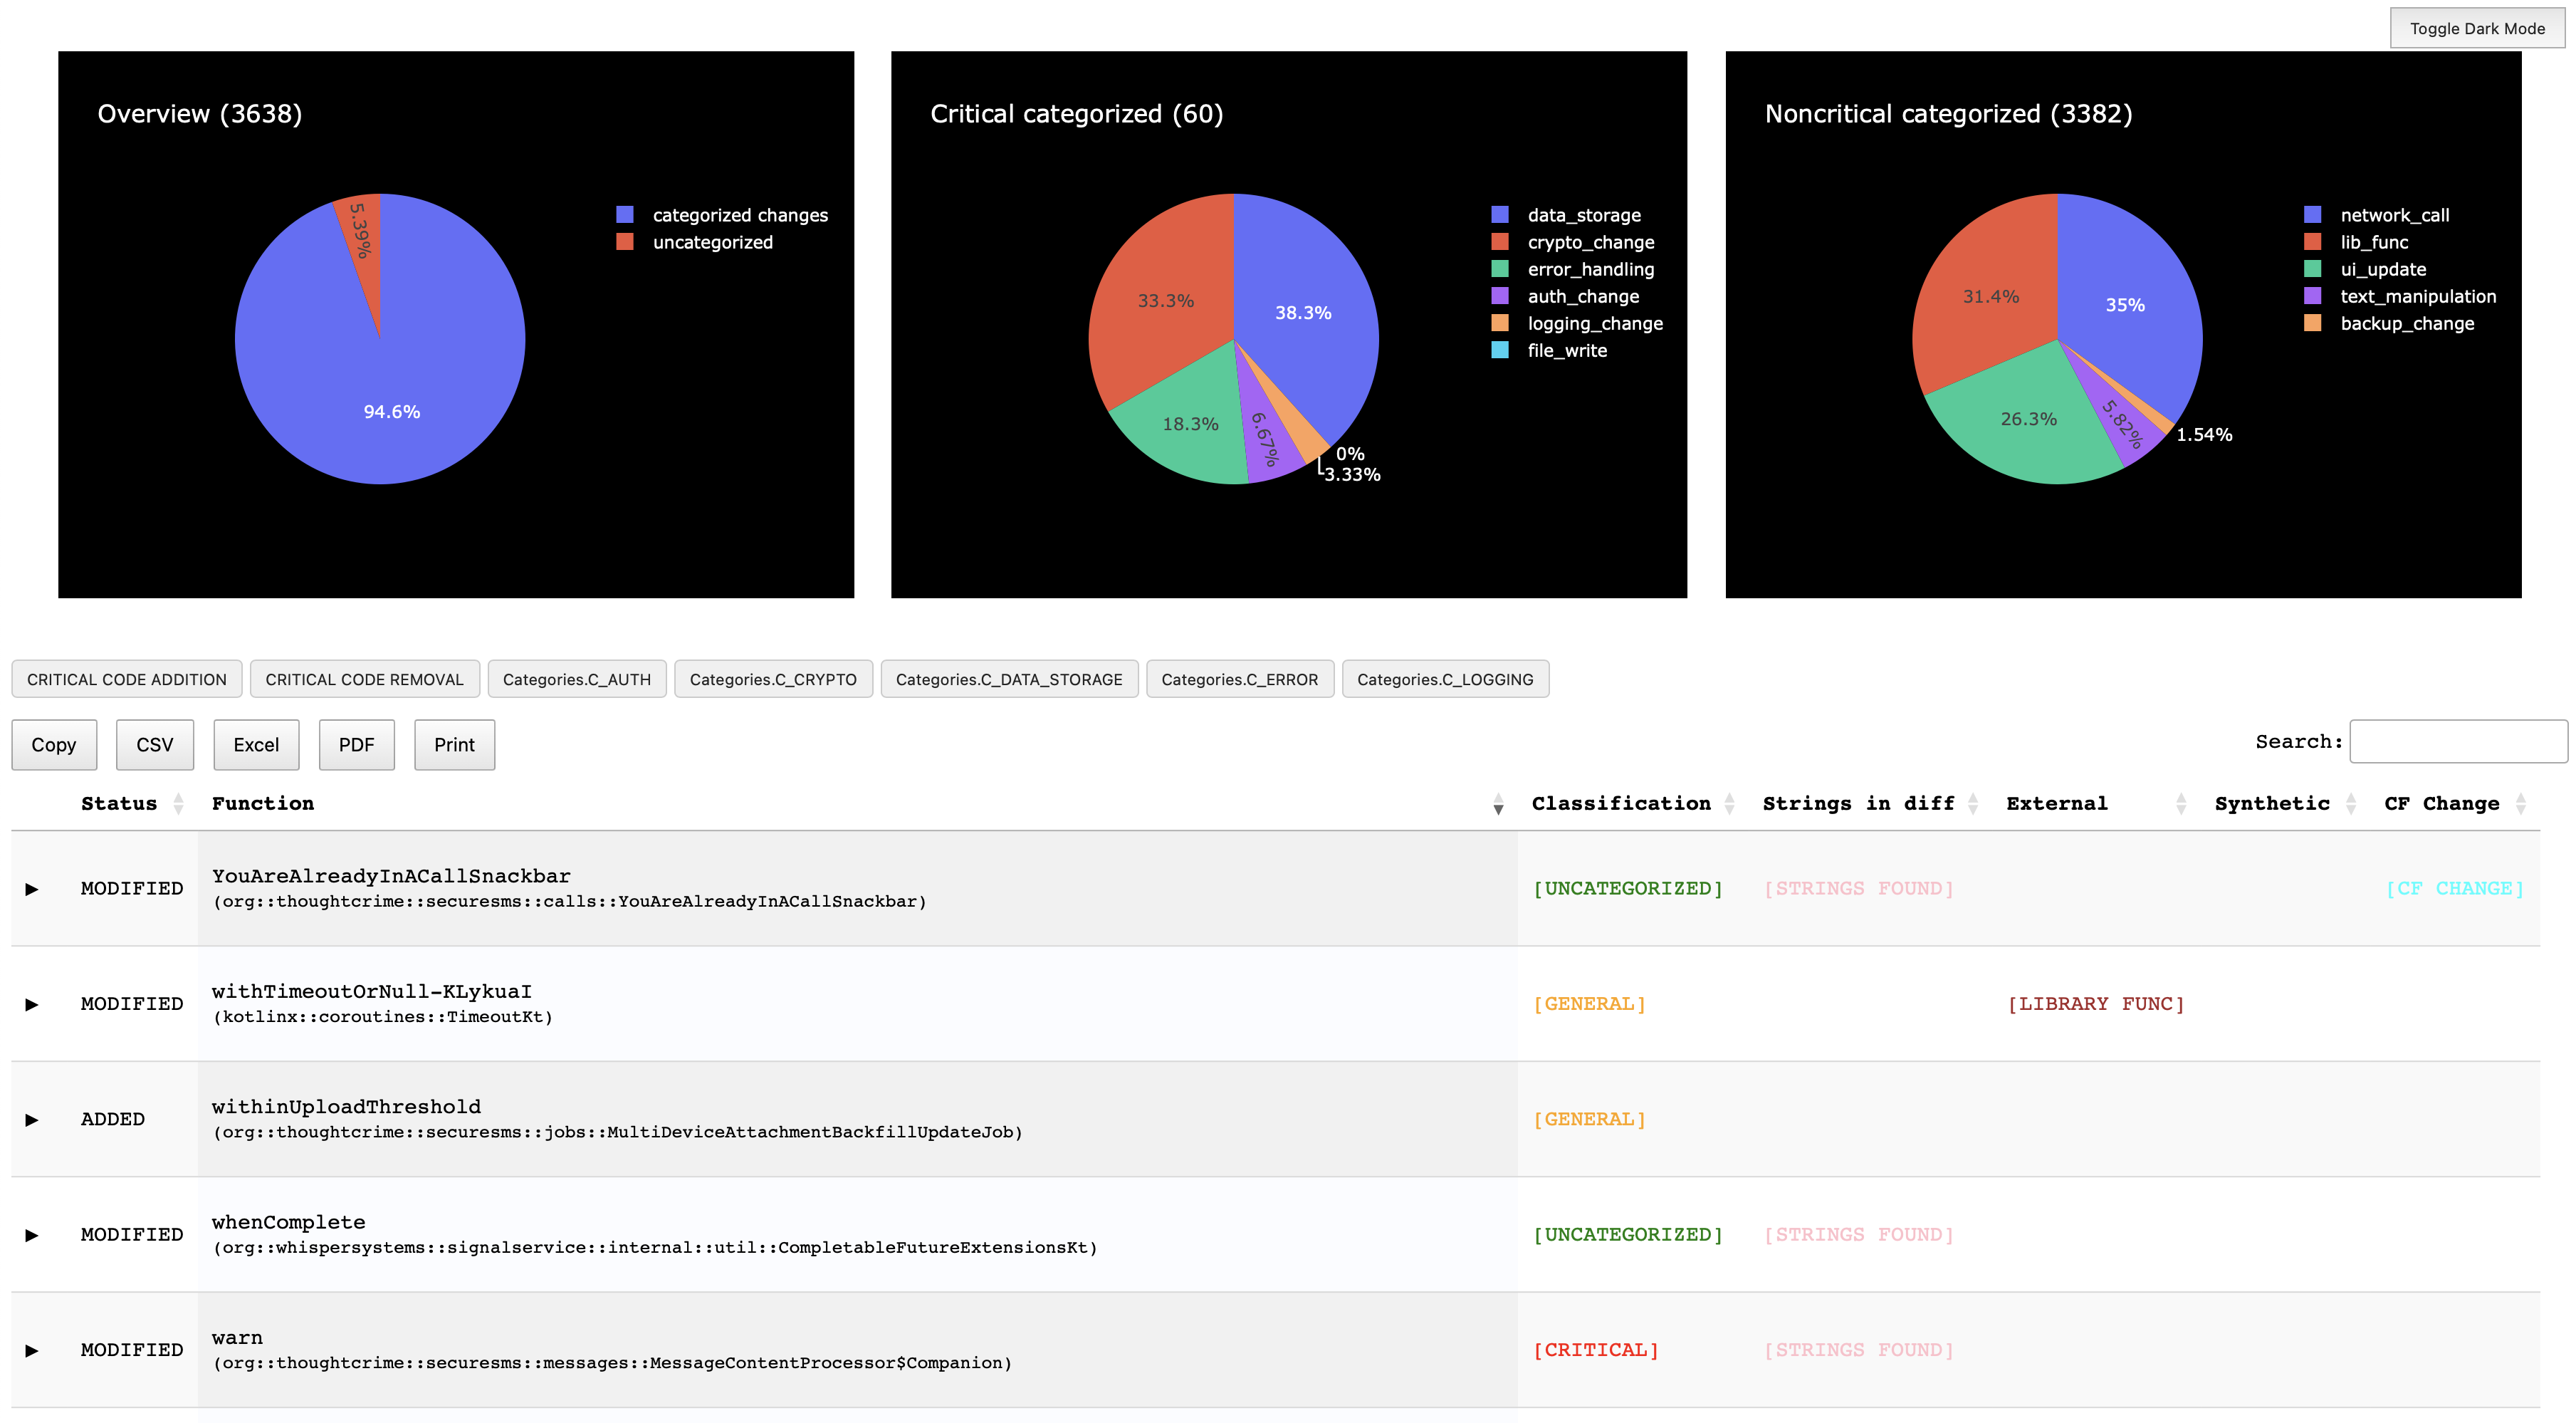
\includegraphics[width=1\linewidth]{figures/results/report_screenshots/report_front_page.png}
    \caption{Screenshot of the HTML report front page}
    \label{fig:pipeline_frontpage}
\end{figure}

\begin{figure}
    \centering
    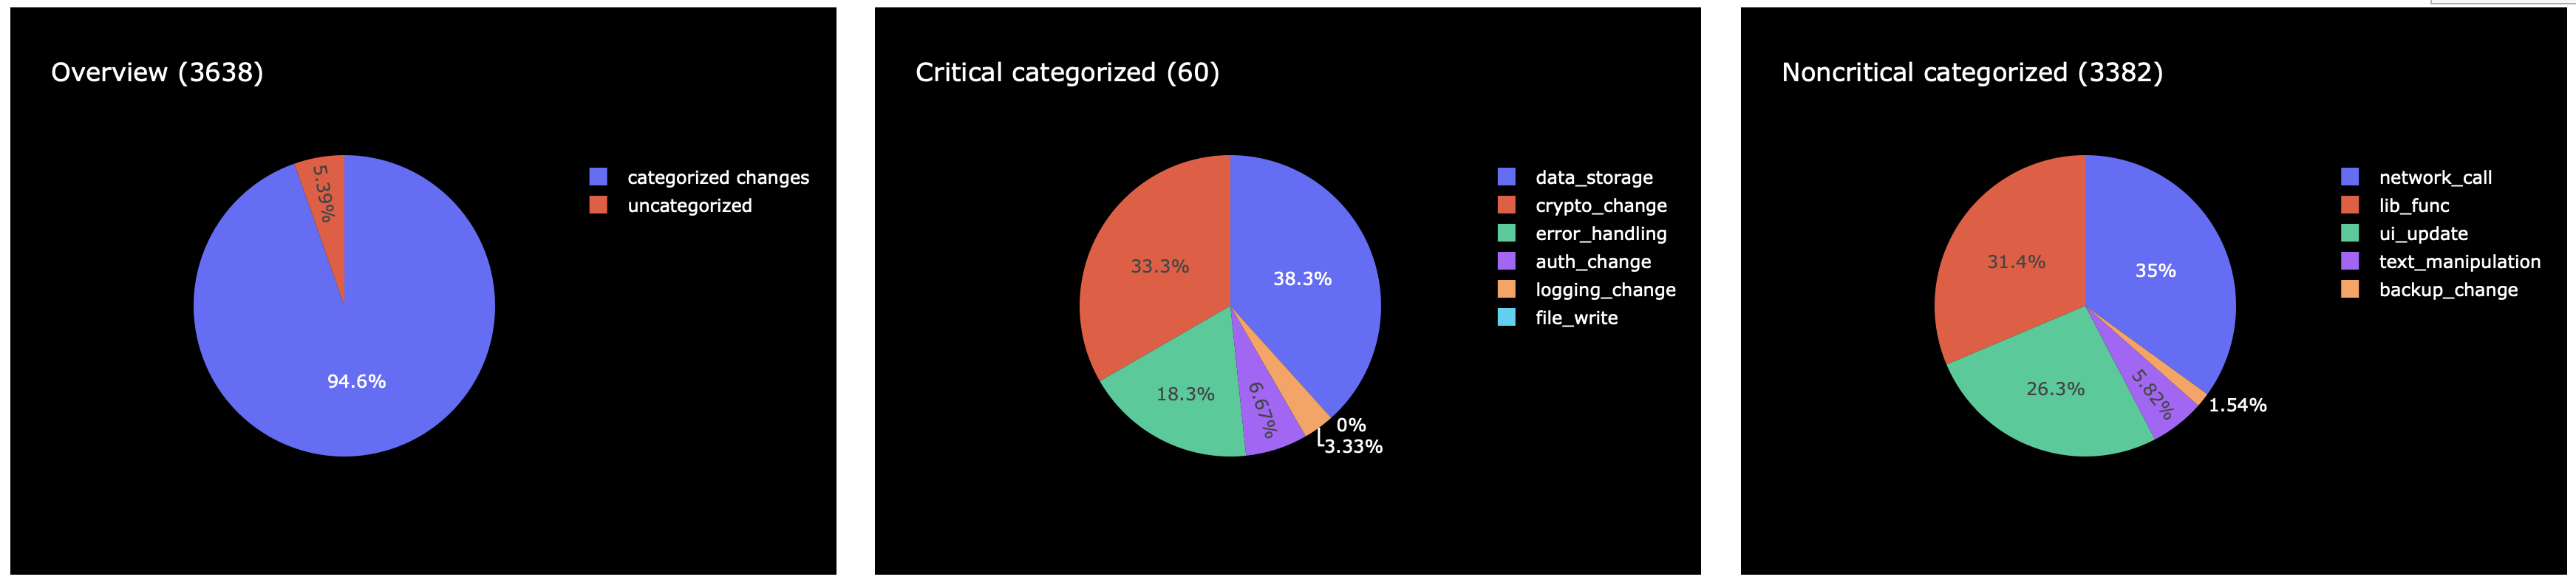
\includegraphics[width=1\linewidth]{figures/results/report_screenshots/diagrams.png}
    \caption{Screenshot of the pie charts showing the categorization and classification distributions}
    \label{fig:pipeline_piecharts}
\end{figure}

This section presents the HTML report generated by the tool after its analysis. The generated report provides a detailed view of the analysis results, including key features and layout elements. Each feature is explained in a dedicated subsection, describing its functionality. The data in the figures is purely illustrative and should be regarded as an example of the report's format and content.

Figure \ref{fig:pipeline_frontpage} illustrates the full-width front page of the HTML report. At the top of this report, three pie charts provide a visual summary of the categorization results generated by the pipeline. A more focused view of these pie charts is presented in Figure \ref{fig:pipeline_piecharts}, offering a closer look at the distribution of categorized changes.


Figure \ref{fig:pipeline_filtering_categories} presents the category filtering section of the HTML report. This section is designed to help users explore and analyze the changes detected in the analyzed software versions. Each button in this section represents a category identified by the pipeline during the analysis process.

\begin{comment}
These categories are used to classify the detected changes based on their nature and impact. They are broadly divided into two types: critical and non-critical categories. Critical categories include changes that directly affect the application's core functionality, security, or data handling. Examples of critical categories are data storage changes, which involve modifications in how data is read, written, or stored; authentication changes, which affect login mechanisms, session management, or token validation; cryptographic changes, which involve updates to encryption algorithms, key management, or hashing techniques; and file write changes, which relate to modifications in file-writing processes, such as creating, modifying, or deleting files.
\end{comment}

\begin{figure}
    \centering
    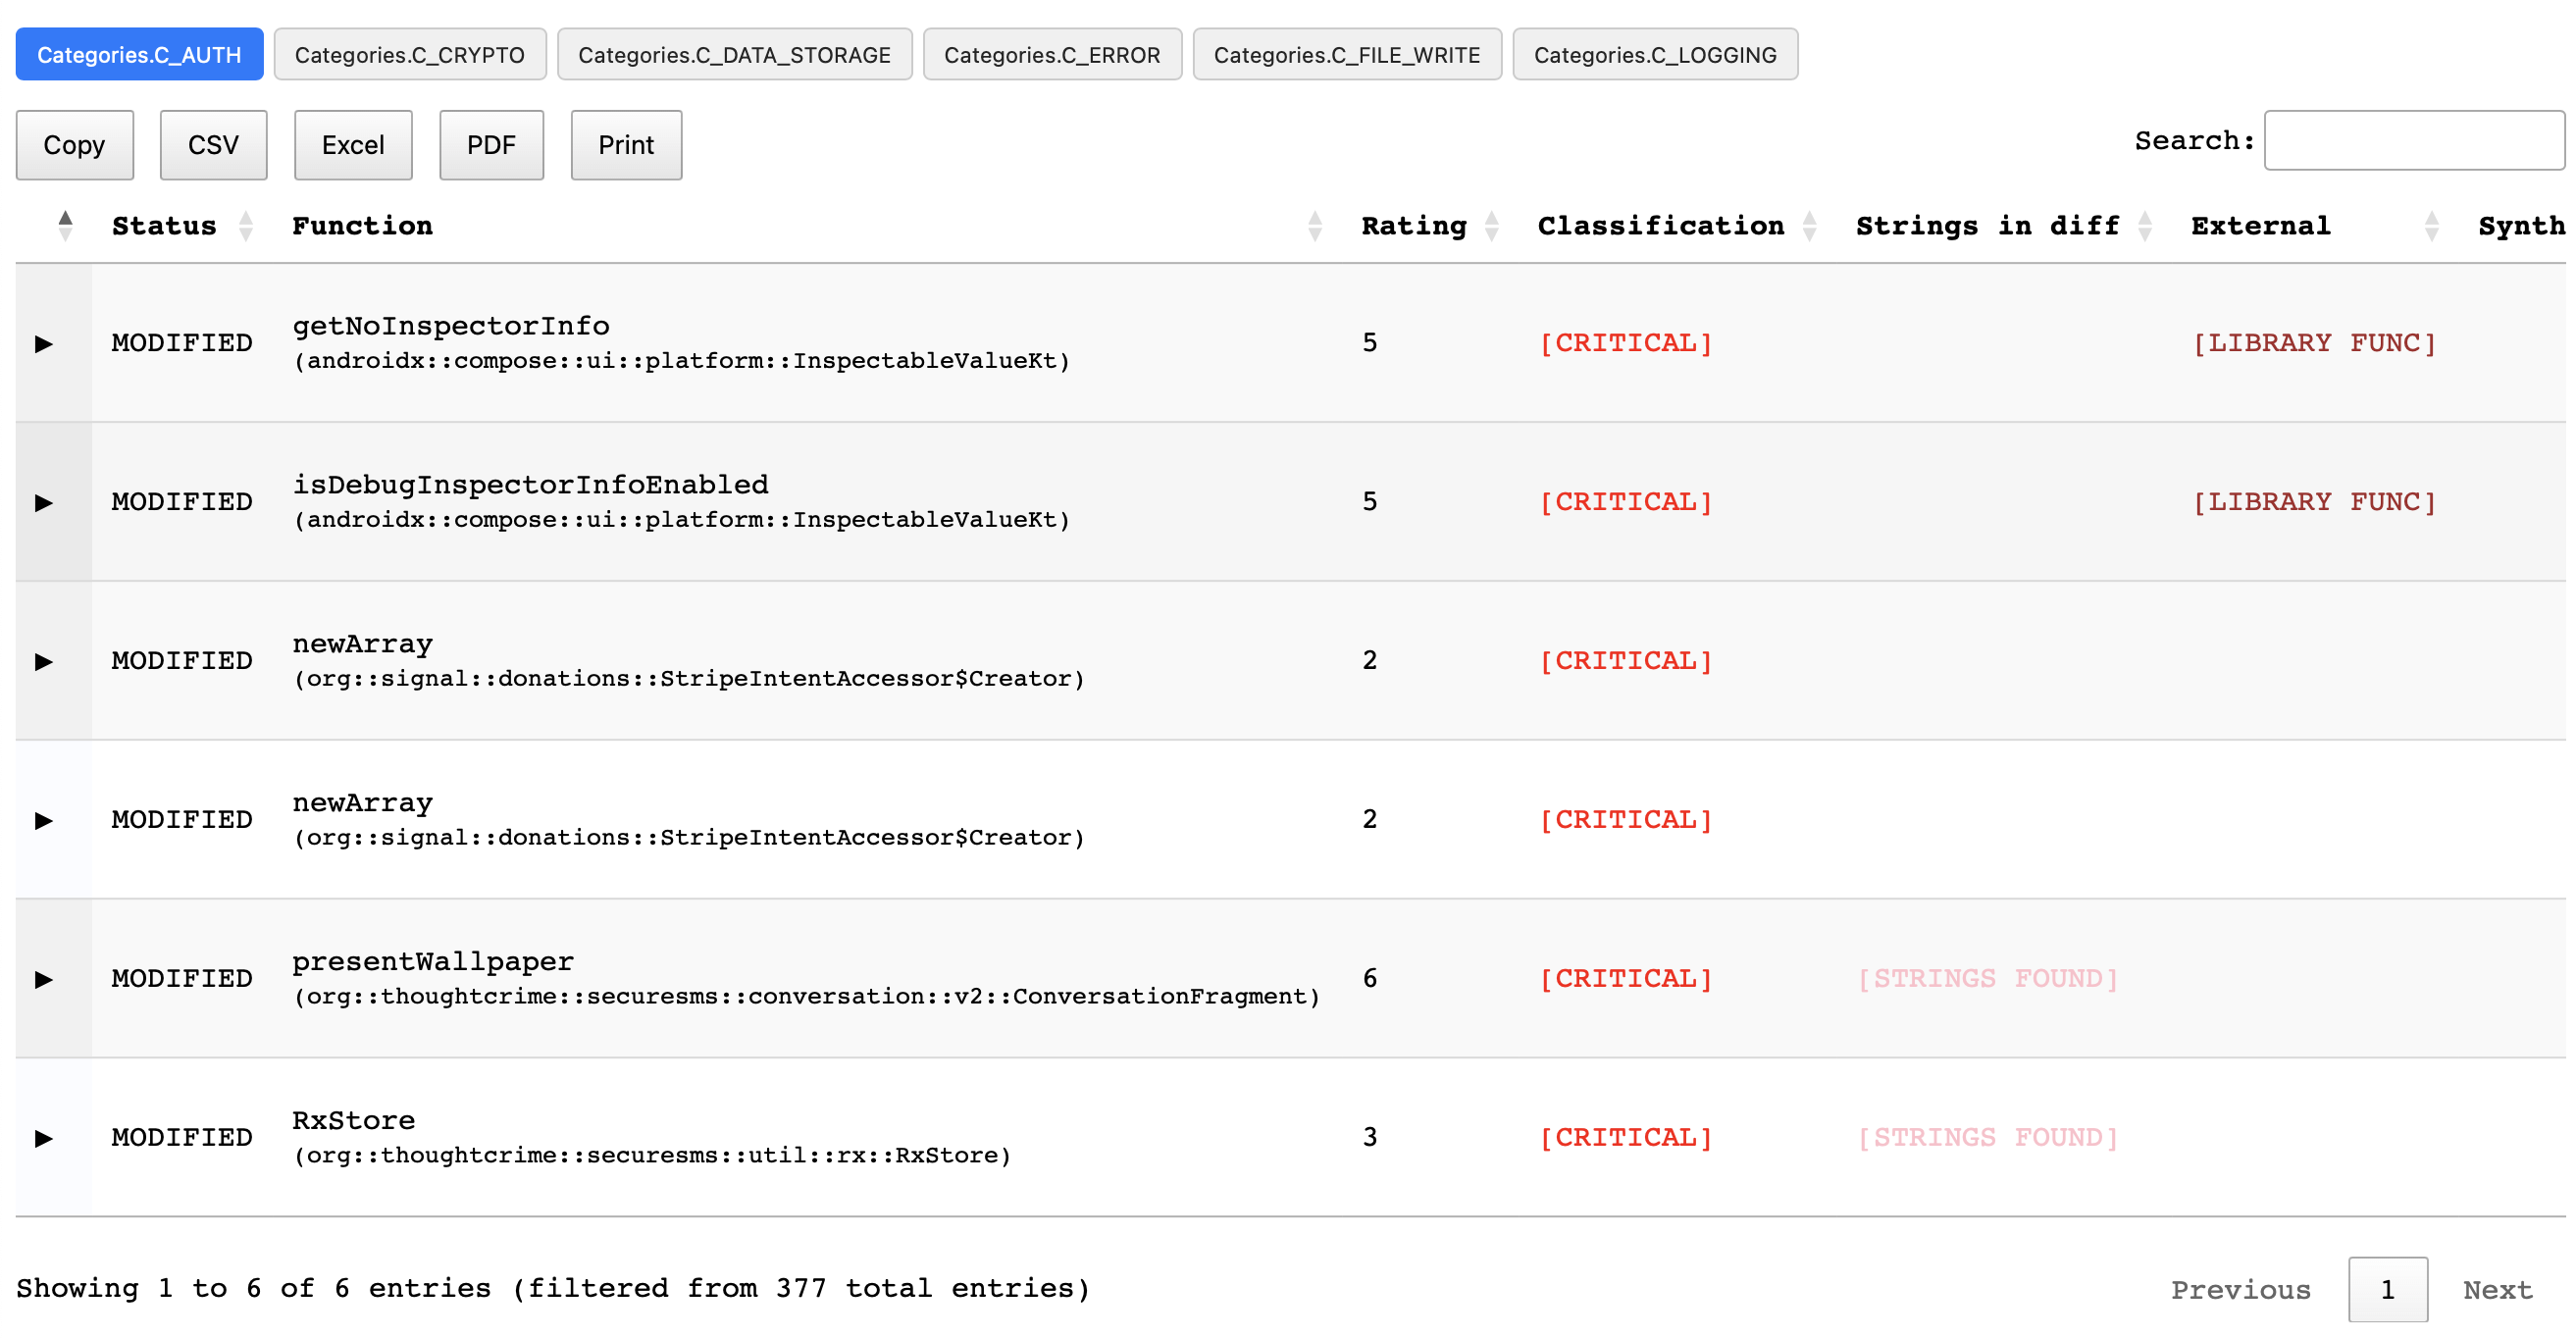
\includegraphics[width=1\linewidth]{figures/results/report_screenshots/feature_filtering.png}
    \caption{Filtering on changes which has been defined as Authentication handling}
    \label{fig:pipeline_filtering_categories}
\end{figure}

\begin{comment}
Non-critical categories, on the other hand, capture less impactful but still relevant changes, such as UI updates (alterations in user interface elements like layouts and colors), network calls (changes in API requests, endpoints, or response handling), and library functions (updates to external libraries or imported functions).
\end{comment}

By clicking on any of these category buttons, users can filter the displayed changes to focus only on those matching the selected category. Multiple categories can be selected simultaneously, with the filter combining them to provide a flexible and precise view of the categorized changes. This filtering system allows users to quickly identify and focus on the most relevant modifications, streamlining the analysis process.


Figure \ref{fig:pipeline_exporting} illustrates the export feature of the HTML report, positioned on the left side of the page. This section provides a set of buttons, each representing a different method for exporting the tabular data displayed in the report. Users can choose from various export formats, such as CSV, Excel, or PDF, allowing them to save the analyzed data for offline review or further analysis. It is important to note that this export functionality is limited to the data shown in the table and does not include the graphical diagrams or charts presented in the report. This separation ensures that users can efficiently export only the detailed, categorized results they are interested in.

\begin{figure}
    \centering
    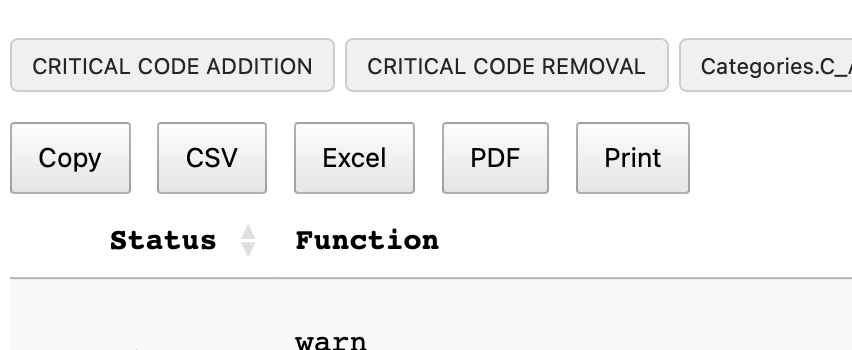
\includegraphics[width=0.5
    \linewidth]{figures/results/report_screenshots/feature_exporting.png}
    \caption{Exporting capabilities for data shown in tabular}
    \label{fig:pipeline_exporting}
\end{figure}

The HTML report provides a search field located next to the export buttons, making it easy for users to quickly find specific information. By entering a search term, users can filter the table, showing only the rows where the search term appears. For example, if you search for a function name or part of a file path, only rows matching that term will be displayed, while everything else is hidden. This feature, shown in Figure \ref{fig:pipeline_searchfield}, helps users focus on the most relevant data.

Just below the export buttons and the search field is the main data table. This table is organized in a simple row-and-column format, where each row represents a detected change, and each column shows details about that change, such as its category, function name, and other information. 

\begin{comment}
The layout makes it easy to review and understand the results and is presented in Figure \ref{fig:pipeline_datatable}.
\end{comment}

\begin{figure}
    \centering
    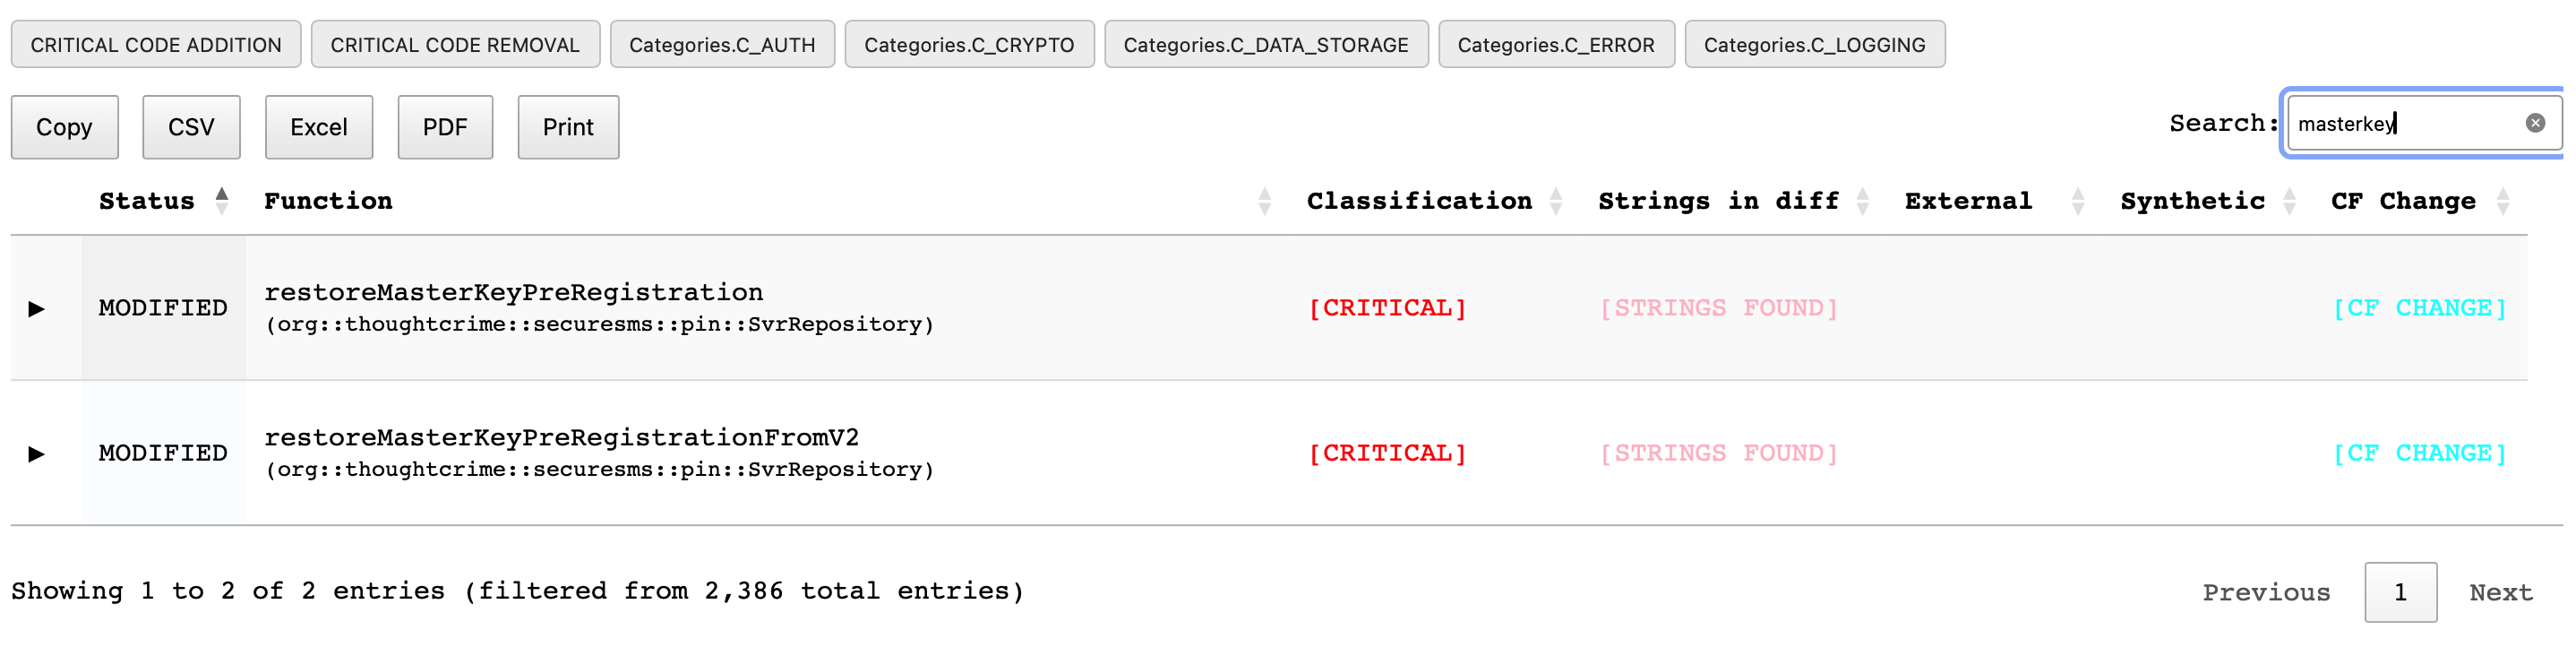
\includegraphics[width=1\linewidth]{figures/results/report_screenshots/feature_search.png}
    \caption{Searching for 'masterkey', which looks at the value of the \textit{Function} column}
    \label{fig:pipeline_searchfield}
\end{figure}



\begin{comment}
\begin{figure}
    \centering
    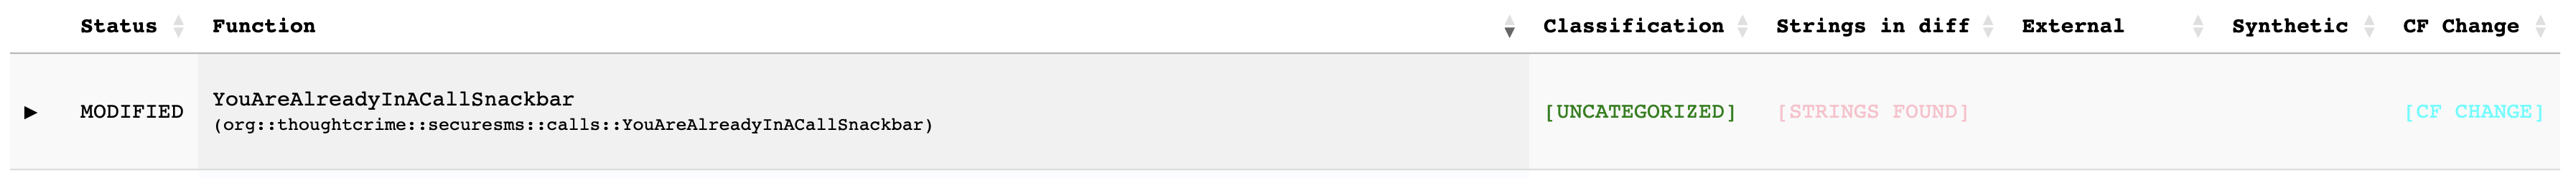
\includegraphics[width=1\linewidth]{figures/results/report_screenshots/table_columns.png}
    \caption{Caption}
    \label{fig:pipeline_datatable}
\end{figure}
\end{comment}


\begin{figure}
    \centering
    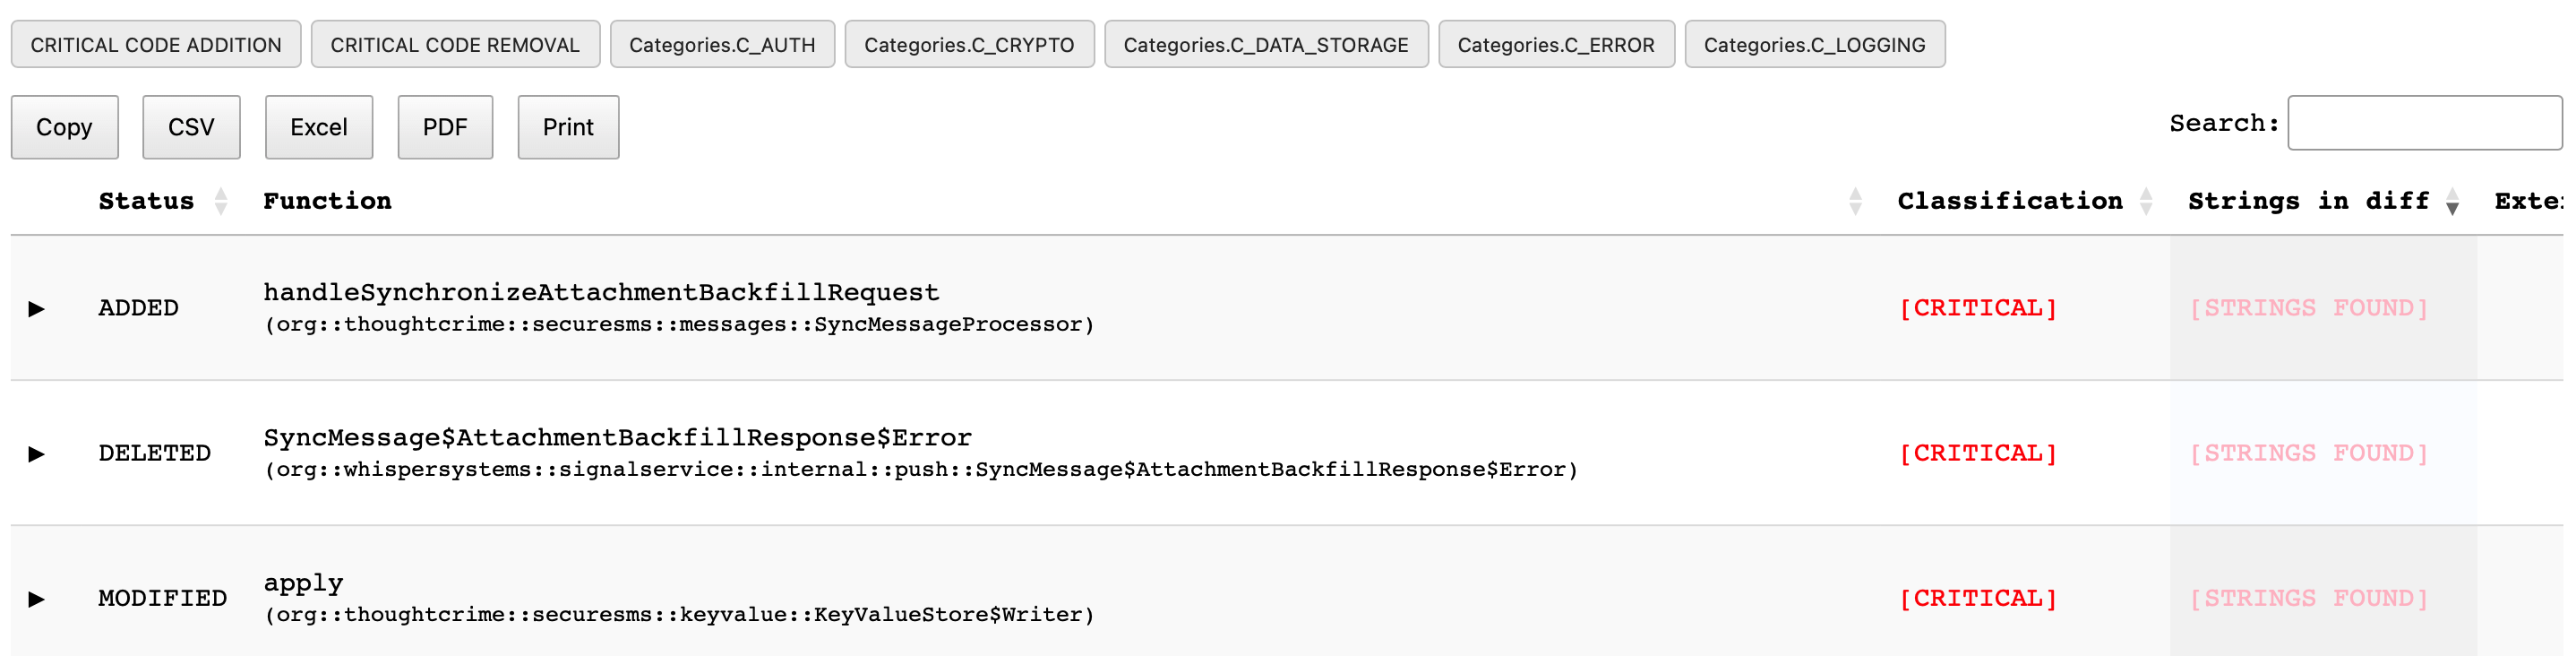
\includegraphics[width=1\linewidth]{figures/results/report_screenshots/feature_sorting1.png}
    \caption{Sorting on \textit{Classification} and \textit{Strings in diff}}
    \label{fig:pipeline_sorting_1}
\end{figure}

\begin{figure}
    \centering
    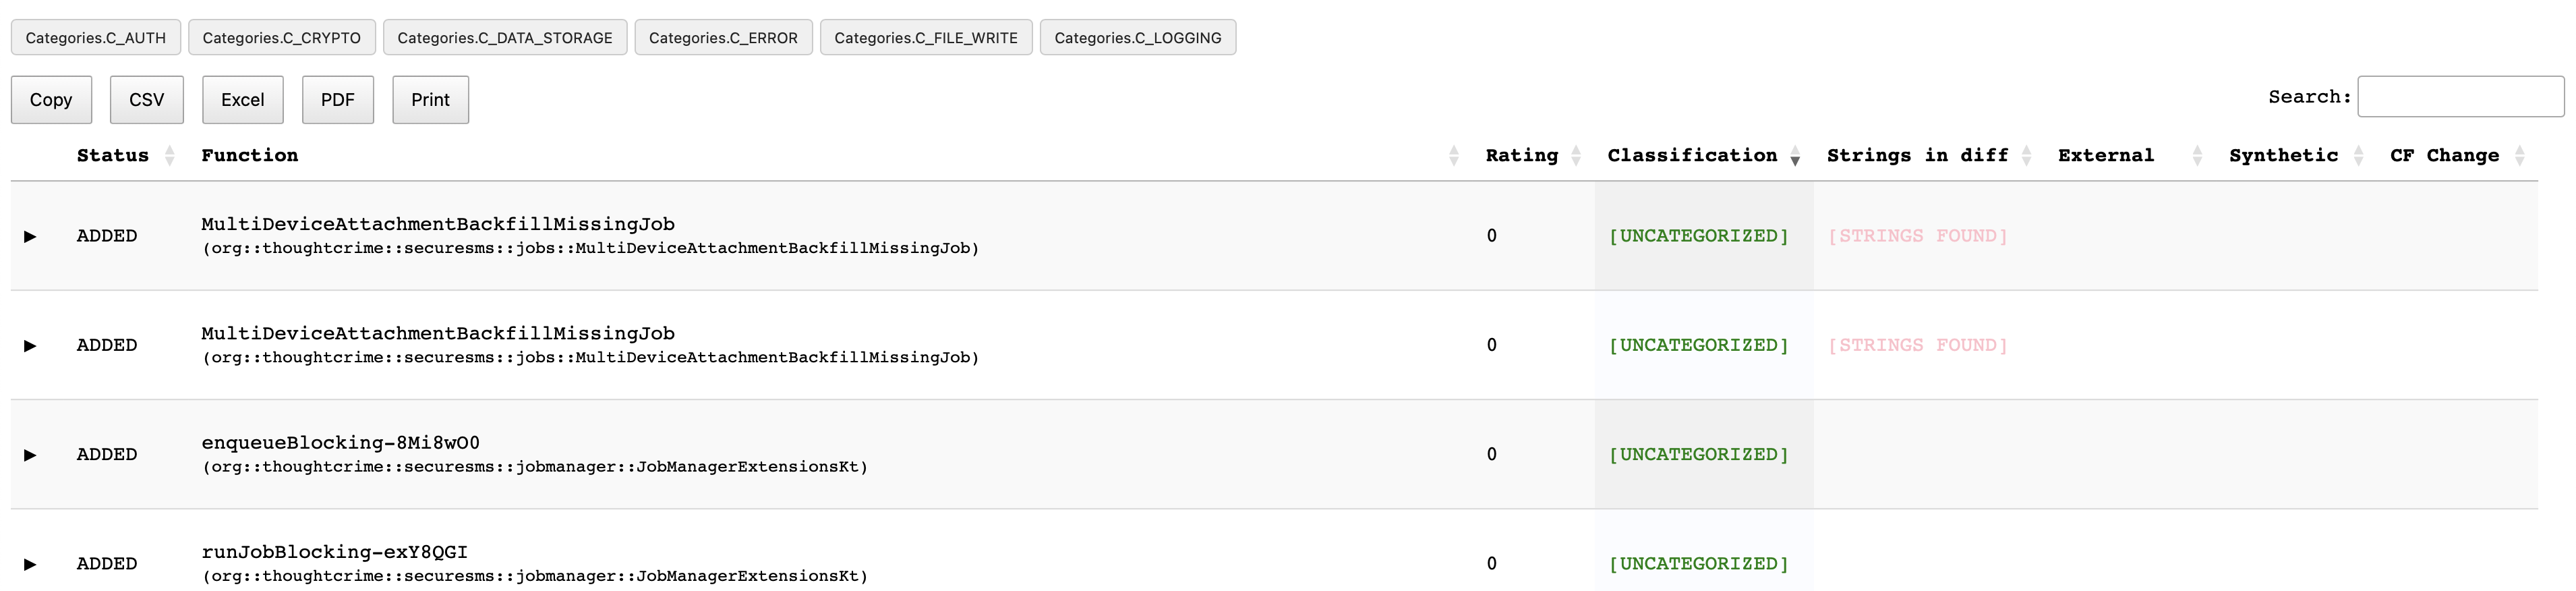
\includegraphics[width=1\linewidth]{figures/results/report_screenshots/feature_sorting2.png}
    \caption{Sorting on \textit{Function status} and \textit{Classification}}
    \label{fig:pipeline_sorting_2}
\end{figure}

The HTML report’s data table offers flexible sorting and detailed viewing options, making it easier for users to explore and analyze the detected changes. Users can sort the table by clicking on any column name, which immediately rearranges the rows based on the values in that column. For example, clicking on the Category column will sort the entries alphabetically by category. Moreover, the report supports multi-level sorting—users can achieve this by clicking multiple column names in sequence, allowing for more precise data organization. This functionality is illustrated in Figures \ref{fig:pipeline_sorting_1} and \ref{fig:pipeline_sorting_2}, which show two different sorting configurations.

Beyond sorting, the table provides an expandable row feature for in-depth analysis. Each row can be expanded to display additional information about the corresponding change, offering insights beyond the basic data shown in the main table. This detailed view reveals extra data collected during the change detection and categorization process, helping users better understand the nature of each modification. Figures \ref{fig:pipeline_detailedview1} and \ref{fig:pipeline_detailedview2} provide visual examples of how this expanded information is presented.

\begin{figure}
    \centering
    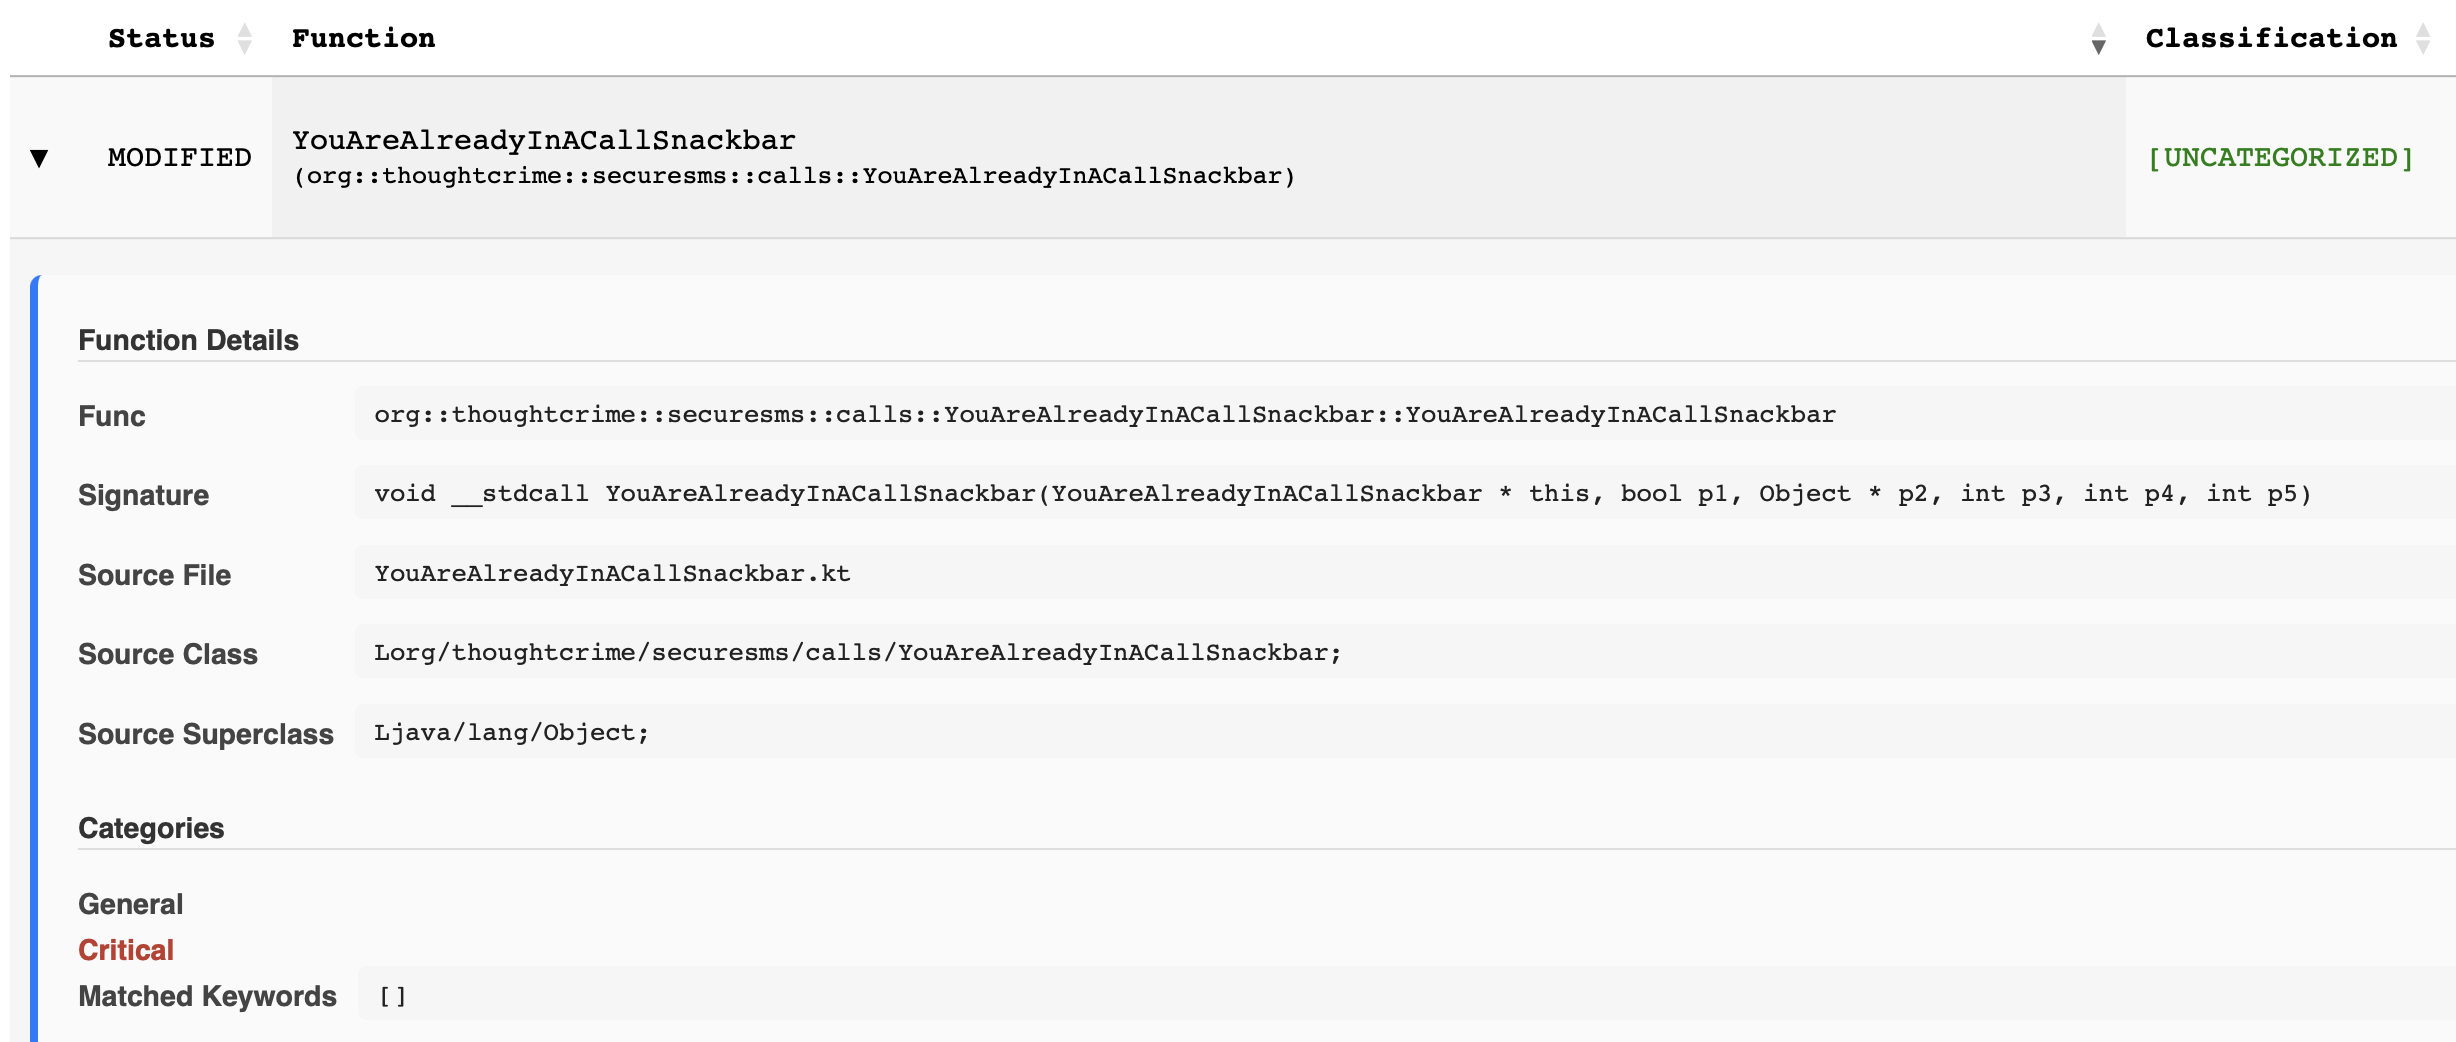
\includegraphics[width=1\linewidth]{figures/results/report_screenshots/method_detailed_1.png}
    \caption{Detailed view of a single change}
    \label{fig:pipeline_detailedview1}
\end{figure}

\begin{figure}[H]
    \centering
    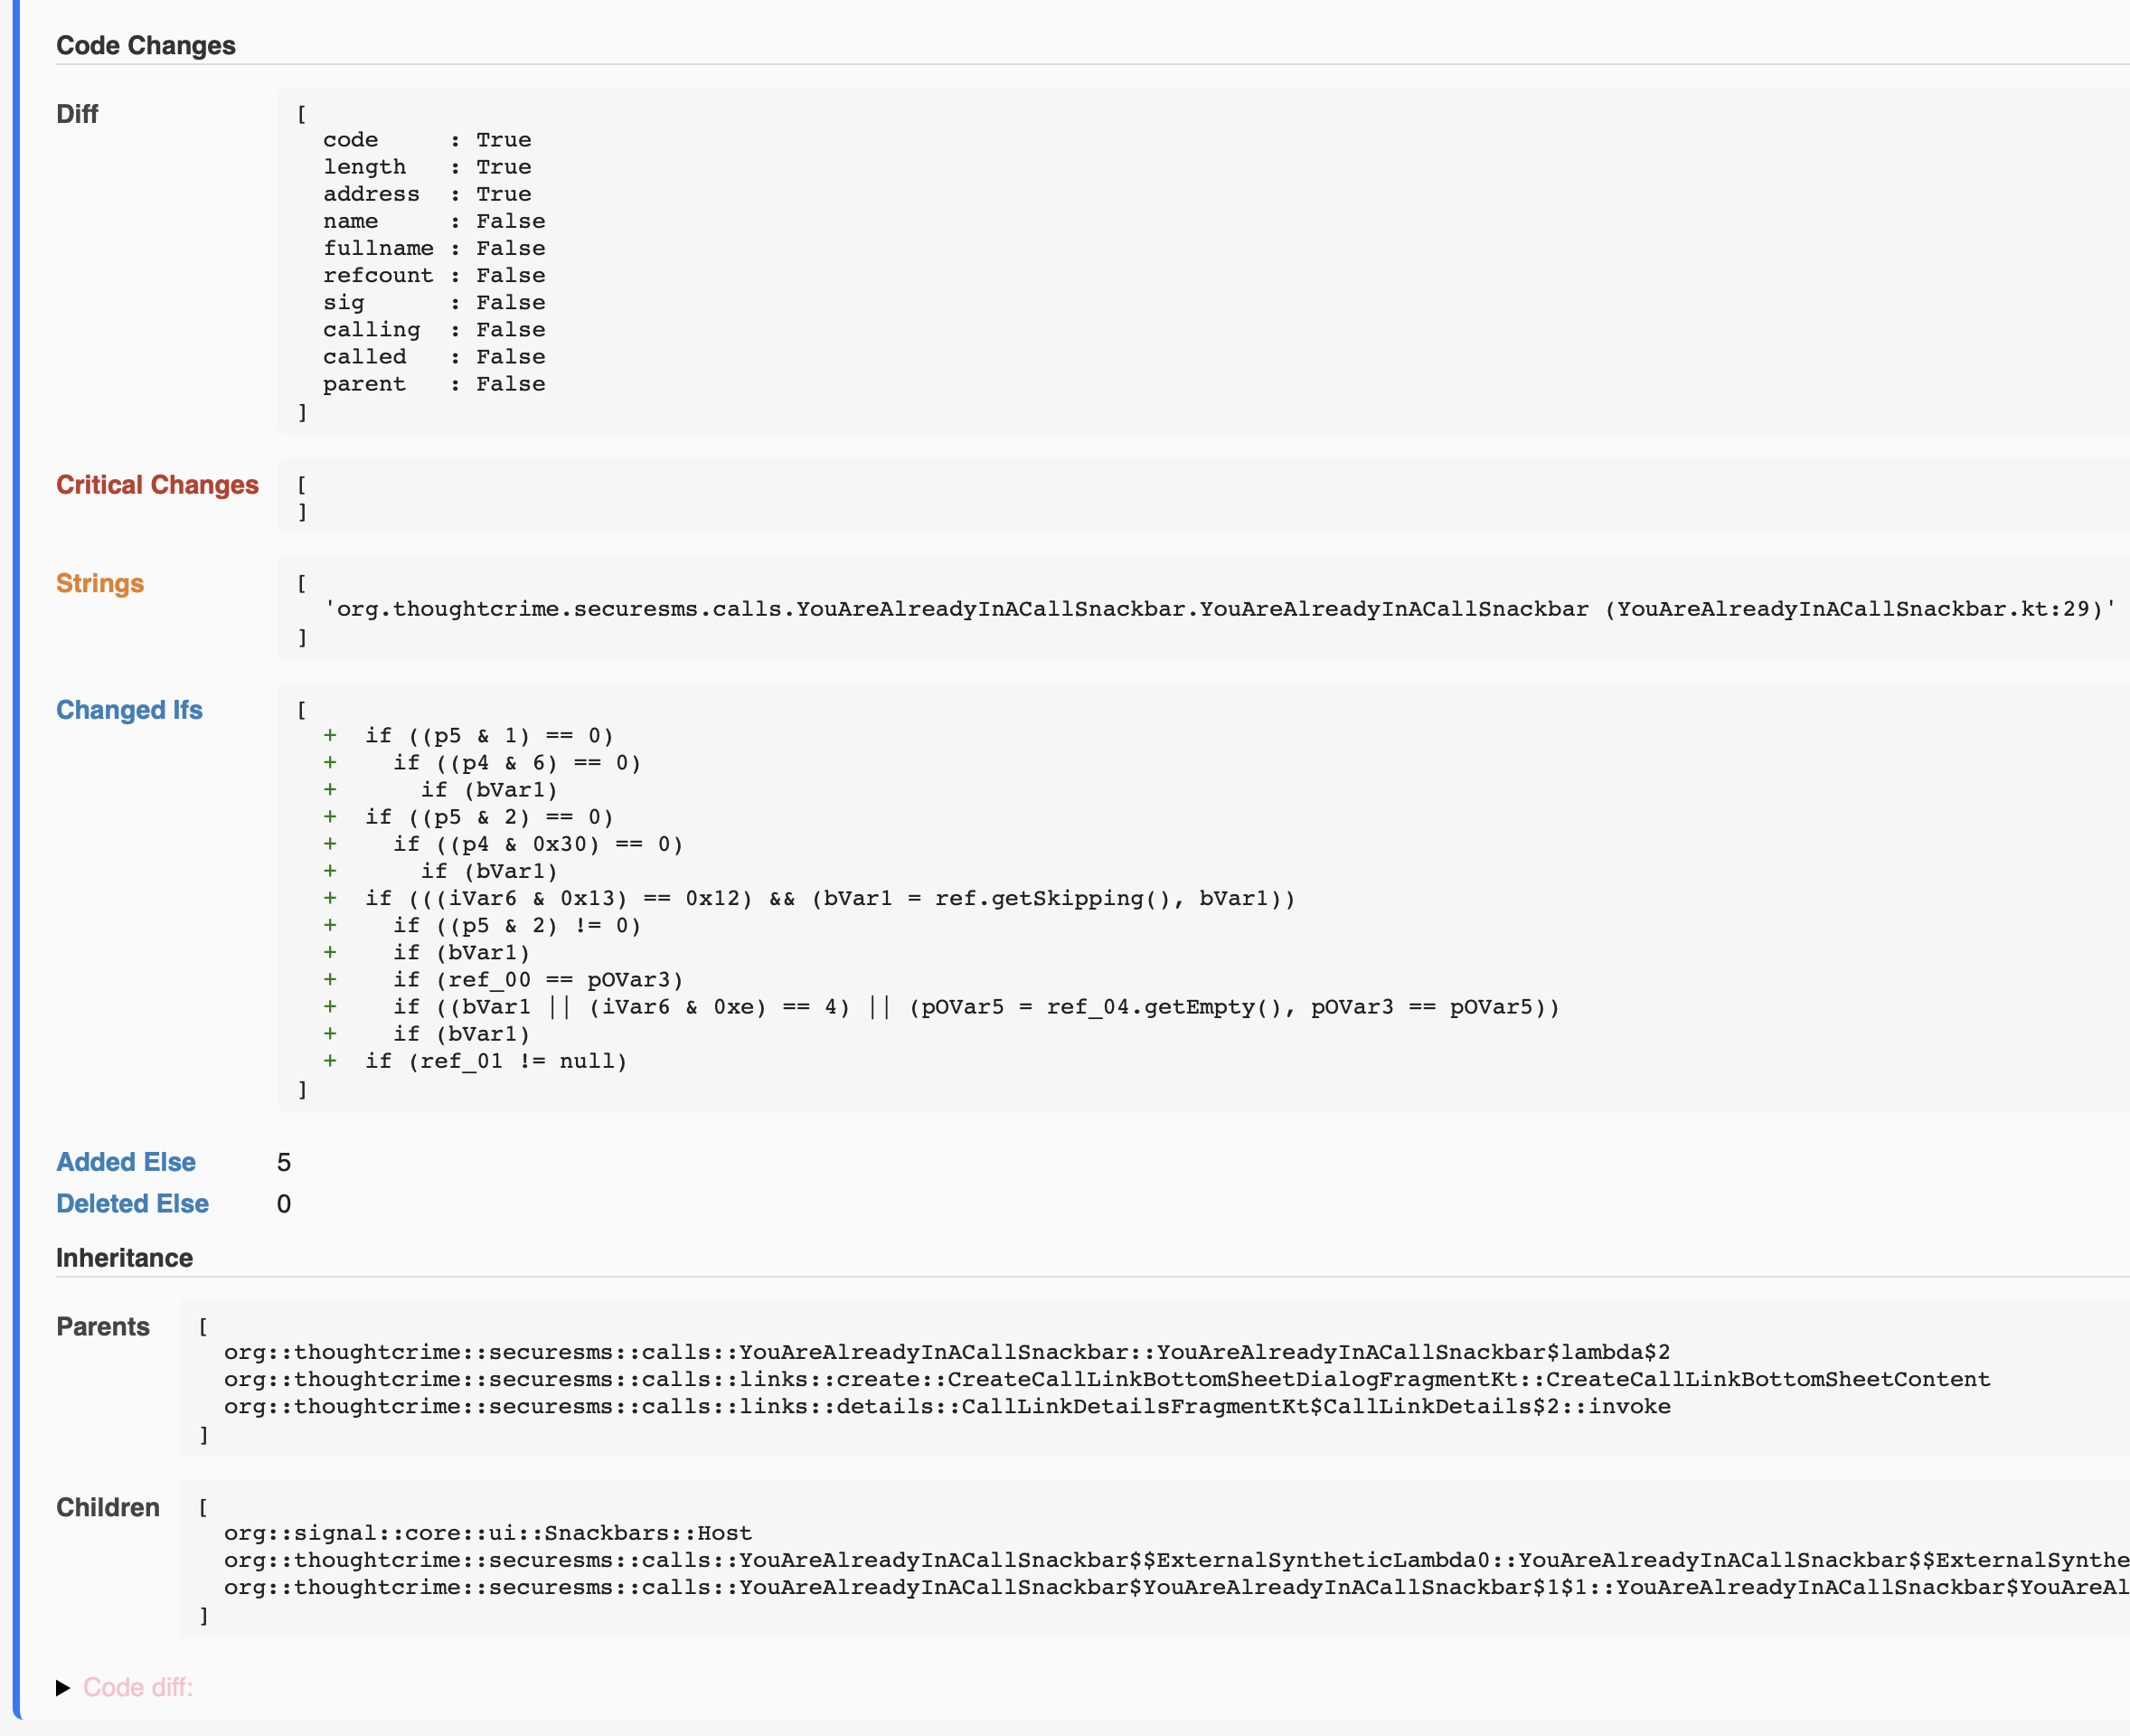
\includegraphics[width=1\linewidth]{figures/results/report_screenshots/method_detailed_2.png}
    \caption{Continued detailed view of a single change}
    \label{fig:pipeline_detailedview2}
\end{figure}

The HTML report offers a feature for comparing decompiled Ghidra code, providing a view of changes between the "old" and "new" versions of the analyzed binaries. This comparison is accessible directly within the detailed view of each detected change. The code differences are highlighted using color coding—the "old" version appears in red, while the "new" version is in green. This visual contrast makes it easy to identify added, removed, or modified lines of code, providing a clear understanding of how the code has changed. Figure \ref{fig:pipeline_codecomparison} demonstrates this code comparison feature.

The report also includes a dark mode option, which can be toggled using a button at the top of the page, and Figure \ref{fig:pipeline_darkmode} presents an example of the report displayed in dark mode.

\begin{figure}[H]
    \centering
    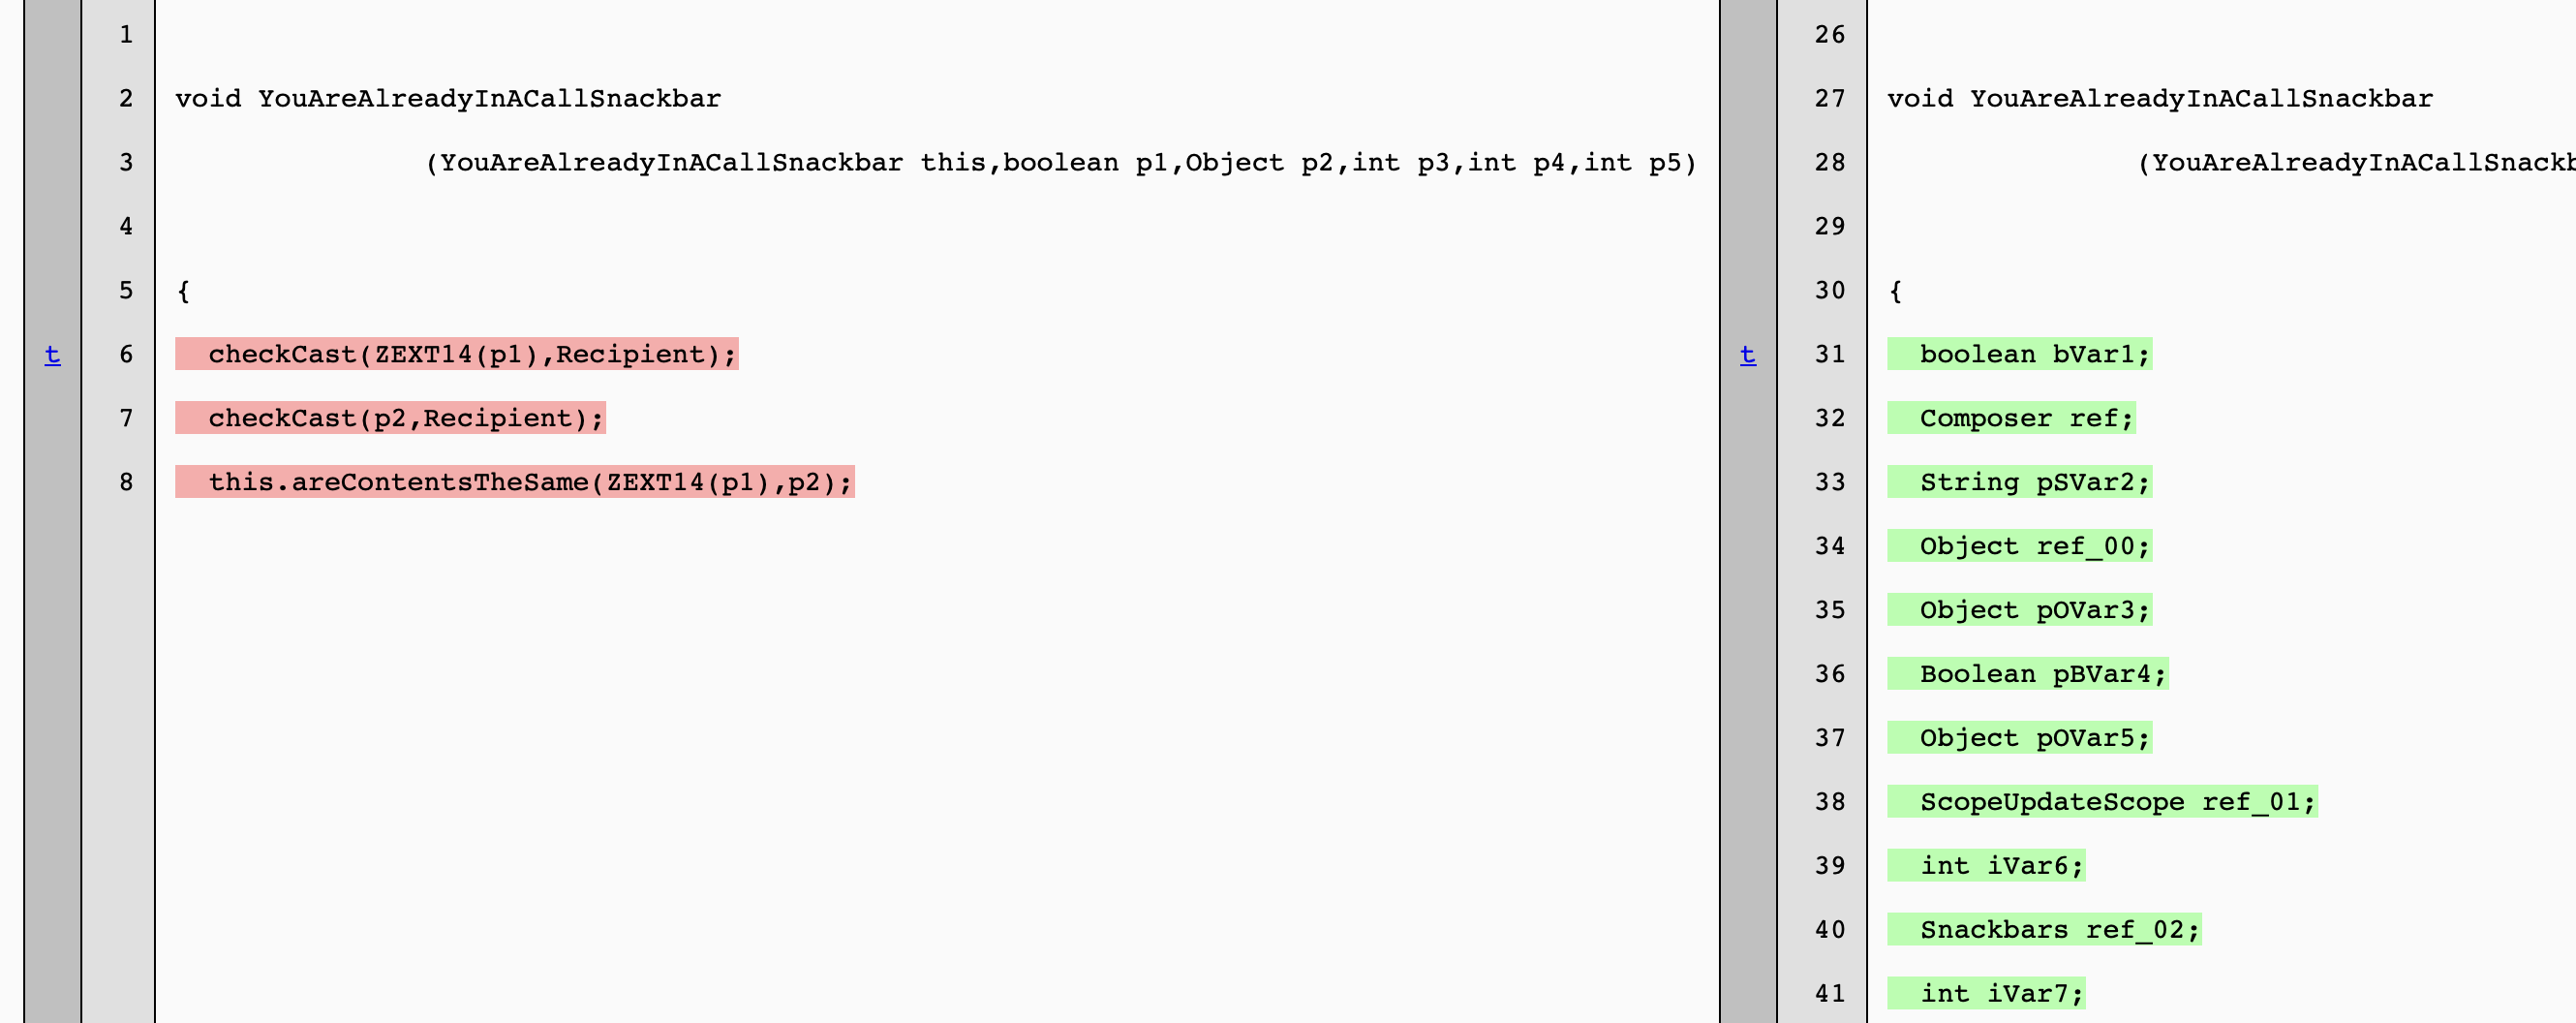
\includegraphics[width=1\linewidth]{figures/results/report_screenshots/method_detailed_code_comparison.png}
    \caption{Decompiled Ghidra code comparison}
    \label{fig:pipeline_codecomparison}
\end{figure}

\begin{figure}[H]
    \centering
    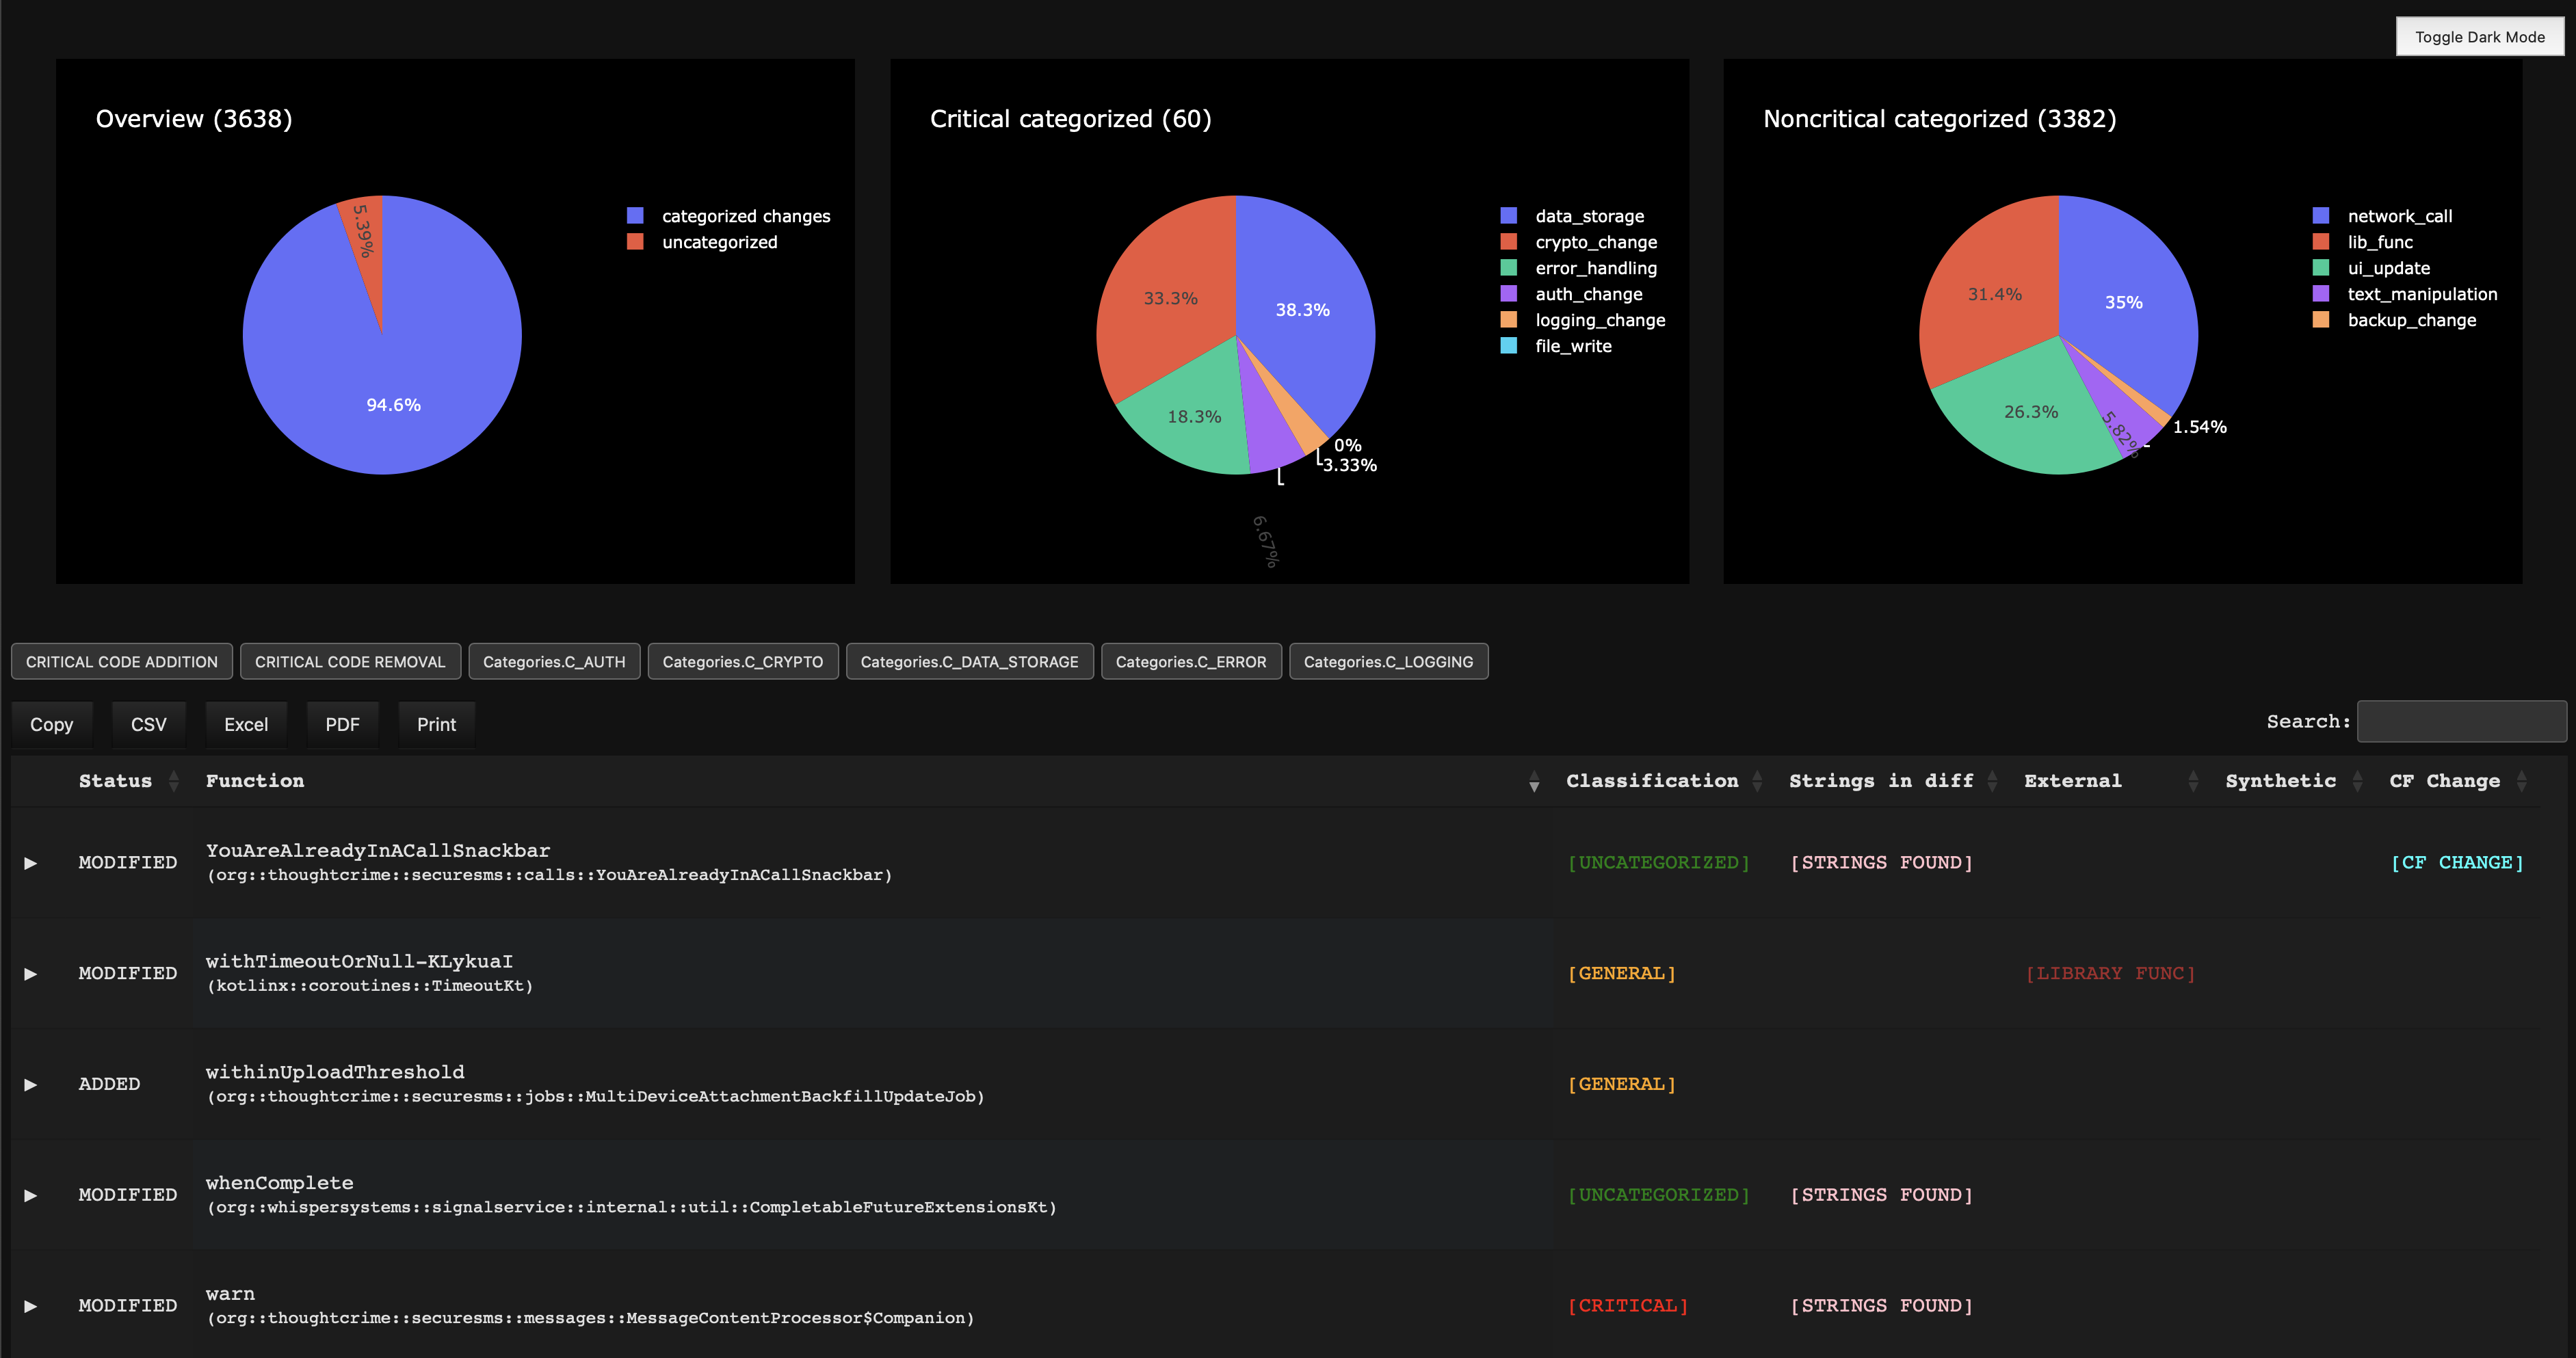
\includegraphics[width=1\linewidth]{figures/results/report_screenshots/feature_darkmode.png}
    \caption{Darkmode enabled}
    \label{fig:pipeline_darkmode}
\end{figure}


\newpage
\section{Categorization Results}
This section presents the results obtained from analyzing three different versions of the Signal Android application using the tool developed in this thesis. The selected versions, summarized in Table \ref{tab:release_overview}, are sourced from Signal's official Android GitHub repository \cite{githubSignal}. Additionally, Table \ref{tab:run_time} provides an overview of the tool’s runtime performance for each version analysis, including key metrics such as analysis duration and the number of detected changes.

\begin{note}
    Partial Analysis of Version Diff B\\
    \noindent
    For version diff B, only a subset of the GitHub changes was manually reviewed during the analysis. Consequently, while Table \ref{tab:run_time} lists a higher number of detected changes for version diff B compared to version diff A, the actual volume of analyzed result data presented in this chapter is smaller for version diff B. This discrepancy is due to the limited scope of the manual review.
\end{note}


\subsection{Understanding the Pipeline Analysis}
The pipeline analysis in this section focuses on three key aspects:

\begin{description}
    \item[Change Detection] Identifying individual changes between the two versions of the Signal application. Each change is defined as a single method-level modification detected between the compared versions.

    \item[Status Classification] Assigning each detected change to one of three status categories: Critical, Non-critical, or Uncategorized. These categories help determine the significance of each change.

    \item[Functional Categorization] Labeling each detected change with one or more functional categories, such as \codebox{Data storage}, \codebox{UI update}, or \codebox{Authentication}. Unlike the status classification, a single change can belong to multiple functional categories.
\end{description}

It is important to note that the total number of detected changes reflects the unique modifications found, while the count of changes in each category may exceed this total because some changes are assigned to multiple categories. This distinction ensures a clear understanding of the results and their classification.

\begin{table}[H]
  \centering
  \begin{tabular}{@{} c c c c c c c @{}}
    \toprule
    \textbf{Version diff} & \textbf{Base} & \textbf{Target} & \textbf{Release date} & \textbf{Commits} & \textbf{File changed} \\ \midrule
    A & v7.30.2 & v7.31.0 & 2025-01-23 & 46 & 171 \\
    B & v7.34.2 & v7.35.0 & 2025-02-21 & 33 & 173 \\
    C & v7.40.0 & v7.40.1 & 2025-04-11 & 12 & 85 \\ \bottomrule
  \end{tabular}
  \caption{Overview of version diffs from Signal's Android GitHub repository \cite{githubSignal}}
  \label{tab:release_overview}
\end{table}


\begin{note}
    Failed .dex File Analysis.\\
    \noindent
    The column labeled "Failed .dex files" in Table \ref{tab:run_time} indicates whether the pipeline (specifically Ghidra) encountered issues analyzing any .dex files. If any .dex files could not be properly analyzed, this can impact the accuracy of the results for that version diff. Missing or failed .dex file analysis reduces the likelihood of detecting all changes and can affect classification performance. This challenge is further discussed in Section \ref{sec:discussion-results}.
\end{note}


\begin{table}[H]
  \centering
  \begin{tabular}{@{} c c c c l @{}}
    \toprule
    \textbf{Version diff} & \textbf{Run time} & \textbf{Apk size} & \textbf{Detected changes} & \textbf{Failed .dex files} \\ \midrule
    A & 20m 45s & 99.3 MB  & 1677 &  \\
    B & 21m 43s & 100 MB & 2386 & classes2.dex \& classes5.dex \\
    C & 21m 25s & 102 MB & 377 & classes2.dex \\ \bottomrule
  \end{tabular}
  \caption{Runtime comparison of the different version diffs. Execution time captured on a MacBook Pro with M1 Pro chip}
  \label{tab:run_time}
\end{table}

\subsection{Manual Evaluation Process}
\label{sec:res:categorization_result:manual_evaluation_process}

To accurately assess the performance of the pipeline’s categorization, a manual evaluation process was conducted. This process involved carefully reviewing the source code for each version difference (diff) and comparing the results with the analysis generated by the pipeline. The manual evaluation followed these structured steps:

\begin{enumerate}
    \item \textbf{Identify Change Types:} For each detected change, it was determined whether it was an addition, modification, or deletion when comparing the new version of the code with the old version.

    \item \textbf{Assign Functional Categories:} Each identified change was categorized based on its nature and functionality. If a change matched any of the predefined functional categories (e.g., Data Storage, UI Update, Authentication), it was labeled accordingly. If none of the categories were applicable, the change was marked as \textit{Uncategorized}.

    \item \textbf{Compare with Pipeline Results:} Each manually identified change was cross-referenced with the HTML report generated by the pipeline. This comparison checked whether the pipeline correctly detected the change, accurately classified it, and assigned the appropriate categories. Any changes detected manually but missing from the pipeline report were also noted.
\end{enumerate}

The results of this manual evaluation are crucial because they serve as a benchmark for assessing the pipeline's accuracy. Although the manual analysis was conducted separately from the pipeline, it reflects the intended behavior of the tool and provides a standard for comparison. 


\subsection{Understanding Correct and Incorrect Classification}
\label{sec:result:understanding_correct_incorrect}
\begin{description}
    \item[Correct Category Classification] This means that the pipeline correctly assigned all categories identified during the manual analysis. Even if the pipeline assigned extra categories, it is still considered correct as long as it includes all the manually identified categories.

    \item[Incorrect Category Classification] This occurs when the pipeline fails to include all categories assigned during the manual analysis. This can happen if the pipeline detects only a subset of the manually assigned categories or if it entirely misses the correct categories.
\end{description}

Further discussion regarding the reliability of these manually gathered results can be found in Section~\ref{sec:discussion-results}.

\subsection{Pipeline Accuracy}

The accuracy of the pipeline’s categorization is determined by comparing its results with the manually reviewed source code analysis \cite{githubSignal}. This comparison helps measure how well the pipeline identifies changes, classifies them, and assigns appropriate categories. The results of this accuracy evaluation are summarized in Tables~\ref{tab:accuracy_A}, \ref{tab:accuracy_B}, and \ref{tab:accuracy_C}.

\noindent
The following metrics are used to evaluate pipeline accuracy:

\begin{description}
    \item[Changes Detected:] The proportion of changes in the source code that were correctly identified by the pipeline. It reflects how effectively the pipeline detects differences between software versions.

    \item[Correct Change Status:] The percentage of changes where the pipeline correctly identified the type of change (addition, modification, or deletion) as compared with the source code.

    \item[Correctly Set Categories:] The proportion of changes where the pipeline correctly assigned the same functional categories as those identified in the manual analysis. If the pipeline assigns all manually identified categories (even with additional categories), the classification is considered correct. However, if it assigns only a subset of the categories identified manually, the classification is marked as incorrect.
\end{description}

It is important to note that these accuracy metrics exclude any changes that the pipeline failed to detect due to limitations in Ghidriff's binary analysis capabilities. This ensures that the evaluation focuses solely on the changes that were actually detected.


\begin{table}[H]
    \centering
    \begin{tabular}{l l}
        \toprule
        \textbf{Metric} & \textbf{Accuracy} \\
        \midrule
        Changes detected & 96.4\% \\
        Correct change status & 84.5\% \\
        Correctly set categories & 85.7\% \\
        \textit{\ \ \ \ \ \ \ \ Critical categories} & 84.2\% \\
        \textit{\ \ \ \ \ \ \ \ Non-critical categories} & 88.9\% \\
        \bottomrule
    \end{tabular}
    \caption{Accuracy metrics for version diff A}
    \label{tab:accuracy_A}
\end{table}

\begin{table}[H]
    \centering
    \begin{tabular}{l l}
        \toprule
        \textbf{Metric} & \textbf{Accuracy} \\
        \midrule
        Changes detected                 & 75\% \\
        Correct change status            & 57.1\% \\
        Correctly set categories & 60.7\% \\
        \textit{\ \ \ \ \ \ \ \ Critical categories} & 56.25\% \\
        \textit{\ \ \ \ \ \ \ \ Non-critical categories} & 66.7\% \\
        \bottomrule
    \end{tabular}
    \caption{Accuracy metrics for version diff B}
    \label{tab:accuracy_B}
\end{table}

\begin{table}[H]
    \centering
    \begin{tabular}{l l}
        \toprule
        \textbf{Metric} & \textbf{Accuracy} \\
        \midrule
        Changes detected                 & 92.9\% \\
        Correct change status            & 82.1\% \\
        Correctly set categories & 53.6\% \\
        \textit{\ \ \ \ \ \ \ \ Critical categories} & 75\% \\
        \textit{\ \ \ \ \ \ \ \ Non-critical categories} & 50\% \\
        \bottomrule
    \end{tabular}
    \caption{Accuracy metrics for version diff C}
    \label{tab:accuracy_C}
\end{table}




%%%% Categorization distribution %%%%
\subsection{Categorization Distributions}

This section provides a detailed analysis of the distribution of categorized changes identified during the pipeline analysis. Specifically, it examines the overall distribution of changes across different categories (Critical, Non-Critical, and Uncategorized) and evaluates the accuracy of these classifications by comparing the ratio of \textit{correct} versus \textit{incorrect} category assignments.

\subsubsection{Distribution of Unique Changes}

The pipeline analysis categorizes each detected change—each method or function listed in the report—into one of three main categories: \textit{Critical}, \textit{Non-Critical}, or \textit{Uncategorized}. Critical changes represent modifications that directly impact the core functionality of the application. Non-critical changes are those that do not significantly affect the application’s main operations, and \textit{uncategorized} changes are those that do not match any of the predefined categories.

The overall distribution of these categories is visually represented using pie charts in Figures~\ref{fig:categorization_A}, \ref{fig:categorization_B}, and \ref{fig:categorization_C}. Each pie chart illustrates the proportion of changes that fall under each category for the three analyzed versions. This graphical representation provides an overview of the prevalence of each category across the analyzed versions, helping to identify patterns and trends.

Since software releases vary in size and scope, deriving results from the distribution of \textit{Critical} and \textit{non-critical} changes across versions is not meaningful. However, aggregating the number of \textit{Uncategorized} changes among all three versions reveals that only 3.3\%  of uniquely detected changes fall outside the defined categories.

\begin{figure}[H]
    \centering
    \resizebox{0.92\textwidth}{!}{%
        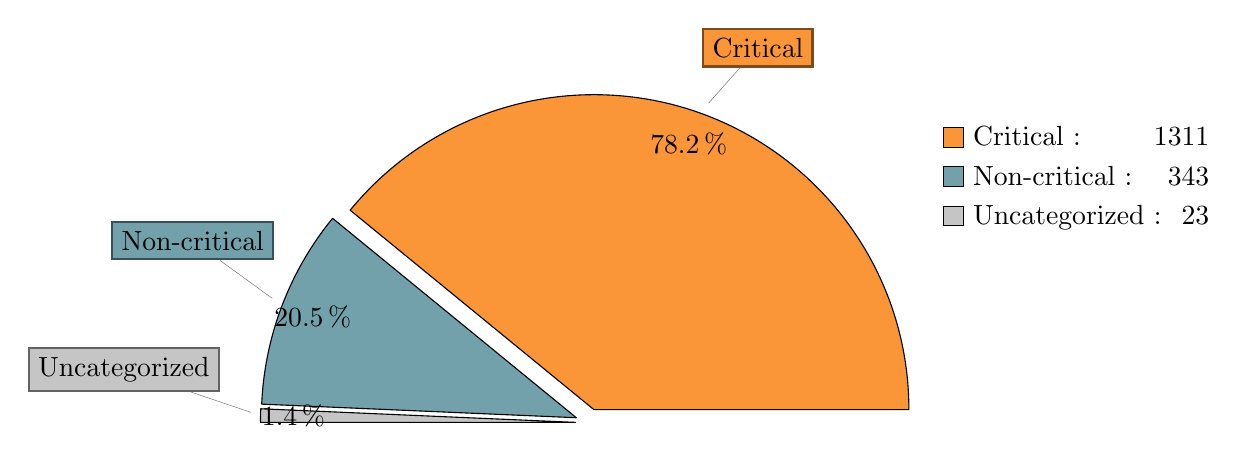
\begin{tikzpicture}
        \path[%
            % style options
            dc sector/.append style={shift={(\MedA:5pt)}}, % shift all sectors
            dc dtag/.append style={},
            dc legend/.append style={text width=3cm, align=right},
            every pin/.style={fill=\Cj,draw=\Cj!50!black,thick},
            % diagram options
            /DiagCirc/.cd,
            value list={1311/Critical,343/Non-critical,23/Uncategorized},
            color list={"color10","color11","color12"},
            angle max=180,             % semi-circular
            angle corr={0,0,0,0,0},    % correct round angle error
            legend=\N\ :\hfill \V,     % custom legend
            factor=.9,
            percent corr={0,0,0,0,0}, % correct round percent error
            shift sector={0,0,0,0,0}, % shift individual sector
            tags=\P,                   % custom sector nodes
            sup loop={% custom features :       
                %--- pin directions just for THIS figure --------------
                %   slice 0   slice 1        slice 2
                \def\Pin{{87,  100,           150}}
                %   ↑   moved Critical up to 80° so it clears the legend
                \pgfmathparse{array(\Pin,\j)}
                \edef\Pinj{\pgfmathresult}
                \node[pin=\Pinj:\N] at (DC\j) {};
                },
            diagram] ;
        \end{tikzpicture}
    }
    \caption{Distribution of categorizations from version diff A}
    \label{fig:categorization_A}
\end{figure}

\begin{figure}[H]
    \centering
    \resizebox{0.92\textwidth}{!}{%
        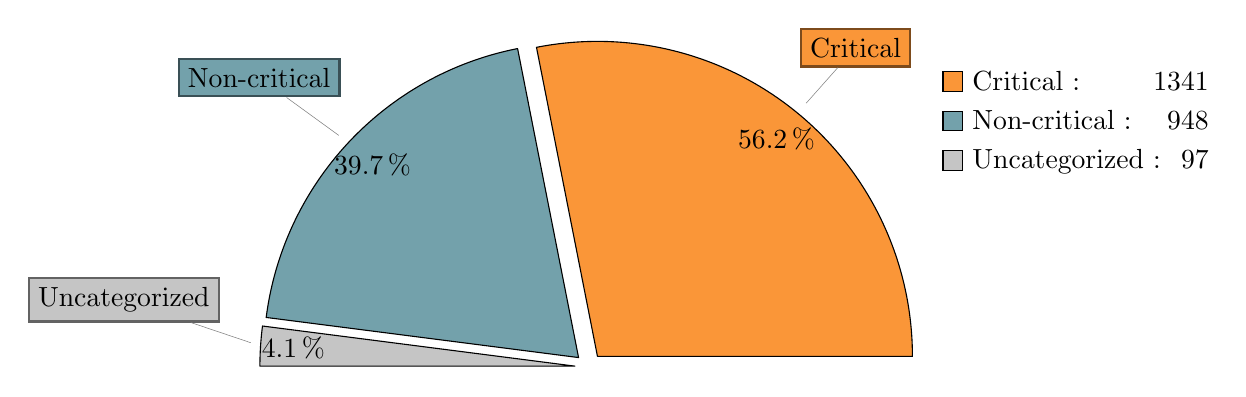
\begin{tikzpicture}
        \path[%
            % style options
            dc sector/.append style={shift={(\MedA:5pt)}}, % shift all sectors
            dc dtag/.append style={},
            dc legend/.append style={text width=3cm, align=right},
            every pin/.style={fill=\Cj,draw=\Cj!50!black,thick},
            % diagram options
            /DiagCirc/.cd,
            value list={1341/Critical,948/Non-critical,97/Uncategorized},
            color list={"color10","color11","color12"},
            angle max=180,             % semi-circular
            angle corr={0,0,0,0,0},    % correct round angle error
            legend=\N\ :\hfill \V,     % custom legend
            factor=.9,
            percent corr={0,0,0,0,0}, % correct round percent error
            shift sector={0,0,0,0,0}, % shift individual sector
            tags=\P,                   % custom sector nodes
            sup loop={% custom features :       
                %--- pin directions just for THIS figure --------------
                %   slice 0   slice 1        slice 2
                \def\Pin{{87,  100,           150}}
                %   ↑   moved Critical up to 80° so it clears the legend
                \pgfmathparse{array(\Pin,\j)}
                \edef\Pinj{\pgfmathresult}
                \node[pin=\Pinj:\N] at (DC\j) {};
                },
            diagram] ;
        
        \end{tikzpicture}
    }
    \caption{Distribution of categorizations from version diff B}
    \label{fig:categorization_B}
\end{figure}

\begin{figure}[H]
    \centering
    \resizebox{0.92\textwidth}{!}{%
        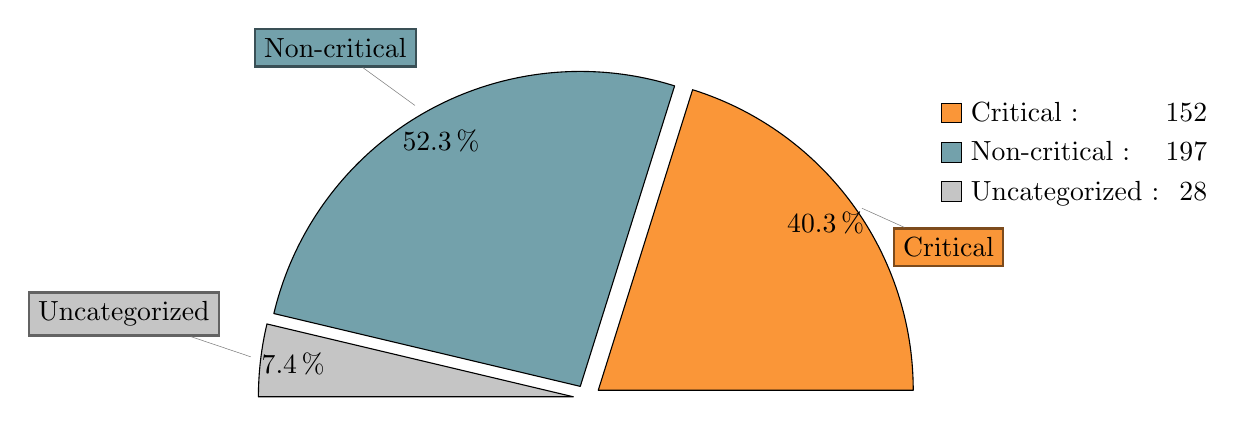
\begin{tikzpicture}
        \path[%
            % style options
            dc sector/.append style={shift={(\MedA:5pt)}}, % shift all sectors
            dc dtag/.append style={},
            dc legend/.append style={text width=3cm, align=right},
            every pin/.style={fill=\Cj,draw=\Cj!50!black,thick},
            % diagram options
            /DiagCirc/.cd,
            value list={152/Critical,197/Non-critical,28/Uncategorized},
            color list={"color10","color11","color12"},
            angle max=180,             % semi-circular
            angle corr={0,0,0,0,0},    % correct round angle error
            legend=\N\ :\hfill \V,     % custom legend
            factor=.9,
            percent corr={0,0,0,0,0}, % correct round percent error
            shift sector={0,0,0,0,0}, % shift individual sector
            tags={%
                \P                   % custom sector nodes
            },
            sup loop={% custom features :       
                %--- pin directions just for THIS figure --------------
                %   slice 0   slice 1        slice 2
                \def\Pin{{330,  100,           150}}
                %   ↑   moved Critical up to 80° so it clears the legend
                \pgfmathparse{array(\Pin,\j)}
                \edef\Pinj{\pgfmathresult}
                \node[pin=\Pinj:\N] at (DC\j) {};
            },
            diagram] ;
        
        \end{tikzpicture}
    }
    \caption{Distribution of categorizations from version diff C}
    \label{fig:categorization_C}
\end{figure}



% critical cat piecharts %
\subsubsection{Critical Categorization Distribution}
The critical changes identified during the pipeline analysis are divided into six predefined categories, previously introduced in Section~\ref{sec:method:changes_to_categorize}. These categories represent specific types of changes that are considered highly impactful, directly affecting the application's functionality, security, or data management. 
A detailed breakdown of the distribution of detected hits for each critical category is presented in Figures~\ref{fig:critical_changes_A}, \ref{fig:critical_changes_B}, and \ref{fig:critical_changes_C}. These figures show the number of times each critical category was assigned to a detected change across the three analyzed version differences (A, B, and C).
It is important to note that the term "hit" does not directly correspond to a unique change. A single detected change can belong to multiple categories, meaning it can generate multiple hits if categorized under several critical categories. This allows for a more comprehensive view of how changes are categorized, capturing the full scope of their impact.


\begin{figure}[H]
    \centering
    \resizebox{0.8\textwidth}{!}{%
        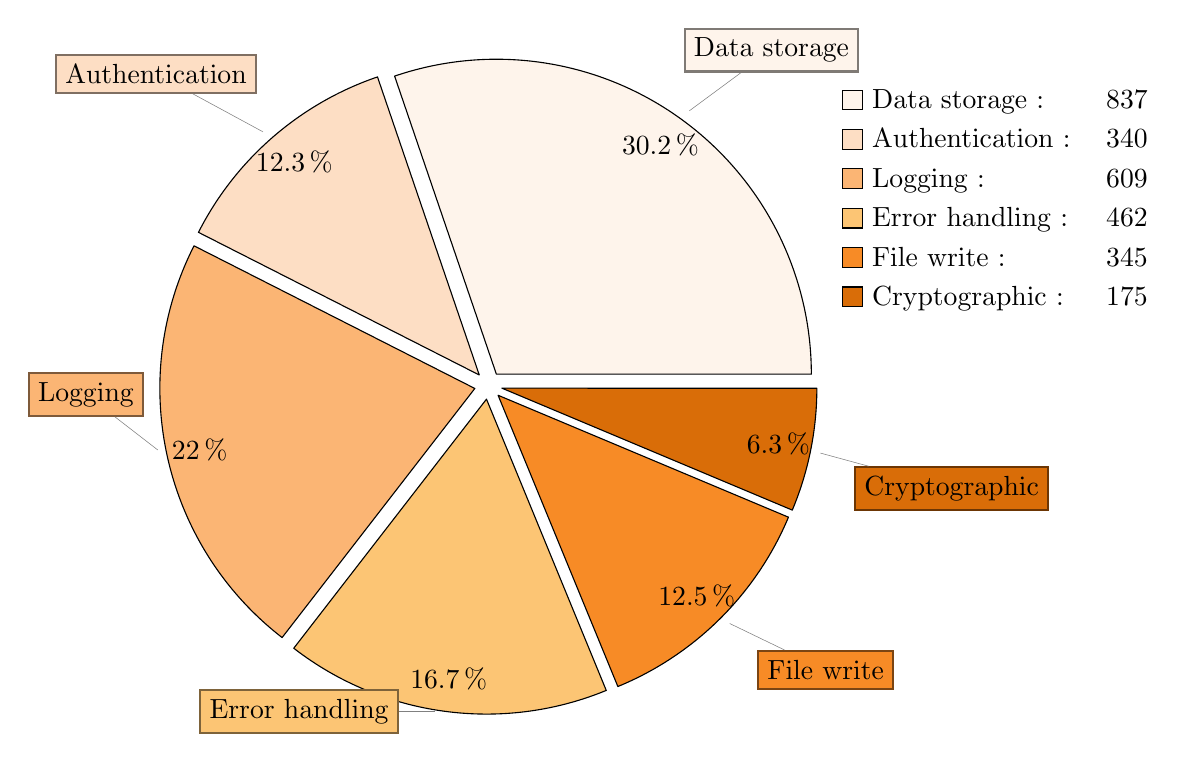
\begin{tikzpicture}
        \path[%
            % style options
            dc sector/.append style={shift={(\MedA:5pt)}}, % shift all sectors
            dc dtag/.append style={},
            dc legend/.append style={text width=3.5cm, align=right},
            every pin/.style={fill=\Cj,draw=\Cj!50!black,thick},
            % diagram options
            /DiagCirc/.cd,
            value list={
                837/Data storage,
                340/Authentication,
                609/Logging,
                462/Error handling,
                345/File write,
                175/Cryptographic
            },
            angle max=360,             % semi-circular
            angle corr={0,0,0,0,0,0},    % correct round angle error
            legend=\N\ :\hfill \V,     % custom legend
            factor=.9,
            percent corr={0,0,0,0,0,0}, % correct round percent error
            shift sector={0,0,0,0,0,0}, % shift individual sector
            tags={%
                \P                   % custom sector nodes
            },
            sup loop={% custom features :       
                %--- pin directions just for THIS figure --------------
                %   slice 0, slice 1, ..., 
                \def\Pin{{85, 110, 120, 180, 320, 340}}
                %   ↑   moved Critical up to 80° so it clears the legend
                \pgfmathparse{array(\Pin,\j)}
                \edef\Pinj{\pgfmathresult}
                \node[pin=\Pinj:\N] at (DC\j) {};
            },
            diagram] ;
        
        \end{tikzpicture}
    }
    \caption{Distribution of hits for each critical category from analysis of version diff A}
    \label{fig:critical_changes_A}
\end{figure}

\begin{figure}[H]
    \centering
    \resizebox{0.8\textwidth}{!}{%
        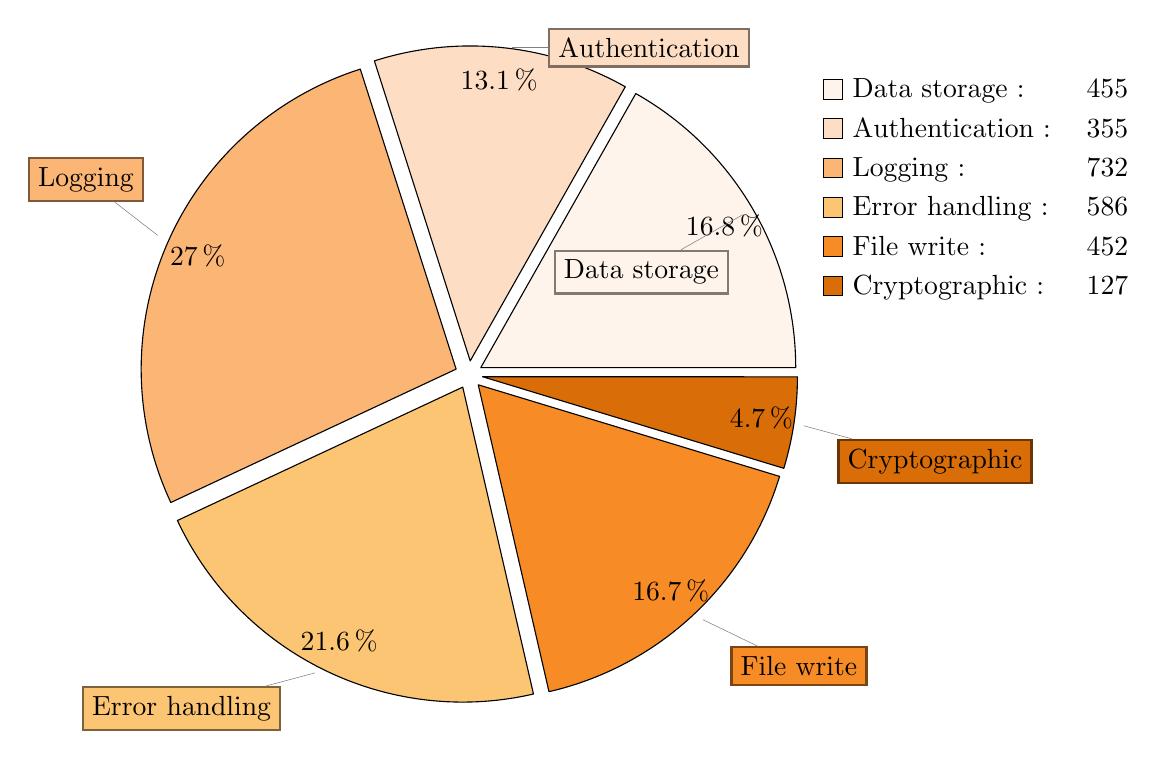
\begin{tikzpicture}
        \path[%
            % style options
            dc sector/.append style={shift={(\MedA:5pt)}}, % shift all sectors
            dc dtag/.append style={},
            dc legend/.append style={text width=3.5cm, align=right},
            every pin/.style={fill=\Cj,draw=\Cj!50!black,thick},
            % diagram options
            /DiagCirc/.cd,
            value list={
                455/Data storage,
                355/Authentication,
                732/Logging,
                586/Error handling,
                452/File write,
                127/Cryptographic
            },
            angle max=360,             % semi-circular
            angle corr={0,0,0,0,0,0},    % correct round angle error
            legend=\N\ :\hfill \V,     % custom legend
            factor=.9,
            percent corr={0,0,0,0,0,0}, % correct round percent error
            shift sector={0,0,0,0,0,0}, % shift individual sector
            tags={%
                \P                   % custom sector nodes
            },
            sup loop={% custom features :       
                %--- pin directions just for THIS figure --------------
                %   slice 0, slice 1, ..., 
                \def\Pin{{240, 0, 120, 200, 320, 340}}
                %   ↑   moved Critical up to 80° so it clears the legend
                \pgfmathparse{array(\Pin,\j)}
                \edef\Pinj{\pgfmathresult}
                \node[pin=\Pinj:\N] at (DC\j) {};
            },
            diagram] ;
        
        \end{tikzpicture}
    }
    \caption{Distribution of hits for each critical category from analysis of version diff B}
    \label{fig:critical_changes_B}
\end{figure}

\begin{figure}[H]
    \centering
    \resizebox{0.8\textwidth}{!}{%
        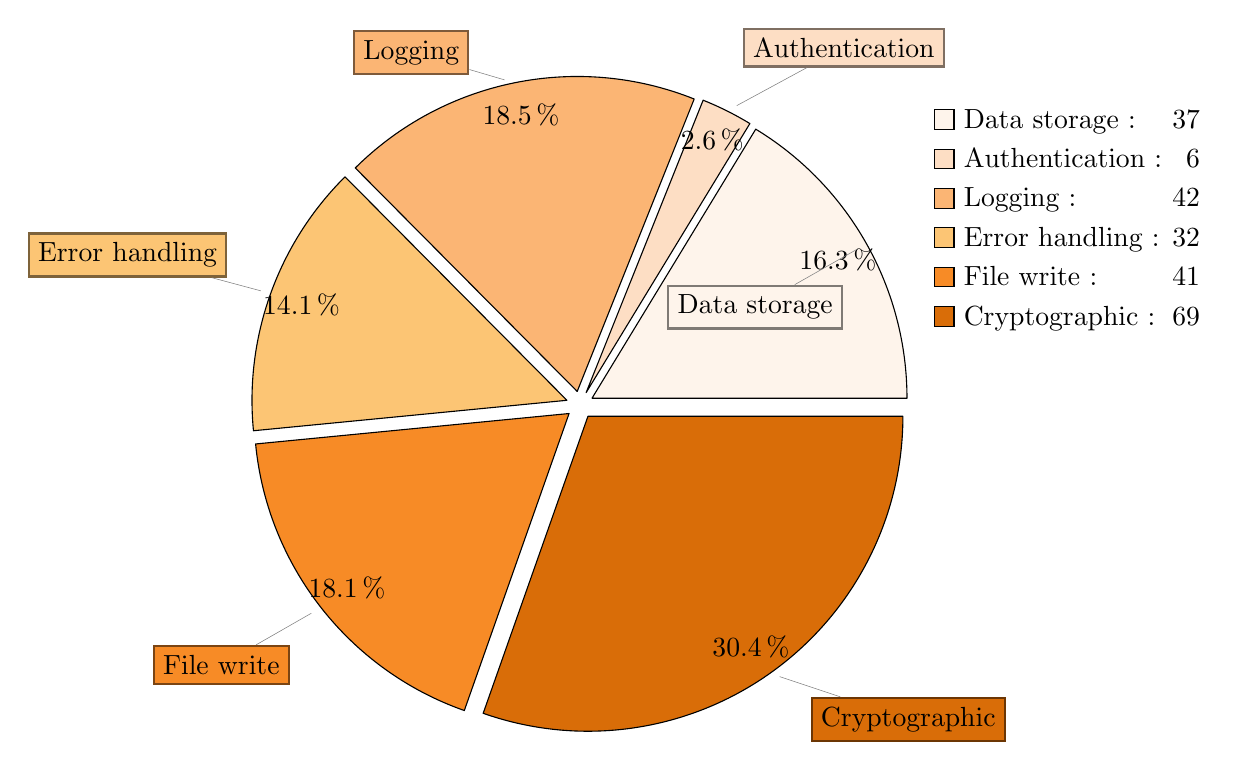
\begin{tikzpicture}
        \path[%
            % style options
            dc sector/.append style={shift={(\MedA:5pt)}}, % shift all sectors
            dc dtag/.append style={},
            dc legend/.append style={text width=3cm, align=right},
            every pin/.style={fill=\Cj,draw=\Cj!50!black,thick},
            % diagram options
            /DiagCirc/.cd,
            value list={
                37/Data storage,
                6/Authentication,
                42/Logging,
                32/Error handling,
                41/File write,
                69/Cryptographic
            },
            angle max=360,             % semi-circular
            angle corr={0,0,0,0,0,0},    % correct round angle error
            legend=\N\ :\hfill \V,     % custom legend
            factor=.9,
            percent corr={0,0,0,0,0,0}, % correct round percent error
            shift sector={0,0,0,0,0,0}, % shift individual sector
            tags={%
                \P                   % custom sector nodes
            },
            sup loop={% custom features :       
                %--- pin directions just for THIS figure --------------
                %   slice 0, slice 1, ..., 
                \def\Pin{{240, 70, 170, 160, 230, 330}}
                %   ↑   moved Critical up to 80° so it clears the legend
                \pgfmathparse{array(\Pin,\j)}
                \edef\Pinj{\pgfmathresult}
                \node[pin=\Pinj:\N] at (DC\j) {};
            },
            diagram] ;
        
        \end{tikzpicture}
    }
    \caption{Distribution of hits for each critical category from analysis of version diff C}
    \label{fig:critical_changes_C}
\end{figure}

An analysis of Figures~\ref{fig:critical_changes_A}, \ref{fig:critical_changes_B}, and \ref{fig:critical_changes_C} reveals that the distribution of critical categories remains relatively consistent across the three version differences, despite substantial variations in the total number of detected changes for each version. This consistency suggests that the types of critical changes detected are generally similar, even though the code modifications and their underlying purposes may differ significantly between versions.

This observation can be interpreted in two contrasting ways. On the one hand, it may be viewed as a potential limitation of the categorization process, as it could imply that the pipeline detects similar categories regardless of the actual nature of the changes. Given that different versions of an application are unlikely to have identical change patterns, this uniform distribution might be seen as a sign of overgeneralization.
On the other hand, this consistency can also be considered a strength of the analysis. It demonstrates that even minor modifications in the source code can lead to distinct execution paths, each captured and categorized by the pipeline. This ability to detect and classify a wide range of changes—regardless of their scale—highlights the sensitivity and thoroughness of the tool.
A more detailed discussion of this observation, including its implications and potential improvements, is provided in Section~\ref{sec:discussion-results}.








% noncritical cat dist %
\subsubsection{Non-critical categorization distribution}
The non-critical changes identified during the pipeline analysis are categorized into four distinct categories, as previously introduced in Section~\ref{sec:method:changes_to_categorize}. These categories capture modifications that, while relevant, do not directly impact the core functionality, security, or data handling of the application. Such changes typically include user interface updates, logging adjustments, and other non-essential modifications.
A detailed breakdown of the distribution of hits within each non-critical category is presented in Figures~\ref{fig:noncritical_changes_A}, \ref{fig:noncritical_changes_B}, and \ref{fig:noncritical_changes_C}. These figures illustrate how frequently each non-critical category was assigned across the three versions (A, B, and C), providing a clear view of how such changes are distributed in each analyzed version.
It is important to clarify that the term "hit" in this context does not directly correspond to a unique change. A single detected change may be assigned to multiple categories, resulting in multiple hits. For instance, a change that affects both user interface elements and logging functionality would be counted as a hit in both categories. This approach allows for a more comprehensive understanding of the nature of the detected changes.


\begin{figure}[H]
    \centering
    \resizebox{0.92\textwidth}{!}{%
        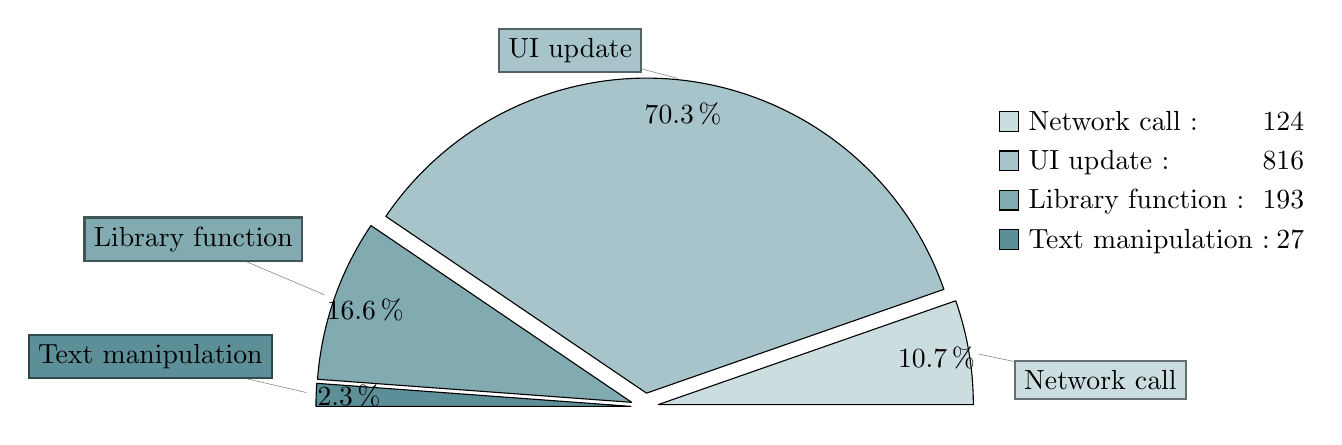
\begin{tikzpicture}
        \path[%
            % style options
            dc sector/.append style={shift={(\MedA:5pt)}}, % shift all sectors
            dc dtag/.append style={},
            dc legend/.append style={text width=3.5cm, align=right},
            every pin/.style={fill=\Cj,draw=\Cj!50!black,thick},
            % diagram options
            /DiagCirc/.cd,
            value list={
                124/Network call,
                816/UI update,
                193/Library function,
                27/Text manipulation
            },
            color list={"color6","color7","color8","color9"},
            angle max=180,             % semi-circular
            angle corr={0,0,0,0,0,0},    % correct round angle error
            legend=\N\ :\hfill \V,     % custom legend
            factor=.9,
            percent corr={0,0,0,0,0,0}, % correct round percent error
            shift sector={0,0,0,0,0,0}, % shift individual sector
            tags={%
                \P                   % custom sector nodes
            },
            sup loop={% custom features :       
                %--- pin directions just for THIS figure --------------
                %   slice 0, slice 1, ..., 
                \def\Pin{{350, 170, 130, 160}}
                %   ↑   moved Critical up to 80° so it clears the legend
                \pgfmathparse{array(\Pin,\j)}
                \edef\Pinj{\pgfmathresult}
                \node[pin=\Pinj:\N] at (DC\j) {};
            },
            diagram] ;
        
        \end{tikzpicture}
    }
    \caption{Distribution of hits for each non-critical category from analysis of version diff A}
    \label{fig:noncritical_changes_A}
\end{figure}

\begin{figure}[H]
    \centering
    \resizebox{0.92\textwidth}{!}{%
        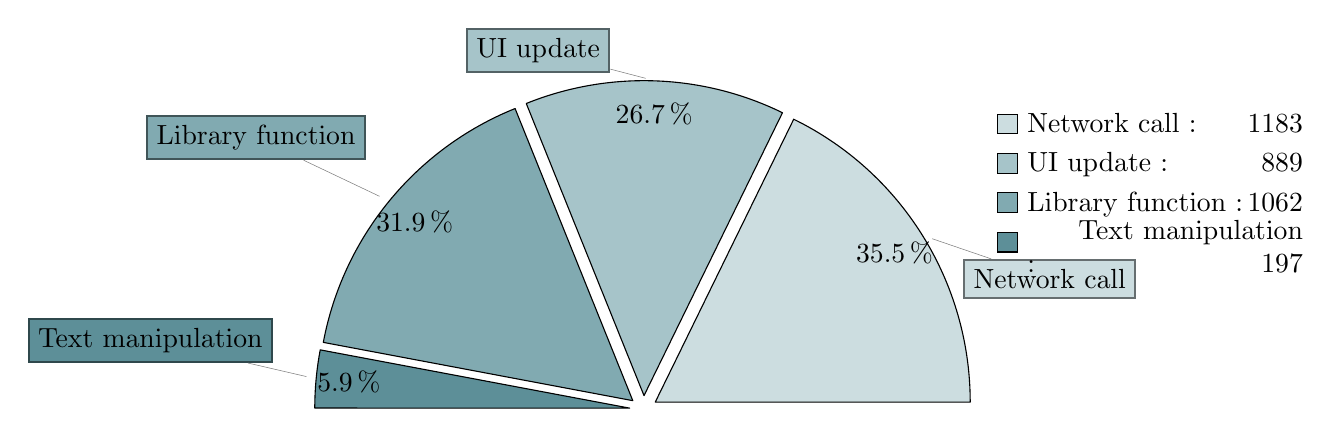
\begin{tikzpicture}
        \path[%
            % style options
            dc sector/.append style={shift={(\MedA:5pt)}}, % shift all sectors
            dc dtag/.append style={},
            dc legend/.append style={text width=3.5cm, align=right},
            every pin/.style={fill=\Cj,draw=\Cj!50!black,thick},
            % diagram options
            /DiagCirc/.cd,
            value list={
                1183/Network call,
                889/UI update,
                1062/Library function,
                197/Text manipulation
            },
            color list={"color6","color7","color8","color9"},
            angle max=180,             % semi-circular
            angle corr={0,0,0,0,0,0},    % correct round angle error
            legend=\N\ :\hfill \V,     % custom legend
            factor=.9,
            percent corr={0,0,0,0,0,0}, % correct round percent error
            shift sector={0,0,0,0,0,0}, % shift individual sector
            tags={%
                \P                   % custom sector nodes
            },
            sup loop={% custom features :       
                %--- pin directions just for THIS figure --------------
                %   slice 0, slice 1, ..., 
                \def\Pin{{330, 170, 120, 160}}
                %   ↑   moved Critical up to 80° so it clears the legend
                \pgfmathparse{array(\Pin,\j)}
                \edef\Pinj{\pgfmathresult}
                \node[pin=\Pinj:\N] at (DC\j) {};
            },
            diagram] ;
        
        \end{tikzpicture}
    }
    \caption{Distribution of hits for each non-critical category from analysis of version diff B}
    \label{fig:noncritical_changes_B}
\end{figure}

\begin{figure}[H]
    \centering
    \resizebox{0.92\textwidth}{!}{%
        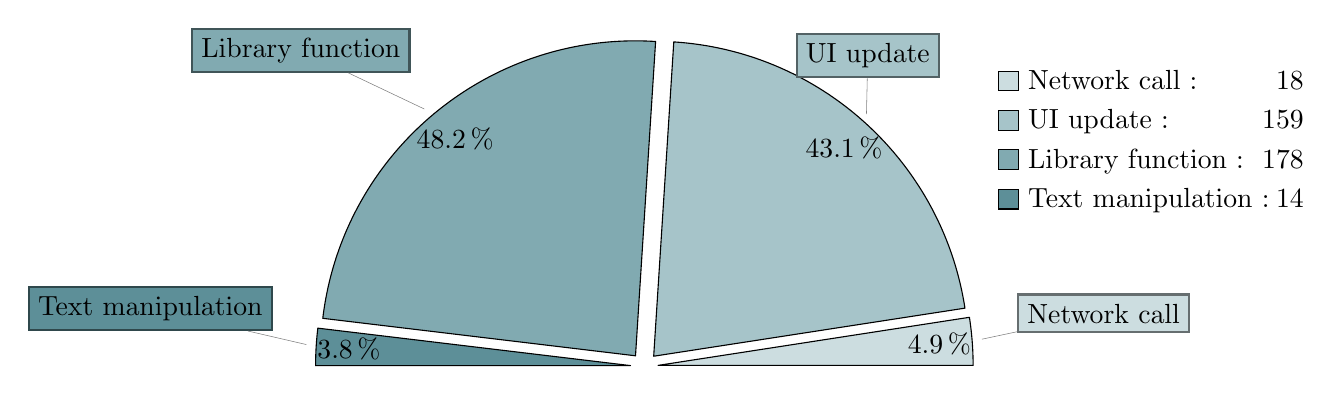
\begin{tikzpicture}
        \path[%
            % style options
            dc sector/.append style={shift={(\MedA:5pt)}}, % shift all sectors
            dc dtag/.append style={},
            dc legend/.append style={text width=3.5cm, align=right},
            every pin/.style={fill=\Cj,draw=\Cj!50!black,thick},
            % diagram options
            /DiagCirc/.cd,
            value list={
                18/Network call,
                159/UI update,
                178/Library function,
                14/Text manipulation
            },
            color list={"color6","color7","color8","color9"},
            angle max=180,             % semi-circular
            angle corr={0,0,0,0,0,0},    % correct round angle error
            legend=\N\ :\hfill \V,     % custom legend
            factor=.9,
            percent corr={0,0,0,0,0,0}, % correct round percent error
            shift sector={0,0,0,0,0,0}, % shift individual sector
            tags={%
                \P                   % custom sector nodes
            },
            sup loop={% custom features :       
                %--- pin directions just for THIS figure --------------
                %   slice 0, slice 1, ..., 
                \def\Pin{{10, 88, 120, 160}}
                %   ↑   moved Critical up to 80° so it clears the legend
                \pgfmathparse{array(\Pin,\j)}
                \edef\Pinj{\pgfmathresult}
                \node[pin=\Pinj:\N] at (DC\j) {};
            },
            diagram] ;
        
        \end{tikzpicture}
    }
    \caption{Distribution of hits for each non-critical category from analysis of version diff C}
    \label{fig:noncritical_changes_C}
\end{figure}

The data presented in Figures~\ref{fig:noncritical_changes_A}, \ref{fig:noncritical_changes_B}, and \ref{fig:noncritical_changes_C} reveal a clear pattern: the categories \codebox{UI update} and \codebox{Library function} are the most frequently detected among non-critical changes. This outcome is consistent with the nature of the Signal Android application, which serves as the test subject for this analysis. Given that Signal is a messaging app with a user interface that undergoes frequent updates, it is unsurprising that UI-related changes are detected most often. 

Similarly, the high frequency of the \codebox{Library function} category can be attributed to Signal’s reliance on numerous external libraries. Any upstream updates or modifications within these libraries are automatically registered as changes during the analysis. This means that even if the Signal application code itself remains unchanged, updates in the external libraries it depends on are still captured by the pipeline.

\subsubsection{Categories Resulting in \textit{Correct} vs \textit{Incorrect} Categorization}
\label{sec:result:categorization_distributions:categories_resulting_in_correct_incorrect_categorizations}

This section examines the accuracy of the pipeline’s categorization by comparing the number of hits per category that were classified \textit{correctly} versus those that were \textit{incorrectly} categorized. The results are visualized in bar charts in Figures~\ref{fig:category_comparison_A}, \ref{fig:category_comparison_B}, and \ref{fig:category_comparison_C}. 

Each bar chart displays the number of hits (instances) in each category, separated into two groups: correctly categorized and incorrectly categorized. A correct categorization means that the categories assigned by the pipeline match those determined through the manual analysis. An incorrect categorization occurs when the pipeline assigns categories that do not match the manually identified ones. This comparison provides insights into the pipeline’s classification performance for each category.

%, where the Y-axis is the number of assignments, and the X-axis is the category.

\begin{figure}[H]
    \centering
    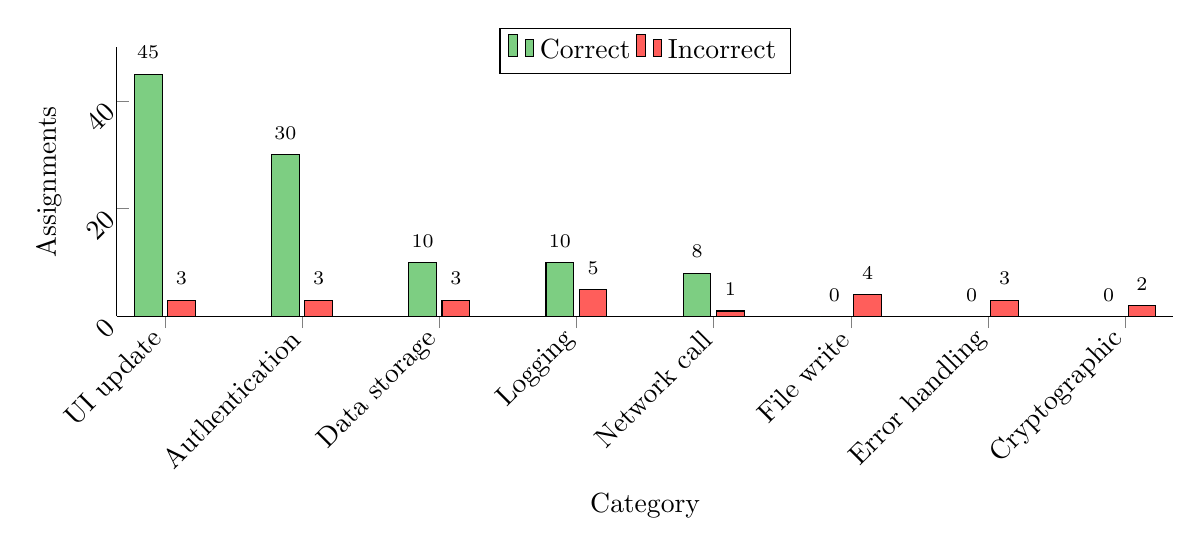
\begin{tikzpicture}
      \begin{axis}[
        width=15cm,
        height=5.0cm,
        ybar,
        bar width=10pt,
        symbolic x coords={\codebox{UI update},\codebox{Authentication},\codebox{Data storage},\codebox{Logging},\codebox{Network call},\codebox{File write},\codebox{Error handling},\codebox{Cryptographic}},
        xtick=data,
        tick label style={font=\normalsize,rotate=45,anchor=east},
        enlarge x limits=0.05,
        xlabel={Category},
        ylabel={Assignments},
        ymin=0, ymax=50,
        nodes near coords,
        every node near coord/.append style={font=\scriptsize,yshift=2pt},
        axis x line*=bottom,
        axis y line*=left,
        legend style={at={(0.5,0.9)},anchor=south,legend columns=-1},
        legend cell align={left}
      ]
        % ─── Correct (green) ──────────────────────────────
        \addplot[ybar,fill=correct_color] coordinates {
          (\codebox{UI update},45) (\codebox{Authentication},30) (\codebox{Data storage},10) (\codebox{Logging},10) (\codebox{Network call},8)
          (\codebox{File write},0) (\codebox{Error handling},0) (\codebox{Cryptographic},0)
        };
        % ─── Incorrect (red) ─────────────────────────────
        \addplot[ybar,fill=incorrect_color] coordinates {
          (\codebox{UI update},3) (\codebox{Authentication},3) (\codebox{Data storage},3) (\codebox{Logging},5) (\codebox{Network call},1)
          (\codebox{File write},4) (\codebox{Error handling},3) (\codebox{Cryptographic},2)
        };
        \legend{Correct,Incorrect}
      \end{axis}
    \end{tikzpicture}
    \caption{Amount of correctly vs incorrectly assigned categories, per category, for version diff A}
    \label{fig:category_comparison_A}
\end{figure}

\begin{figure}[H]
    \centering
    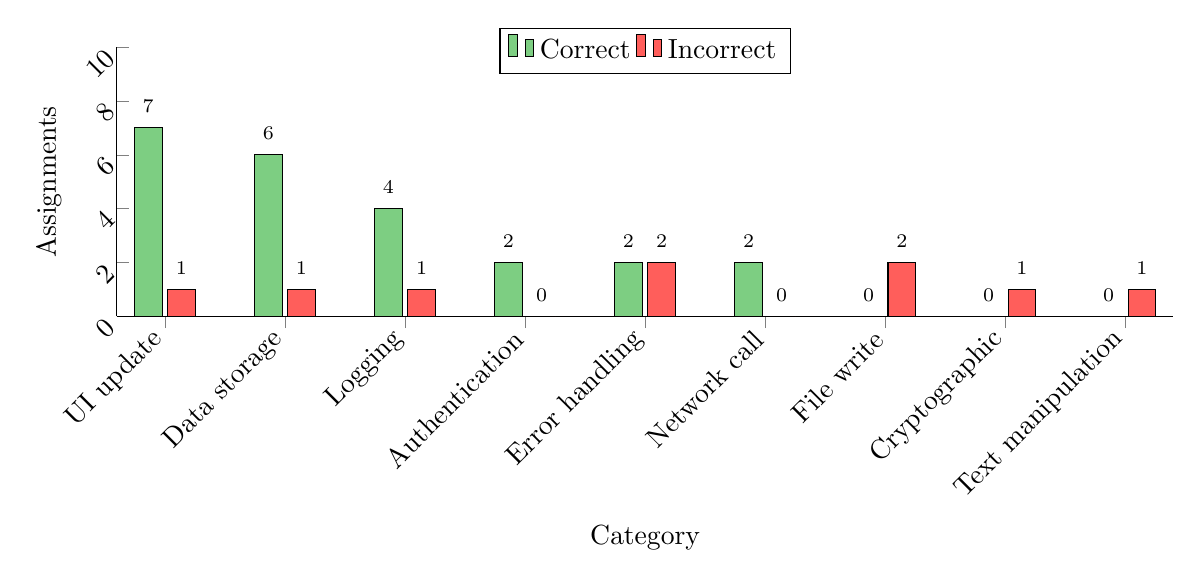
\begin{tikzpicture}
      \begin{axis}[
        width=15cm,
        height=5.0cm,
        ybar,
        bar width=10pt,
        symbolic x coords={\codebox{UI update},\codebox{Data storage},\codebox{Logging},\codebox{Authentication},\codebox{Error handling},\codebox{Network call},\codebox{File write},\codebox{Cryptographic},\codebox{Text manipulation}},
        xtick=data,
        tick label style={font=\normalsize,rotate=45,anchor=east},
        enlarge x limits=0.05,
        xlabel={Category},
        ylabel={Assignments},
        ymin=0, ymax=10,
        nodes near coords,
        every node near coord/.append style={font=\scriptsize,yshift=2pt},
        axis x line*=bottom,
        axis y line*=left,
        legend style={at={(0.5,0.9)},anchor=south,legend columns=-1},
        legend cell align={left}
      ]
        % ─── Correct (green) ──────────────────────────────
        \addplot[ybar,fill=correct_color] coordinates {
          (\codebox{UI update},7) (\codebox{Data storage},6) (\codebox{Logging},4) (\codebox{Authentication},2) (\codebox{Error handling},2) (\codebox{Network call},2)
          (\codebox{File write},0) (\codebox{Cryptographic},0) (\codebox{Text manipulation},0)
        };
        % ─── Incorrect (red) ─────────────────────────────
        \addplot[ybar,fill=incorrect_color] coordinates {
          (\codebox{UI update},1) (\codebox{Data storage},1) (\codebox{Logging},1) (\codebox{Authentication},0) (\codebox{Error handling},2) (\codebox{Network call},0)
          (\codebox{File write},2) (\codebox{Cryptographic},1) (\codebox{Text manipulation},1)
        };
        \legend{Correct,Incorrect}
      \end{axis}
    \end{tikzpicture}
    \caption{Amount of correctly vs incorrectly assigned categories, per category, for version diff B}
    \label{fig:category_comparison_B}
\end{figure}

\begin{figure}[H]
    \centering
    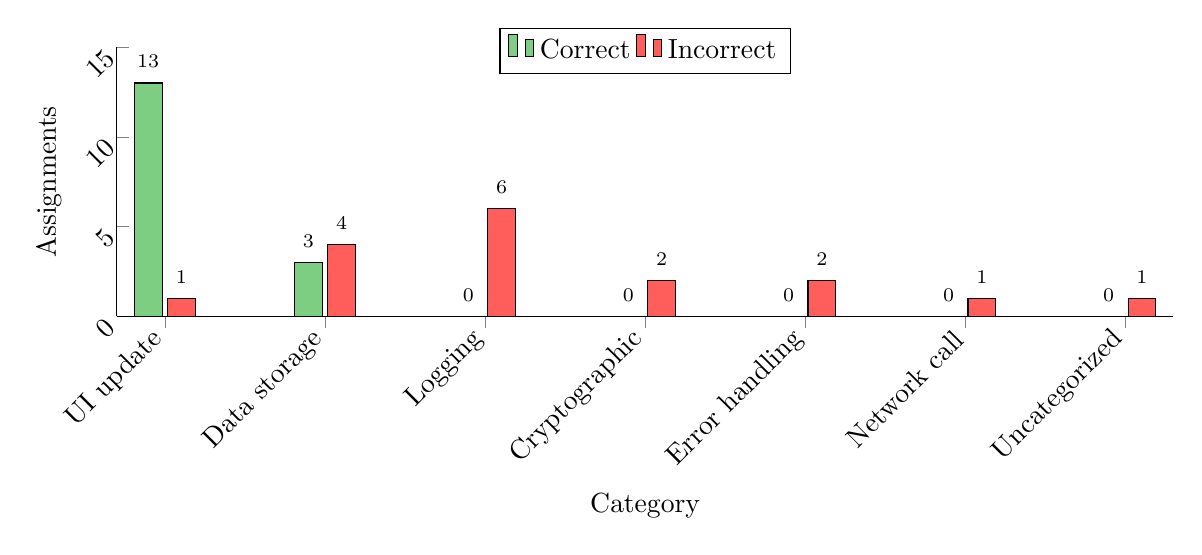
\begin{tikzpicture}
      \begin{axis}[
        width=15cm,
        height=5.0cm,
        ybar,
        bar width=10pt,
        symbolic x coords={\codebox{UI update},\codebox{Data storage},\codebox{Logging},\codebox{Cryptographic},\codebox{Error handling},\codebox{Network call},\codebox{Uncategorized}},
        xtick=data,
        tick label style={font=\normalsize,rotate=45,anchor=east},
        enlarge x limits=0.05,
        xlabel={Category},
        ylabel={Assignments},
        ymin=0, ymax=15,
        nodes near coords,
        every node near coord/.append style={font=\scriptsize,yshift=2pt},
        axis x line*=bottom,
        axis y line*=left,
        legend style={at={(0.5,0.9)},anchor=south,legend columns=-1},
        legend cell align={left}
      ]
        % ─── Correct (green) ──────────────────────────────
        \addplot[ybar,fill=correct_color] coordinates {
          (\codebox{UI update},13) (\codebox{Data storage},3) (\codebox{Logging},0) (\codebox{Cryptographic},0)
          (\codebox{Error handling},0) (\codebox{Network call},0) (\codebox{Uncategorized},0)
        };
        % ─── Incorrect (red) ─────────────────────────────
        \addplot[ybar,fill=incorrect_color] coordinates {
          (\codebox{UI update},1) (\codebox{Data storage},4) (\codebox{Logging},6) (\codebox{Cryptographic},2)
          (\codebox{Error handling},2) (\codebox{Network call},1) (\codebox{Uncategorized},1)
        };
        \legend{Correct,Incorrect}
      \end{axis}
    \end{tikzpicture}
    \caption{Amount of correctly vs incorrectly assigned categories, per category, for version diff C}
    \label{fig:category_comparison_C}
\end{figure}

From Figures~\ref{fig:category_comparison_A}, \ref{fig:category_comparison_B}, and \ref{fig:category_comparison_C}, it is evident that the category \codebox{UI update} is the most frequently assigned category across all version differences, with a total of 65 assignments. This category shows a substantial lead over the next two most frequently assigned categories: \codebox{Authentication}, which has 32 assignments, and \codebox{Data storage}, which has 19 assignments. 

These three categories—\codebox{UI update}, \codebox{Authentication}, and \codebox{Data storage}—also exhibit the highest correct-to-incorrect ratio, indicating that they are not only frequently assigned but also accurately classified by the pipeline. A more detailed discussion of this performance, including the correct-to-incorrect ratio for each category, is provided later in this chapter in Section~\ref{sec:res:comprehensive_summary}.

\subsection{Keyword Distributions}

This section presents an analysis of the distribution of keywords detected during the pipeline analysis, focusing on their effectiveness in triggering critical or non-critical categories. The results include the total number of hits for each keyword, indicating how often each keyword led to a categorization decision. These hits are further divided into two groups: \textit{correct} and \textit{incorrect}, providing insights into the accuracy of keyword-based classification.

\subsubsection{Keywords Resulting in Critical and Non-Critical Categorizations}

The total number of hits for each keyword that triggered a critical or non-critical classification during the regular-expression analysis is displayed in Figures \ref{fig:commonly_used_words_A}, \ref{fig:commonly_used_words_B}, and \ref{fig:commonly_used_words_C}. Each figure visualizes how frequently each keyword was detected, along with a breakdown of how many of these detections led to correct or incorrect categorizations. This analysis helps identify which keywords are most effective at correctly classifying changes and which may require further refinement to improve accuracy.


\begin{figure}[H]
    \centering
    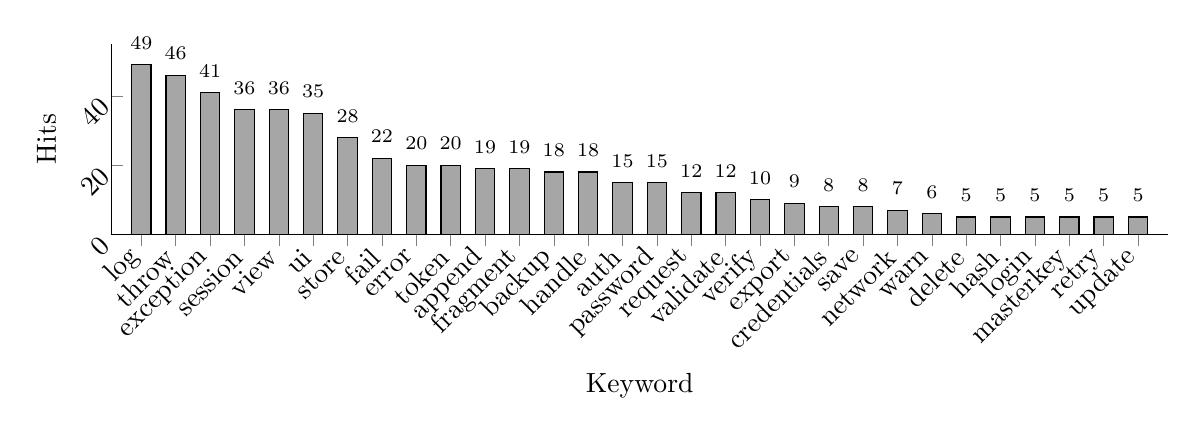
\begin{tikzpicture}
      \begin{axis}[
        width=15cm,
        height=4.0cm,
        ybar,
        bar width=7pt,
        symbolic x coords={
            log,throw,exception,session,view,ui,store,fail,error,token,
            append,fragment,backup,handle,auth,password,request,validate,
            verify,export,credentials,save,network,warn,delete,hash,login,
            masterkey,retry,update},
        xtick=data,
        tick label style={font=\normalsize,rotate=45,anchor=east},
        enlarge x limits=0.03,
        xlabel={Keyword},
        ylabel={Hits},
        ymin=0, ymax=55,
        nodes near coords,
        every node near coord/.append style={font=\scriptsize,yshift=2pt},
        axis x line*=bottom,
        axis y line*=left
      ]
        \addplot[ybar,fill=gray!70] coordinates {
          (log,49) (throw,46) (exception,41) (session,36) (view,36)
          (ui,35) (store,28) (fail,22) (error,20) (token,20) (append,19)
          (fragment,19) (backup,18) (handle,18) (auth,15) (password,15)
          (request,12) (validate,12) (verify,10) (export,9) (credentials,8)
          (save,8) (network,7) (warn,6) (delete,5) (hash,5) (login,5)
          (masterkey,5) (retry,5) (update,5)
        };
      \end{axis}
    \end{tikzpicture}
    \caption{Keyword hits generating categorizations in version diff A. Hits below 5 have been neglected. See Figure \ref{fig:commonly_used_words_A_full} for complete data.}
    \label{fig:commonly_used_words_A}
\end{figure}


\begin{figure}[H]
    \centering
    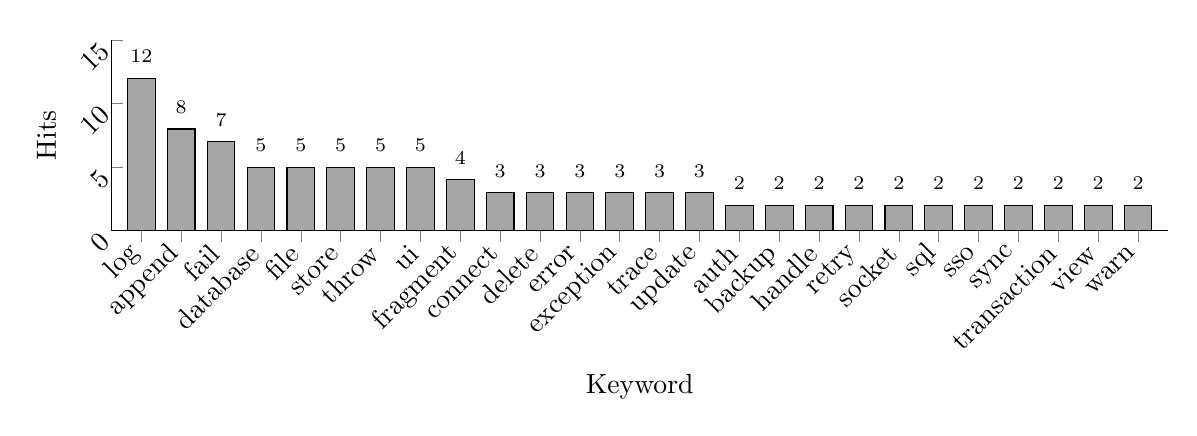
\begin{tikzpicture}
      \begin{axis}[
        width=15cm,
        height=4.0cm,
        ybar,
        bar width=10pt,
        symbolic x coords={
            log,append,fail,database,file,store,throw,ui,fragment,connect,
            delete,error,exception,trace,update,auth,backup,handle,retry,
            socket,sql,sso,sync,transaction,view,warn,commit,credentials,
            debug,decrypt,digest,fetch,hash,refresh,request,send,show,text,
            write},
        xtick=data,
        tick label style={font=\normalsize,rotate=45,anchor=east},
        enlarge x limits=0.03,
        xlabel={Keyword},
        ylabel={Hits},
        ymin=0, ymax=15,
        nodes near coords,
        every node near coord/.append style={font=\scriptsize,yshift=2pt},
        axis x line*=bottom,
        axis y line*=left
      ]
        \addplot[ybar,fill=gray!70] coordinates {
          (log,12) (append,8) (fail,7) (database,5) (file,5) (store,5)
          (throw,5) (ui,5) (fragment,4) (connect,3) (delete,3) (error,3)
          (exception,3) (trace,3) (update,3) (auth,2) (backup,2) (handle,2)
          (retry,2) (socket,2) (sql,2) (sso,2) (sync,2) (transaction,2)
          (view,2) (warn,2)
        };
      \end{axis}
    \end{tikzpicture}
    \caption{Keyword hits generating categorizations in version diff B. Hits below 2 have been neglected. See Figure \ref{fig:commonly_used_words_B_full} for complete data.}
    \label{fig:commonly_used_words_B}
\end{figure}

\begin{figure}[H]
    \centering
    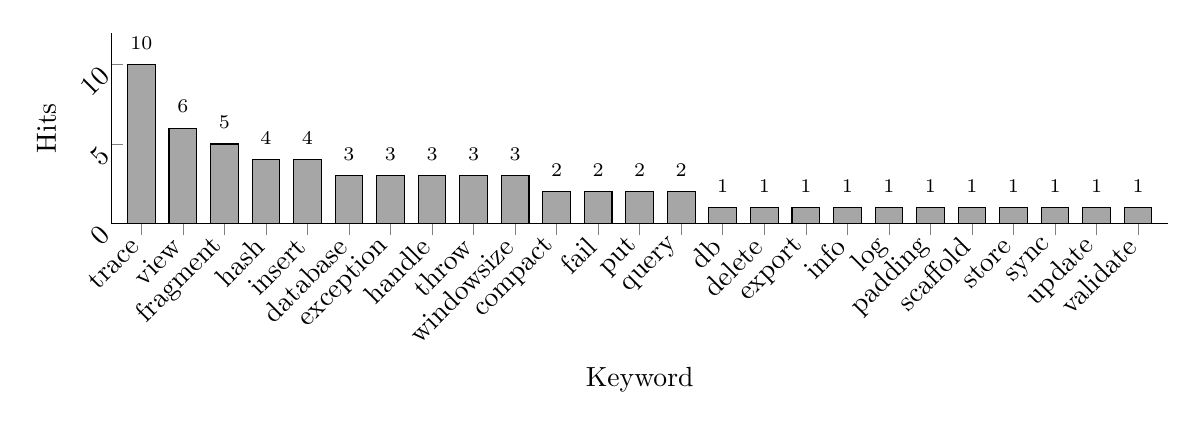
\begin{tikzpicture}
      \begin{axis}[
        width=15cm,
        height=4.0cm,
        ybar,
        bar width=10pt,
        symbolic x coords={
            trace,view,fragment,hash,insert,database,exception,handle,throw,
            windowsize,compact,fail,put,query,db,delete,export,info,log,
            padding,scaffold,store,sync,update,validate},
        xtick=data,
        tick label style={font=\normalsize,rotate=45,anchor=east},
        enlarge x limits=0.03,
        xlabel={Keyword},
        ylabel={Hits},
        ymin=0, ymax=12,
        nodes near coords,
        every node near coord/.append style={font=\scriptsize,yshift=2pt},
        axis x line*=bottom,
        axis y line*=left
      ]
        \addplot[ybar,fill=gray!70] coordinates {
          (trace,10) (view,6) (fragment,5) (hash,4) (insert,4)
          (database,3) (exception,3) (handle,3) (throw,3) (windowsize,3)
          (compact,2) (fail,2) (put,2) (query,2) (db,1) (delete,1)
          (export,1) (info,1) (log,1) (padding,1) (scaffold,1) (store,1)
          (sync,1) (update,1) (validate,1)
        };
      \end{axis}
    \end{tikzpicture}
    \caption{Keyword hits generating categorizations in version diff C (complete)}
    \label{fig:commonly_used_words_C}
\end{figure}



%%%% Commonly used words when incorrect categorization %%%%
\subsubsection{Keywords Resulting in \textit{Incorrect} Categorizations}

This section focuses on the analysis of keywords that resulted in \textit{incorrect} categorizations during the pipeline analysis. Specifically, it examines the total number of times each keyword led to an incorrect classification, providing insights into which keywords are most prone to misclassification.

The results are visualized as bar charts in Figures~\ref{fig:keyword_incorrect_trigger_A}, \ref{fig:keyword_incorrect_trigger_B}, and \ref{fig:keyword_incorrect_trigger_C}. Only keywords that resulted in at least one incorrect categorization are included in these charts. Keywords that did not produce any incorrect hits are excluded to maintain clarity and focus on problematic keywords. This analysis is essential for identifying which keywords may require further refinement or adjustment in the pipeline’s categorization logic to improve overall classification accuracy.


\begin{figure}[H]
    \centering
    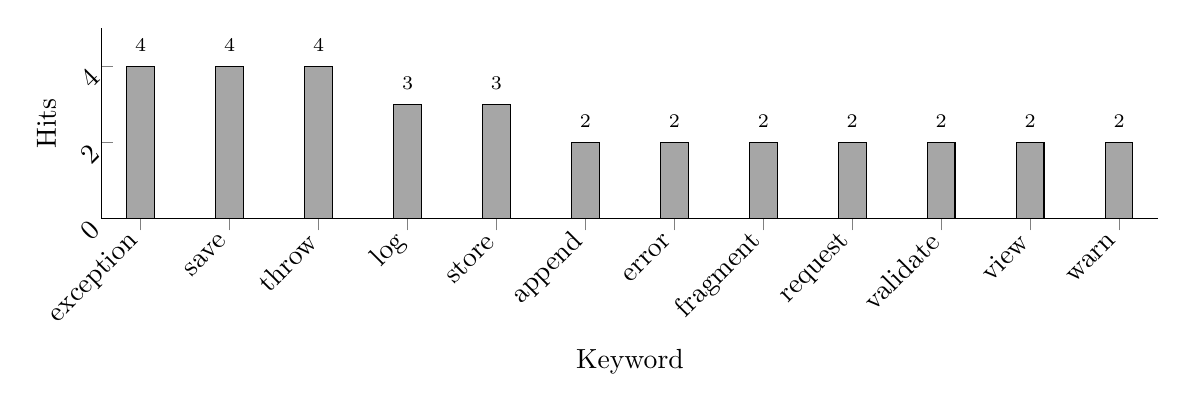
\begin{tikzpicture}
      \begin{axis}[
        width=15cm,
        height=4.0cm,
        ybar,
        bar width=10pt,
        % categorical x-axis
        symbolic x coords={
          exception,save,throw,log,store,append,error,fragment,request,validate,
          view,warn},
        xtick=data,
        tick label style={font=\normalsize,rotate=45,anchor=east},
        enlarge x limits=0.04,
        xlabel={Keyword},
        ylabel={Hits},
        ymin=0, ymax=5,
        nodes near coords,
        every node near coord/.append style={font=\scriptsize,yshift=2pt},
        axis x line*=bottom,
        axis y line*=left
      ]
        \addplot[ybar,fill=gray!70] coordinates {
          (exception,4) (save,4) (throw,4)
          (log,3) (store,3)
          (append,2) (error,2) (fragment,2) (request,2) (validate,2)
          (view,2) (warn,2)
        };
      \end{axis}
    \end{tikzpicture}
    \caption{Keywords resulting in incorrect categorization for version diff A. Hits below 2 have been neglected. See Figure \ref{fig:keyword_incorrect_trigger_A_full} for complete data}
    \label{fig:keyword_incorrect_trigger_A}
\end{figure}

\begin{figure}[H]
    \centering
    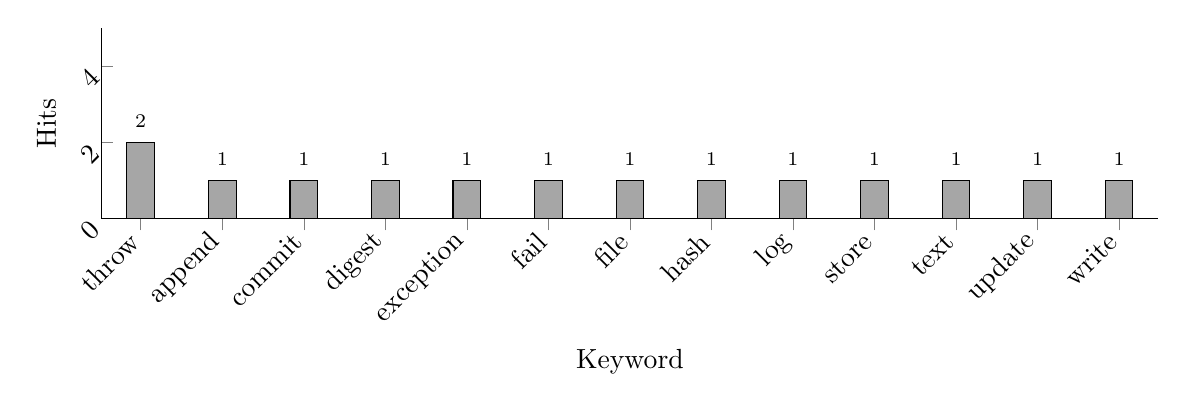
\begin{tikzpicture}
      \begin{axis}[
        width=15cm,
        height=4.0cm,
        ybar,
        bar width=10pt,
        % categorical x-axis
        symbolic x coords={
          throw,append,commit,digest,exception,fail,file,hash,log,store,text,update,write},
        xtick=data,
        tick label style={font=\normalsize,rotate=45,anchor=east},
        enlarge x limits=0.04,
        xlabel={Keyword},
        ylabel={Hits},
        ymin=0, ymax=5,
        nodes near coords,
        every node near coord/.append style={font=\scriptsize,yshift=2pt},
        axis x line*=bottom,
        axis y line*=left
      ]
        \addplot[ybar,fill=gray!70] coordinates {
          (throw,2)
          (append,1) (commit,1) (digest,1) (exception,1) (fail,1)
          (file,1) (hash,1) (log,1) (store,1) (text,1) (update,1) (write,1)
        };
      \end{axis}
    \end{tikzpicture}
    \caption{Keywords resulting in incorrect categorization for version diff B}
    \label{fig:keyword_incorrect_trigger_B}
\end{figure}


\begin{figure}[H]
    \centering
    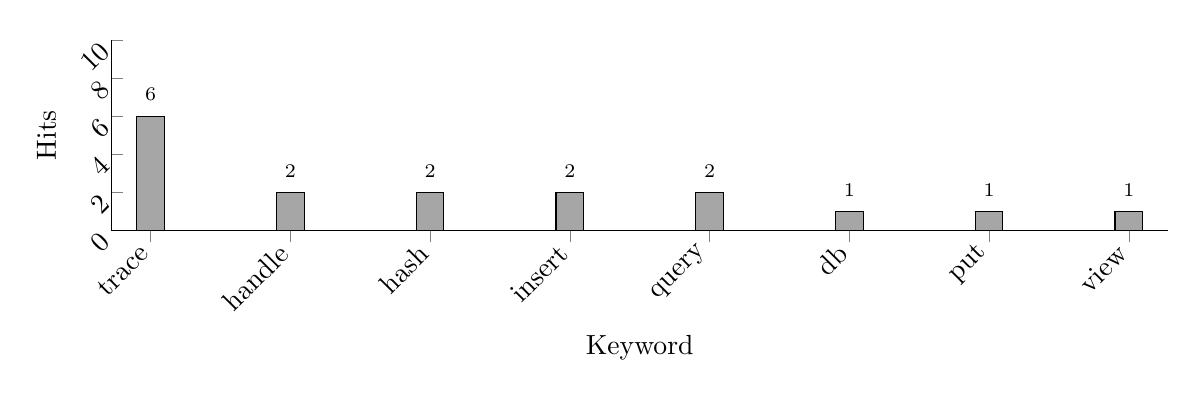
\begin{tikzpicture}
      \begin{axis}[
        width=15cm,
        height=4.0cm,
        ybar,
        bar width=10pt,
        % categorical x-axis
        symbolic x coords={
          trace,handle,hash,insert,query,db,put,view},
        xtick=data,
        tick label style={font=\normalsize,rotate=45,anchor=east},
        enlarge x limits=0.04,
        xlabel={Keyword},
        ylabel={Hits},
        ymin=0, ymax=10,
        nodes near coords,
        every node near coord/.append style={font=\scriptsize,yshift=2pt},
        axis x line*=bottom,
        axis y line*=left
      ]
        \addplot[ybar,fill=gray!70] coordinates {
          (trace,6) (handle,2) (hash,2) (insert,2) (query,2)
          (db,1) (put,1) (view,1)
        };
      \end{axis}
    \end{tikzpicture}
    \caption{Keywords resulting in incorrect categorization for version diff C}
    \label{fig:keyword_incorrect_trigger_C}
\end{figure}




\subsubsection{Accuracy of Keyword Matches}
\label{sec:result:keyword_distribution:Accuracy_of_keyword_matches}

This section examines the accuracy of keyword-based categorizations in the pipeline analysis, focusing on how effectively each keyword triggers correct classifications. The accuracy of keyword matches is visualized in three separate figures—Figures~\ref{fig:keyword_match_accuracy_A}, \ref{fig:keyword_match_accuracy_B}, and \ref{fig:keyword_match_accuracy_C}—each corresponding to one of the three analyzed version differences (A, B, and C). These figures provide a clear view of the performance of each keyword in accurately categorizing changes. Keywords with matches below 2 have been
neglected from the figures.

Recall that a match is deemed correct when the pipeline assigns any category that also appears in the manual review; if none of its categories overlap, the match is incorrect—even when the pipeline captures parts of the manual set. See Section \ref{sec:result:understanding_correct_incorrect} for full definition. This approach may result in an inflated count of \textit{correct} matches, as keywords are credited with success whenever there is any overlap with the manually identified categories. Similarly, the number of \textit{incorrect} matches may be slightly deflated, as partially correct categorizations are also marked as incorrect. This distinction is crucial for accurately interpreting the results shown in the figures.



\begin{figure}[H]
  \centering
    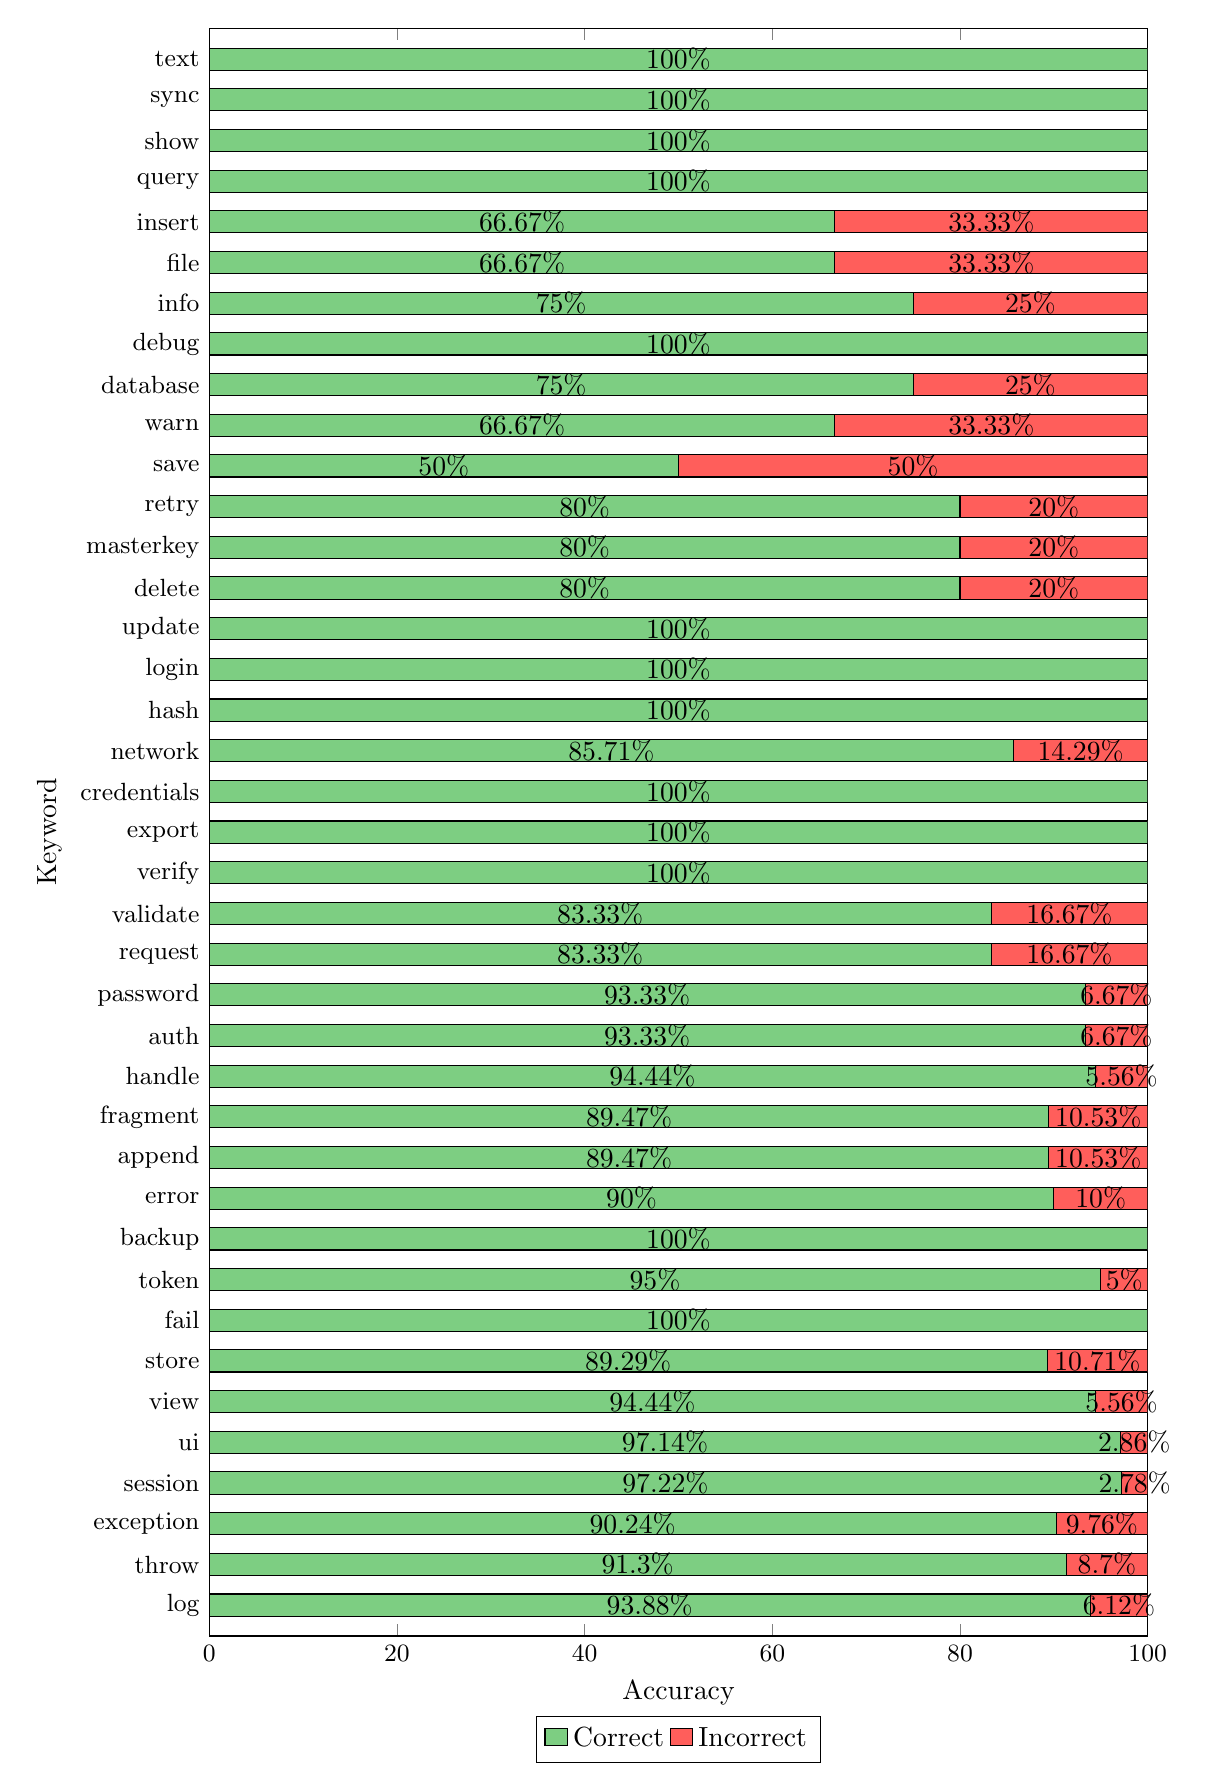
\begin{tikzpicture}
    \begin{axis}[%
      xbar stacked,
      width=13.5cm,height=22cm,
      bar width=8pt,
      symbolic y coords={
        log,throw,exception,session,ui,view,store,fail,token,backup,error,append,
        fragment,handle,auth,password,request,validate,verify,export,credentials,
        network,hash,login,update,delete,masterkey,retry,save,warn,database,
        debug,info,file,insert,query,show,sync,text},
      ytick=data,
      tick label style={font=\small},
      xmin=0,xmax=100,
      xtick={0,20,...,100},
      xlabel={Accuracy},
      ylabel={Keyword},
      nodes near coords={\pgfmathprintnumber[fixed,precision=2]{\pgfplotspointmeta}\%},
      enlarge y limits=0.02,
      legend style={at={(0.5,-0.05)},anchor=north,legend columns=-1},
    ]
      % ─── Correct (green) ────────────────────────────
      \addplot[fill=correct_color] coordinates {
        (93.88,log) (91.30,throw) (90.24,exception) (97.22,session)
        (97.14,ui) (94.44,view) (89.29,store) (100.00,fail)
        (95.00,token) (100.00,backup) (90.00,error) (89.47,append)
        (89.47,fragment) (94.44,handle) (93.33,auth) (93.33,password)
        (83.33,request) (83.33,validate) (100.00,verify) (100.00,export)
        (100.00,credentials) (85.71,network) (100.00,hash) (100.00,login)
        (100.00,update) (80.00,delete) (80.00,masterkey) (80.00,retry)
        (50.00,save) (66.67,warn) (75.00,database) (100.00,debug)
        (75.00,info) (66.67,file) (66.67,insert) (100.00,query)
        (100.00,show) (100.00,sync) (100.00,text)};
      % ─── Incorrect (red) ────────────────────────────
      \addplot[fill=incorrect_color] coordinates {
        ( 6.12,log) ( 8.70,throw) ( 9.76,exception) ( 2.78,session)
        ( 2.86,ui)  ( 5.56,view)  (10.71,store)  ( 0.00,fail)
        ( 5.00,token)( 0.00,backup)(10.00,error) (10.53,append)
        (10.53,fragment)( 5.56,handle)( 6.67,auth) ( 6.67,password)
        (16.67,request)(16.67,validate)( 0.00,verify)( 0.00,export)
        ( 0.00,credentials)(14.29,network)( 0.00,hash)( 0.00,login)
        ( 0.00,update)(20.00,delete)(20.00,masterkey)(20.00,retry)
        (50.00,save) (33.33,warn) (25.00,database)( 0.00,debug)
        (25.00,info) (33.33,file) (33.33,insert)( 0.00,query)
        ( 0.00,show) ( 0.00,sync) ( 0.00,text)};
      \legend{Correct,Incorrect}
    \end{axis}
  \end{tikzpicture}
  \caption{Keyword match accuracy, for version diff A}
  \label{fig:keyword_match_accuracy_A}
\end{figure}



\begin{figure}[H]
  \centering
    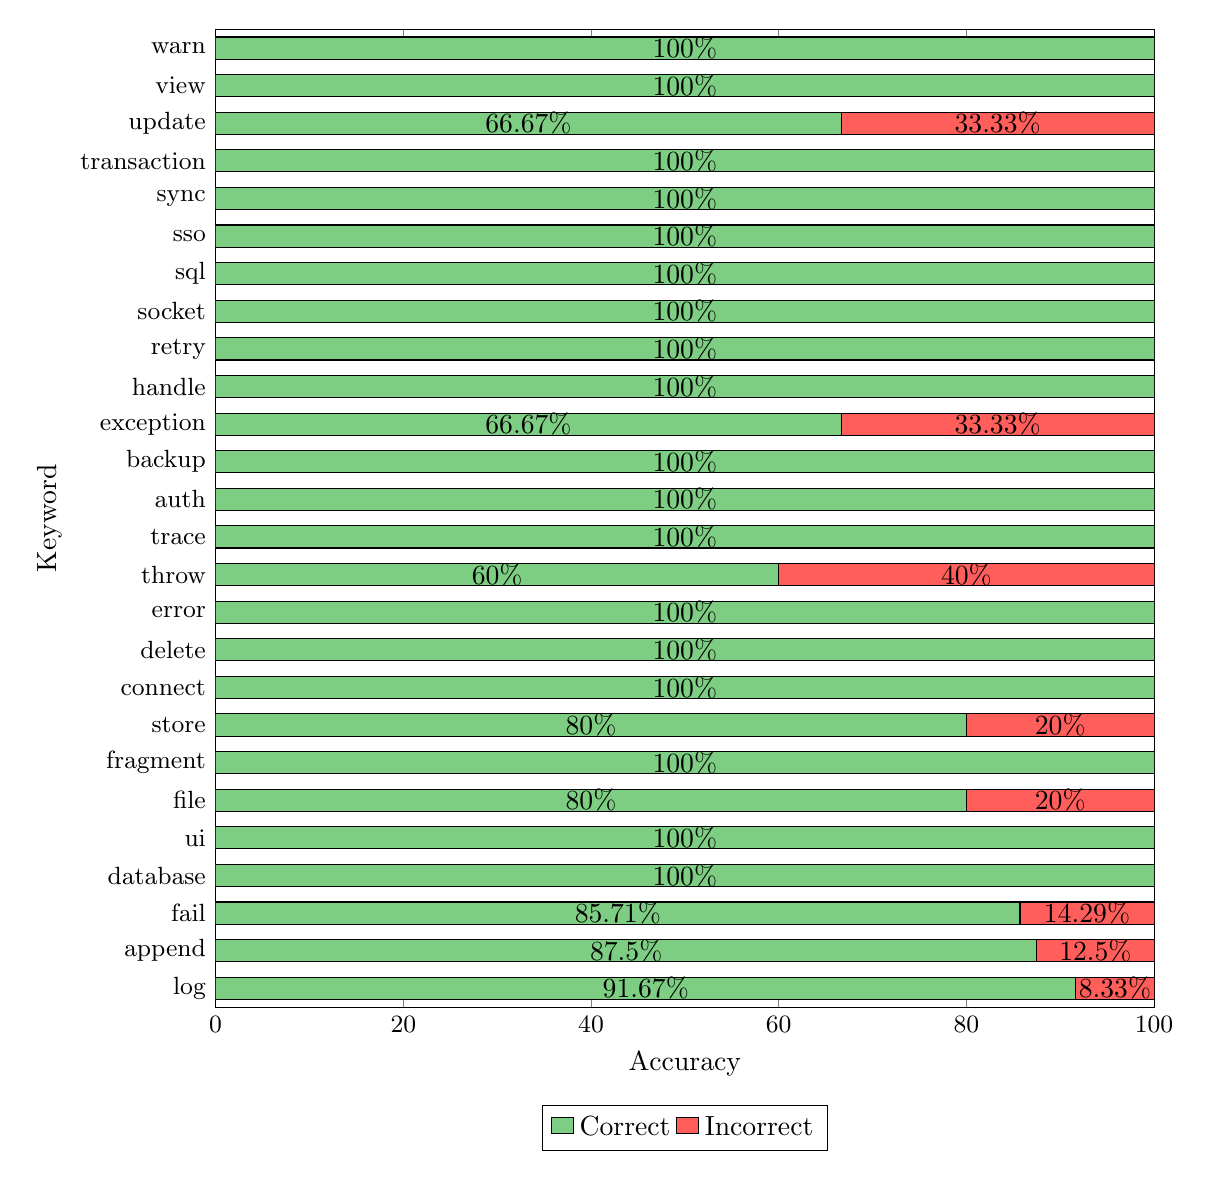
\begin{tikzpicture}
    \begin{axis}[%
      xbar stacked,
      width=13.5cm,height=14cm,
      bar width=8pt,
      symbolic y coords={
        log,append,fail,database,ui,file,fragment,store,connect,delete,error,
        throw,trace,auth,backup,exception,handle,retry,socket,sql,sso,sync,
        transaction,update,view,warn},
      ytick=data,
      tick label style={font=\small},
      xmin=0,xmax=100,
      xtick={0,20,...,100},
      xlabel={Accuracy},
      ylabel={Keyword},
      nodes near coords={\pgfmathprintnumber[fixed,precision=2]{\pgfplotspointmeta}\%},
      enlarge y limits=0.02,
      legend style={at={(0.5,-0.1)},anchor=north,legend columns=-1},
    ]
      % ─── Correct (green) ────────────────────────────
      \addplot[fill=correct_color] coordinates {
        (91.67,log) (87.50,append) (85.71,fail) (100.00,database)
        (100.00,ui) (80.00,file) (100.00,fragment) (80.00,store)
        (100.00,connect) (100.00,delete) (100.00,error) (60.00,throw)
        (100.00,trace) (100.00,auth) (100.00,backup) (66.67,exception)
        (100.00,handle) (100.00,retry) (100.00,socket) (100.00,sql)
        (100.00,sso) (100.00,sync) (100.00,transaction) (66.67,update)
        (100.00,view) (100.00,warn)};
      % ─── Incorrect (red) ────────────────────────────
      \addplot[fill=incorrect_color] coordinates {
         (8.33,log) (12.50,append) (14.29,fail) ( 0.00,database)
         ( 0.00,ui)  (20.00,file)  ( 0.00,fragment) (20.00,store)
         ( 0.00,connect) ( 0.00,delete) ( 0.00,error) (40.00,throw)
         ( 0.00,trace) ( 0.00,auth) ( 0.00,backup) (33.33,exception)
         ( 0.00,handle) ( 0.00,retry) ( 0.00,socket) ( 0.00,sql)
         ( 0.00,sso) ( 0.00,sync) ( 0.00,transaction) (33.33,update)
         ( 0.00,view) ( 0.00,warn)};
      \legend{Correct,Incorrect}
    \end{axis}
  \end{tikzpicture}
  \caption{Keyword match accuracy, for version diff B}
  \label{fig:keyword_match_accuracy_B}
\end{figure}


\begin{figure}[H]
  \centering
    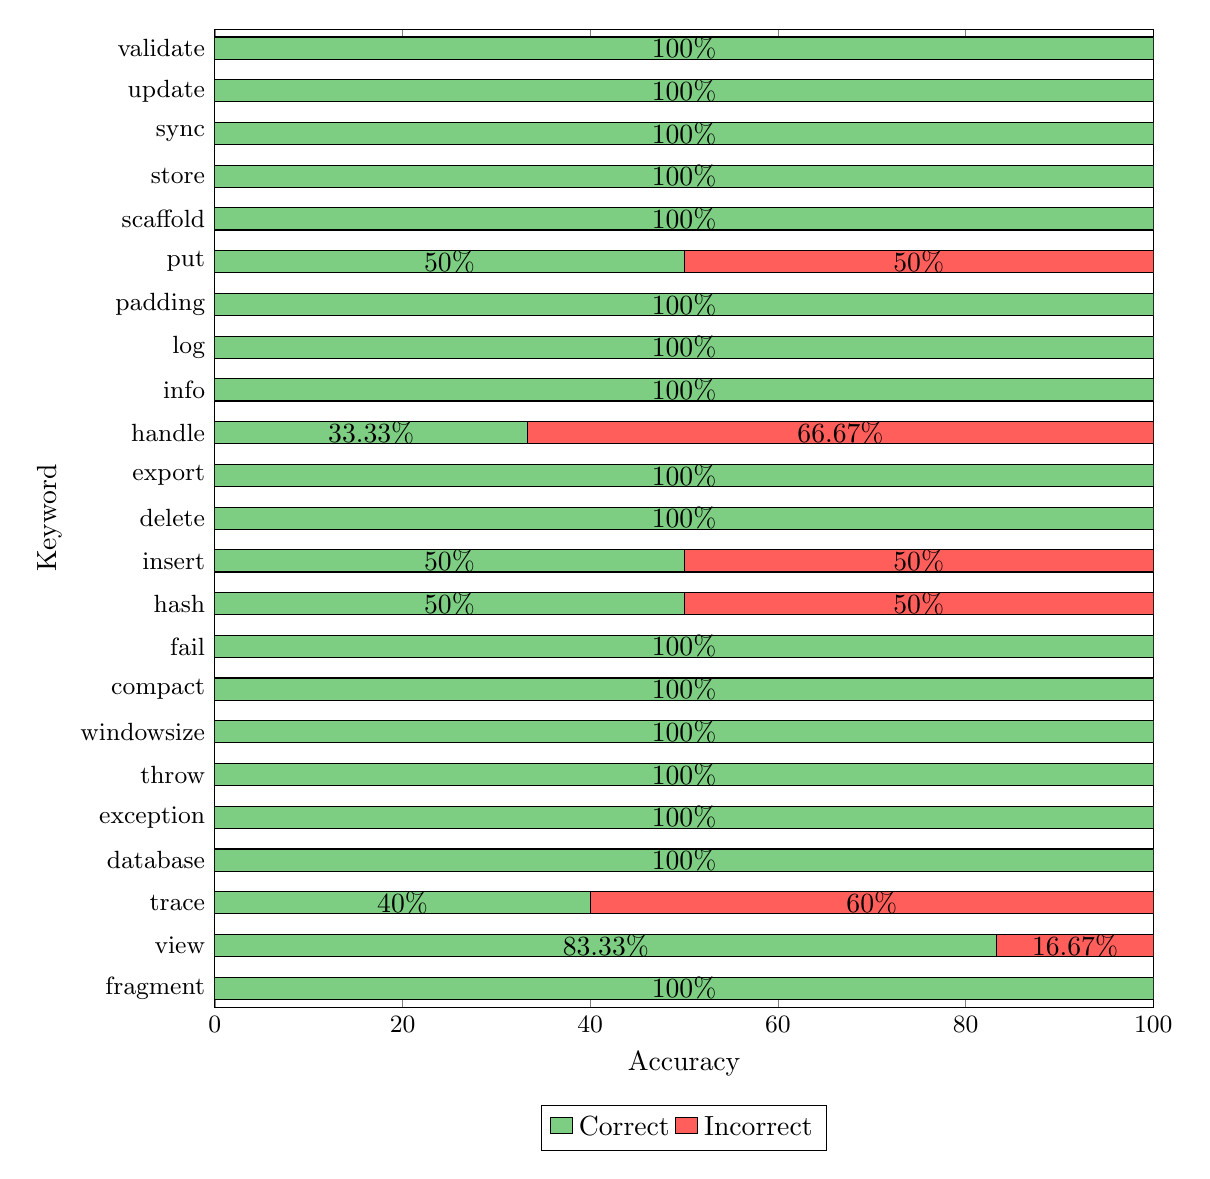
\begin{tikzpicture}
    \begin{axis}[%
      xbar stacked,
      width=13.5cm,height=14cm,
      bar width=8pt,
      symbolic y coords={
        fragment,view,trace,database,exception,throw,windowsize,compact,fail,
        hash,insert,delete,export,handle,info,log,padding,put,scaffold,store,
        sync,update,validate},
      ytick=data,
      tick label style={font=\small},
      xmin=0,xmax=100,
      xtick={0,20,...,100},
      xlabel={Accuracy},
      ylabel={Keyword},
      nodes near coords={\pgfmathprintnumber[fixed,precision=2]{\pgfplotspointmeta}\%},
      enlarge y limits=0.02,
      legend style={at={(0.5,-0.1)},anchor=north,legend columns=-1},
    ]
      % ─── Correct (green) ────────────────────────────
      \addplot[fill=correct_color] coordinates {
        (100.00,fragment) (83.33,view) (40.00,trace) (100.00,database)
        (100.00,exception) (100.00,throw) (100.00,windowsize) (100.00,compact)
        (100.00,fail) (50.00,hash) (50.00,insert) (100.00,delete) (100.00,export)
        (33.33,handle) (100.00,info) (100.00,log) (100.00,padding) (50.00,put)
        (100.00,scaffold) (100.00,store) (100.00,sync) (100.00,update)
        (100.00,validate)};
      % ─── Incorrect (red) ────────────────────────────
      \addplot[fill=incorrect_color] coordinates {
         ( 0.00,fragment) (16.67,view) (60.00,trace) ( 0.00,database)
         ( 0.00,exception) ( 0.00,throw) ( 0.00,windowsize) ( 0.00,compact)
         ( 0.00,fail) (50.00,hash) (50.00,insert) ( 0.00,delete) ( 0.00,export)
         (66.67,handle) ( 0.00,info) ( 0.00,log) ( 0.00,padding) (50.00,put)
         ( 0.00,scaffold) ( 0.00,store) ( 0.00,sync) ( 0.00,update)
         ( 0.00,validate)};
      \legend{Correct,Incorrect}
    \end{axis}
  \end{tikzpicture}
  \caption{Keyword match accuracy, for version diff C}
  \label{fig:keyword_match_accuracy_C}
\end{figure}





%%%%%%%%%%%%%%%%%%%%%%%%%%%%%%
% COMBINED TOTAL RESULT
%%%%%%%%%%%%%%%%%%%%%%%%%%%%%%
\subsection{Comprehensive summary of version diffs}
\label{sec:res:comprehensive_summary}

\subsubsection{Summarized pipeline accuracy}
The table in Figure~\ref{tab:overall_accuracy} presents a comprehensive overview of the pipeline's accuracy, aggregated across all three version differences (diffs). This table provides a summary of the pipeline’s performance in three key aspects:

\begin{itemize}
    \item \textbf{Change Detection Accuracy:} This metric indicates how effectively the pipeline detects changes between the analyzed versions. It is calculated as the proportion of changes identified by the pipeline compared to the total changes identified during the manual analysis.

    \item \textbf{Status Accuracy:} This metric measures the pipeline's ability to correctly determine the status of each detected change—whether it is an addition, modification, or deletion. It reflects how well the pipeline aligns with the manual analysis in classifying the type of each change.

    \item \textbf{Categorization Accuracy:} This metric assesses how accurately the pipeline assigns categories to the detected changes. It is calculated by comparing the categories assigned by the pipeline with those identified during the manual analysis. A correct categorization is counted when the pipeline's assigned categories match or overlap with those determined manually.

\end{itemize}

By aggregating the accuracy results across all three version diffs, this table provides a holistic view of the pipeline’s overall performance. It helps identify strengths and weaknesses in the change detection, status classification, and categorization processes, offering valuable insights for further improvement.


\begin{comment}
FOUND ACCURACY = (81+21+26)/(84+28+28) = 0,9142857143
STATUS ACCURACY = (71+16+23)/(84+28+28) = 0,7857142857

TOT CATEGORY ACCURACY = (72+17+15)/(84+28+28) = 0,7428571429
CATEGORY ACCURACY CRITICAL = (48+9+3)/(57+16+4) = 0,7792207792
CATEGORY ACCURACY NON-CRIT = (24+8+12)/(27+12+24) = 0,6984126984
\end{comment}

\begin{table}[H]
    \centering
    \begin{tabular}{l l}
        \toprule
        \textbf{Metric} & \textbf{Accuracy} \\
        \midrule
        Changes detected & 91.4\% \\
        Correct change status & 78.6\% \\
        Correctly set categories & 74.3\% \\
        \textit{\ \ \ \ \ \ \ \ Critical categories} & 77.9\% \\
        \textit{\ \ \ \ \ \ \ \ Non-critical categories} & 69.8\% \\
        \bottomrule
    \end{tabular}
    \caption{Combined pipeline accuracy metrics.}
    \label{tab:overall_accuracy}
\end{table}


\subsubsection{Summarized Category Assignment Accuracy}

As previously mentioned in Section~\ref{sec:result:categorization_distributions:categories_resulting_in_correct_incorrect_categorizations}, the categories \codebox{UI update} and \codebox{Authentication} demonstrated the highest accuracy in correct category assignments. This observation is further supported by the detailed accuracy analysis presented in Figures~\ref{fig:correct_incorrect_categorization_accuracy_critical} and \ref{fig:correct_incorrect_categorization_accuracy_noncritical}, which provide a clear view of the correct and incorrect categorization rates for each category.

A closer look at these figures reveals that some categories, such as \codebox{File write}, \codebox{Cryptographic}, and \codebox{Text manipulation}, exhibit 0\% accuracy in correct assignments. However, this result is misleading because the total number of assignments for these categories is either extremely low or nonexistent. Consequently, even a single incorrect categorization can significantly skew the accuracy percentage for these categories.

Additionally, the category \codebox{Error handling} shows consistently low accuracy, even though it has a substantial number of assignments, both correct and incorrect. This suggests that the categorization keywords associated with \codebox{Error handling} may require refinement to improve accuracy.

From these observations, it is clear that the critical categories \codebox{Authentication} and \codebox{Data storage}, along with the non-critical categories \codebox{UI update} and \codebox{Network call}, have keyword definitions that are highly effective in producing accurate and reliable categorizations. These categories benefit from well-defined and contextually relevant keywords, leading to consistent and correct classifications. High accuracy of the non-critical categories like \codebox{UI update} and \codebox{Network call} is beneficial when analyzing the tool's report. Accurately filtering out unimportant changes reduces the number of critical changes to investigate, making the manual review process more focused and efficient.


\begin{table}[H]
    \centering

    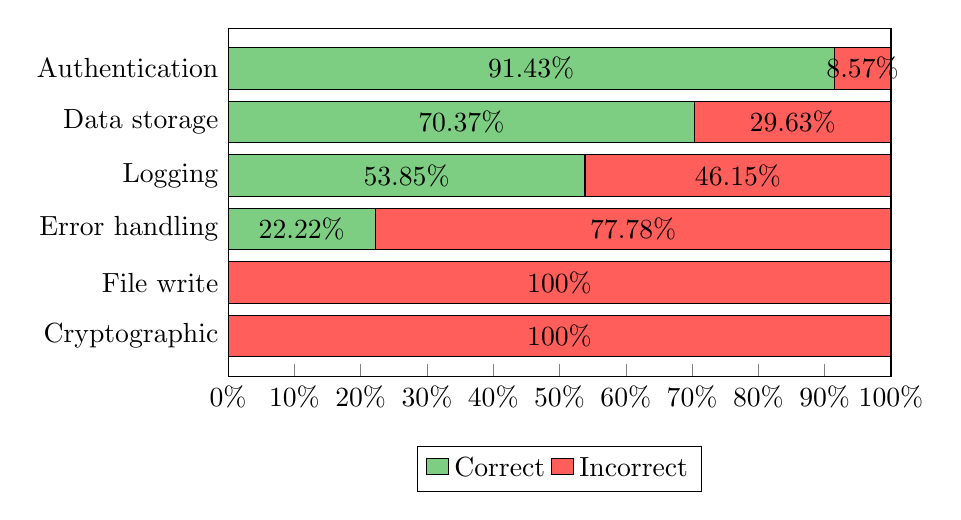
\begin{tikzpicture}
        \begin{axis}[%
        xbar stacked,
        width=10cm,height=6cm,
        bar width=15pt,
        %
        % ── value labels ────────────────────────────────
        nodes near coords={\pgfmathprintnumber[fixed,precision=2]{\pgfplotspointmeta}\%},
        %
        xmin=0,xmax=100,
        xtick={0,10,...,100},
        ytick={1,...,6},
        yticklabels={
          Cryptographic,
          File write,
          Error handling,
          Logging,
          Data storage,
          Authentication},
        xtick pos=bottom,
        ytick pos=left,
        xticklabel={\pgfmathprintnumber[fixed,precision=2]{\tick}\%},
        enlarge y limits=.15,
        legend style={at={(0.5,-0.20)},anchor=north,legend columns=-1},
        ]
        % ─── Correct (green) ────────────────────────────
        \addplot[xbar,fill=correct_color] coordinates {
          (0,1) (0,2) (22.22,3) (53.85,4) (70.37,5) (91.43,6)};
        % ─── Incorrect (red) ────────────────────────────
        \addplot[xbar,fill=incorrect_color] coordinates {
          (100,1) (100,2) (77.78,3) (46.15,4) (29.63,5) (8.57,6)};
        \legend{Correct,Incorrect}
        \end{axis}
    \end{tikzpicture}
    
    \caption{Total ratio of correct vs incorrect assignment of critical categories.}
    \label{fig:correct_incorrect_categorization_accuracy_critical}
\end{table}


\begin{table}[H]
    \centering

    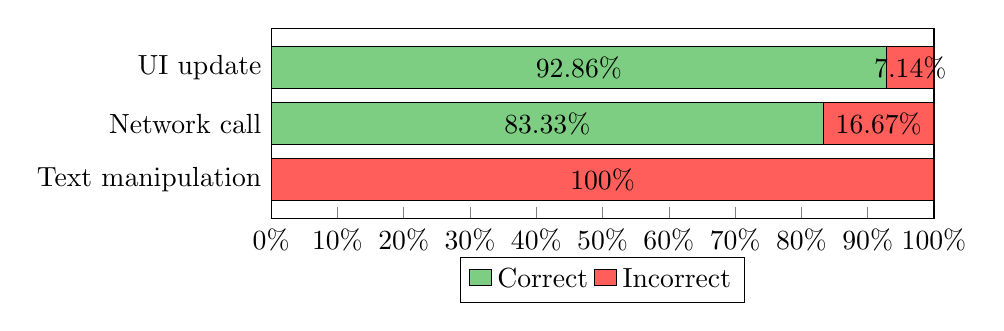
\begin{tikzpicture}
        \begin{axis}[%
        xbar stacked,
        width=10cm,height=4cm,
        bar width=15pt,
        %
        % ── value labels ────────────────────────────────
        nodes near coords={\pgfmathprintnumber[fixed,precision=2]{\pgfplotspointmeta}\%},
        %
        xmin=0,xmax=100,
        xtick={0,10,...,100},
        ytick={1,...,3},
        yticklabels={
          Text manipulation,
          Network call,
          UI update},
        xtick pos=bottom,
        ytick pos=left,
        xticklabel={\pgfmathprintnumber[fixed,precision=2]{\tick}\%},
        enlarge y limits=0.35,
        legend style={at={(0.5,-0.20)},anchor=north,legend columns=-1},
        ]
        % ─── Correct (green) ────────────────────────────
        \addplot[xbar,fill=correct_color] coordinates {
          (0,1) (83.33,2) (92.86,3)};
        % ─── Incorrect (red) ────────────────────────────
        \addplot[xbar,fill=incorrect_color] coordinates {
          (100,1) (16.67,2) (7.14,3)};
        \legend{Correct,Incorrect}
        \end{axis}
    \end{tikzpicture}
    
    \caption{Total ratio of correct vs incorrect assignment of non-critical categories.}
    \label{fig:correct_incorrect_categorization_accuracy_noncritical}
\end{table}

%%% Discussion.tex --- 
%% 
%% Filename: Discussion.tex
%% Author: Jacob Ringfjord & Max Wilén
%%% Code:

\chapter{Discussion}
\label{cha:discussion}
This chapter begins by reviewing the findings presented in chapter \ref{cha:result} \textit{Result}, focusing on the performance and accuracy of the categorization. Secondly, the method from \ref{cha:methodology} \textit{Methodology} is discussed by reflecting on its design, implementation, and limitations. Lastly, the chapter explores the wider context of this thesis, considering the societal implications of the work. 

\section{Results}
\label{sec:discussion-results}
\begin{comment}
\begin{itemize}
    \item Best/worst categorization type accuracy
    \item False positive and false negatives
    
    \item in some cases the pipeline analysis can actually be more precise and correct than the manual analysis since the pipeline processes operations done in the execution flow, and the manual analysis has only looked at the specific code line and it surrounding code lines to get a general view of what is happening. (more categories chosen by the pipeline than the manual analysis does not mean that the pipeline is too broad and too easily sets a category).
    
    \item in version diff C: more than usual amount of faulty categorizations. a lot of the manual analysis done detected UI changes, but the pipeline detected some other category. This could be because, only for this specific version diff, because the changes seemed when looking at the source code to indicate simple UI changes (viewmodel, mainactivity, onCreate etc) that was thought to not create any critical changes. this hypothesis can however be wrong since the pipeline seems to uncover more information/operations connected to the change that points to a critical change actually occuring. Therefore, this lack of high accuracy for this version diff could instead point to the pipeline being more effective at finding critical differences than the human eye (only looking at a specific code line)
\end{itemize}



One distinguishing factor between the manual evaluation process used for obtaining the results and the output from the developed tool is that the latter considers the program's control flow. The manual analysis relies on us investigating the changes in the source code and only reviewing them on an individual level. An approach where a more sophisticated investigation was made, where the usage was overseen, etc. would affect the consistency of the method since it would be difficult to treat everything equally. It would also be very time-consuming to do this for every change. However, the developed tool analyses the control flow of the program when comparing the given binaries and detecting the changes. Therefore, the analysis derived from the tool may sometimes be more precise than the manual analysis, since it analyzes from a more in-depth perspective. This is interesting since the accuracy of the pipeline in some cases may be more precise than the manual analysis if the latter one is categorized incorrectly.




MAX TANKAR:
    the subjective nature of the manual analysis:
    - is a correct categorization actually correct?
    

\begin{enumerate}
    \item[Is a correct categorization actually correct?] Is the categorization too lenient—are too many changes being assigned to the most critical categories?
    
    - categorizations being marked as correct even though the majority of the categories marked by the pipeline is not part of the manual analysis.
    
    KLAR - too many changes marked with a majority of the critical categories? can both be a consequence of the pipeline looking at execution flow (good consequence), and that the categorization is too kind (bad consequence).
    
\end{enumerate}
\end{comment}

Following the result presented in Chapter \ref{cha:result}, two main points of interest for further discussion have come up. The two are split up for the reason of targeting different root concerns, but they do somewhat intersect with each other:

\begin{explanation}
    These are addressed in their respective subsections.
    \begin{enumerate}
        \item \textbf{Effective neglection of less important changes} - Why does high categorization accuracy of \textit{non-critical} changes provides great value?
        
        \item \textbf{Validity of the categorization} - How confident can we be that each change has been placed in the correct category?
    
        \item \textbf{Criteria for correctness} – What threshold or standard determines whether a categorization is judged correct or incorrect?

        \item \textbf{Depth of coverage} - Are all categories and keywords adequately represented in the result data to yield reliable accuracy estimates?
    \end{enumerate}
\end{explanation}

\subsection{Effective neglection of less important changes}
At a first glance of the result presented in Chapter \ref{cha:result}, it is clear that accurate categorization of \emph{critical} changes is essential when detecting differences between two versions. However, while developing this novel approach to change categorization, we also recognized that high accuracy in identifying \emph{non‑critical} changes can filter out modifications that would otherwise distract analysts from the issues that matter most. Because of this, it is wise to acknowledge this fact when considering both usage of the tool and future development.


\subsection{Validity of the Categorization}
\label{sec:discussion:result:validity_of_categorization}
As presented in Section \ref{sec:res:categorization_result:manual_evaluation_process}, the way that the declaration of a correct/incorrect categorization is done in this thesis has its accompanied concerns. Most obviously is the reliability of the manual analysis being correct in the first place, but this is discussed in the upcoming Section \ref{sec:discussion:subjective_nature_manual_analysis}. 

% many critical changes received a majority if the critical categories
% bad take ->
Instead, we highlight the issue that many critical changes are assigned to several critical categories. Put differently, a substantial share of changes flagged as critical during the manual review have been assigned several critical categories by the pipeline, even though the manual analysis associated each with only a few. This is concerning because it is unclear whether the manual review was incorrect in the first place or whether the pipeline’s categorization is overly generous. It could be that the keyword lists for each category might need to be shortened, or a more relational keyword-matching approach—one that considers the relative positions of keywords—could produce more reliable results.  However, that is not part of this thesis.

% good take ->
Viewed from another angle, the pipeline’s seemingly “generous” labeling might simply reflect a higher level of accuracy and detail than the manual review. Because the pipeline bases its classifications on function-level data derived from Ghidra’s control-flow analysis, it evaluates not only the operations directly modified by a change but also the downstream operations influenced by that change and the overall structure that the change produces. Because of this, changes that have been assigned more categories by the pipeline analysis than the manual analysis can be a consequence of the manual analysis being too vague.



\subsection{Criteria for correctness}
This section examines the standards for calling a categorization correct or incorrect when we compare the manual review with the pipeline’s output, and it highlights the limitations of that comparison.

The current method counts a change as “correctly categorized” even when the pipeline matches only a subset of the categories identified in the manual review. This can distort the results: a change tagged with all categories by the pipeline may still be labeled correct even though the manual analysis assigned just one. As noted in Section \ref{sec:discussion:result:validity_of_categorization}, the mismatch may stem from the pipeline’s finer granularity, but it is still problematic. Many changes end up marked as fully correct when they would be better described as e.g., only \textit{partly correct}. However, we decided not to adapt such labeling because it might add complexity without improving reliability. At the time of writing this thesis, we cannot tell whether the pipeline, the manual review, or both contains the greater inaccuracy, so we lack a clear basis for weighting one over the other. Given this uncertainty—and the experimental nature of the thesis—we have maintained the existing approach. Future studies may shed more light on the issue, with this thesis approach in mind.



\subsection{Depth of coverage}
Looking at the results in Chapter \ref{cha:result}, it is clear that some categories—\codebox{File write}, \codebox{Cryptographic}, and \codebox{Text manipulation}—are under-represented, so their performance metrics cannot be considered reliable. In contrast, the many assignments to \codebox{UI update} and \codebox{Data storage} indicate that the selected version diffs are weighted toward changes that primarily affect those categories. With this in mind, it would—for future additions to this work—be of interest how to choose test data that more effectively targets all the categories used as part of the categorization. Unfortunately, this lies beyond the scope of this thesis.






\subsection{Limitations}

\begin{comment}
\textbf{TODO:} Full category metric score is given to a function that has all the categories listed in the hypothesis in the pipeline result column. So, if there is an extra category in the pipeline result which is not found in the hypothesis, this still is considered a full point.

\textbf{TODO:} code diff syntax analysis is only computed for the critical categories. some explanation has been done in the method (regex explanation), but more is probably needed.

\begin{itemize}
    \item Multiple detections for same change
    \item Alot more detections and category hits detected by the pipeline than discovered through the manual analysis. The accuracy calculations follows because of this from a small subset of the changes detected by the pipeline.
\end{itemize}    
\end{comment}

Challenges arise in reverse engineering when the analyzed code does not accurately reflect the original functionality. For instance, when stripped binaries or obfuscated code are used. These techniques hinder reverse engineers by removing or altering meaningful code structures, such as function names and symbols.

Such cases have not been studied in this thesis. The pipeline heavily relies on the assumption that the output from Ghidriff reflects the program's true functionality. If the categorization is performed on tampered code like this, it may have a significant impact on the accuracy of the result. This represents a key limitation of the thesis, which is difficult to overcome.

\section{Method}
\label{sec:discussion-method}

Building on the results in Chapter \ref{cha:result} and the methodology in Chapter \ref{cha:methodology}, we have identified several discussion points. Each one stems from a different core concern, yet they partly overlap. 

\begin{explanation}
    These are addressed in their respective subsections.
    \begin{enumerate}    
        \item \textbf{Uncontrollable external deficiencies} - How do external actions affect the pipeline?

        \item \textbf{Subjective Nature of a Manual Analysis} - How certain can we be that the manual analysis was done correctly?

        \item \textbf{Choice of Test Data} - Is Signal an appropriate program for testing the pipeline?

    \end{enumerate}
\end{explanation}

\subsection{Uncontrollable external deficiencies}
This thesis utilizes the previously mentioned tool, Ghidriff, to detect the changes between different software versions. As shown in Table \ref{tab:overall_accuracy}, not all changes are successfully detected from Ghidriff. If this is due to limitations in Ghidra or Ghidriff is unknown and falls outside the scope of this thesis to investigate, but it does affect the result. It is worth mentioning that Ghidriff has only been referenced in a limited number of prior studies, which may indicate that its capabilities and limitations are not fully explored. In this thesis, there have been cases where Ghidriff has not been able to analyze all .dex files, which can be seen in Table \ref{tab:run_time}.


\subsection{Subjective Nature of a Manual Analysis}
\label{sec:discussion:subjective_nature_manual_analysis}
The results presented in this thesis are derived through manual analysis, and the source code is analyzed without prior knowledge of the implementation. Since both the source code and the output from the pipeline tool are based on this approach, there is a potential for bias. For instance, manual examination of the source code can present challenges since the implementation can sometimes be difficult to understand without knowing the entire code base. This highlights the subjective nature of the manual analysis. To counter this, an approach where a more sophisticated manual analysis was made would increase the consistency and reliability, but would also be more time-consuming, given the complexity of automating such a task.

The results presented in this thesis rest on the prior assumption that a change behaves as interpreted when one examines the specific line of code. Commit messages linked to the change can lend some support to this assumption, but the precise reason the change occurred remains uncertain, and the findings must therefore be interpreted with this limitation in mind.


\subsection{Choice of Test Data}
Testing has only been performed with the Android version of Signal, as presented in previous chapters. The reason for this lies in two main reasons. First, the NFC specifically requested Signal-Android because its scale and architectural style resemble the other apps they plan to process with the pipeline, making it a practical and representative choice for initial testing. Second, Signal’s open-source codebase simplifies data collection and analysis.

% The results from the three version diffs analyzed in this thesis may not represent other applications in the same field. However, Signal was chosen since it is a large-scale application and an interesting one for the client to investigate. It is also one of the few where the source code is publicly accessible, which is required in this thesis to validate the performance of the developed tool.


\begin{comment}
\subsection{Why we chose Ghidriff}

\textbf{NOTE TO SULEMAN:} Not sure if this is needed? Some explanation can be found in Chapter \ref{cha:methodology}, but maybe that is not enough?
\end{comment}


\section{Replicability}
\label{sec:replicability}
To replicate the research performed in this thesis, the pipeline tool described in Chapter \ref{cha:methodology} must be used. The tool and additional information regarding installation and setup are accessible from the thesis project's GitHub repository \cite{public_project_github}. All Signal versions mentioned in the thesis are public releases retrieved from the Signal GitHub repository \cite{githubSignal}. Lastly, Section \ref{sec:res:categorization_result:manual_evaluation_process} describes how the manual evaluation was conducted to collect the results in this thesis.

\section{The Work in a Wider Context}
\label{sec:work-wider-context}
This thesis has been conducted on behalf of a client operating in the digital forensics sector. The tool
has been tailored to meet their needs and requirements, but has been developed with flexibility in mind. The categories and keywords used can easily be modified, making it adaptable for a wider range of usage beyond its original purpose. 

\subsection{Ethical Considerations}
In the context of digital forensics, there are two opposing perspectives: those who aim to exploit systems and those who work to protect and investigate them. Therefore, ethical considerations remain an important aspect of this thesis. A potential hacker could benefit from understanding the differences between two software versions, as such changes may introduce new vulnerabilities that could be exploited in recently released software.

However, the tool developed in this thesis is intended to streamline the process of selecting appropriate forensic methods for the client and not replace it. Based on the results obtained and insights gained from the analysis, the tool does not appear to be sufficient on its own for use in malicious activities such as hacking. Manual reverse-engineering and use of additional, more specialized software still seem necessary. While a skilled hacker might find value in the information provided by the tool, they would likely already have access to more effective tools suited for such purposes. All development in this thesis has been carried out using publicly available tools for everyone to use. 

%%% Conclusion.tex --- 
%% 
%% Filename: Conclusion.tex
%% Author: Jacob Ringfjord & Max Wilén
%%% Code:

\chapter{Conclusion}
\label{cha:conclusion}

This thesis presents a novel method for categorizing changes in Android binaries across different software versions. The outcome of this work is a tool designed to streamline reverse engineering processes through a set of targeted features.

The result showed that the tool detected 91.4\% of the changes, with a categorization accuracy of 74.3\%. Across the three release comparisons, only 3.3\% of the unique changes were marked as \textit{uncategorized}, indicating they did not match any of the defined categories. Among the critical changes, the pipeline performed best on \textit{Authentication} changes, with an accuracy of 91.43\%, followed by \textit{Data storage} at 70.47\%. For non-critical changes, the accuracy was 92.86\% for \textit{UI updates} and 83.33\% for \textit{Network calls}, demonstrating that these less important changes can be filtered out with reasonable effectiveness, resulting in a smaller and more focused set of critical changes for manual analysis.

In addition to the presented results of the tool's performance and accuracy, the following research questions have been answered:

\begin{enumerate}
\item{\textbf{How does forensic analysis depend on knowledge of the differences between different versions of software applications?}}
\newline
...

\item{\textbf{How to effectively determine programmatical changes of an Android application, based only
on the executable?}}
\newline
...

\item{\textbf{What techniques are most suitable for performing categorization of changes?}}
\newline
...
\end{enumerate}


\section{Future work}
\begin{comment}
    add callgraphs to the pipeline report?
    - https://clearbluejar.github.io/posts/callgraphs-with-ghidra-pyhidra-and-jpype/
\end{comment}
There are several directions for extending the research presented in this thesis. The most significant challenge discovered throughout the project is the time-consuming manual evaluation process for verifying the result. In this thesis, three version diffs were investigated; a more comprehensive analysis would require more comparisons. Automating this process could not only improve the efficiency of gathering more results but also remove the human bias in the source code evaluation. 

Furthermore, with additional data from the pipeline analysis, the use of machine learning and training larger data sets is an interesting path to explore. While the current state of the tool can determine whether a change is related to a specific category, it cannot differentiate between clear and ambiguous cases.

An alternative approach is to work recursively with the provided call graphs from Ghidra, by categorizing the preceding functions that lead to the actual change. This would introduce an additional step beyond the current syntax matching, making the categorization method more advanced. While this process can be performed manually, integrating it into the tool would significantly improve its efficiency. 

%%%%%%%%%%%%%%%%%%%%%%%%%%%%%%%%%%%%%%%%%%%%%%%%%%%%%%%%%%%%%%%%%%%%%%
%%% lorem.tex ends here

%%% Local Variables: 
%%% mode: latex
%%% TeX-master: "demothesis"
%%% End: 


\printbibliography
%%% Appendix.tex --- 
%% 
%% Filename: Appendix.tex
%% Author: Jacob Ringfjord & Max Wilén
%%% Code:


\begin{appendices}
\chapter{Appendix}
\newpage

\begin{figure}[H]
    \centering
    \lstinputlisting[language=json]{code_blocks/ghidriff_json_output.json}
    \caption{Ghidriff output in JSON format from Signal v7.34.2 and v7.35.0}
    \label{fig:ghidriff_json_output_A}
\end{figure}

\begin{figure}[H]
    \centering
    \lstinputlisting[language=json]{code_blocks/ghidriff_json_output_2.json}
    \caption{Ghidriff output in JSON format from Signal v7.34.2 and v7.35.0}
    \label{fig:ghidriff_json_output_B}
\end{figure}

\begin{figure}[H]
    \centering
    \lstinputlisting[language=json]{code_blocks/ghidriff_json_output_3.json}
    \caption{Ghidriff output in JSON format from Signal v7.34.2 and v7.35.0}
    \label{fig:ghidriff_json_output_C}
\end{figure}

\begin{comment}
\begin{figure}[H]
    \centering
    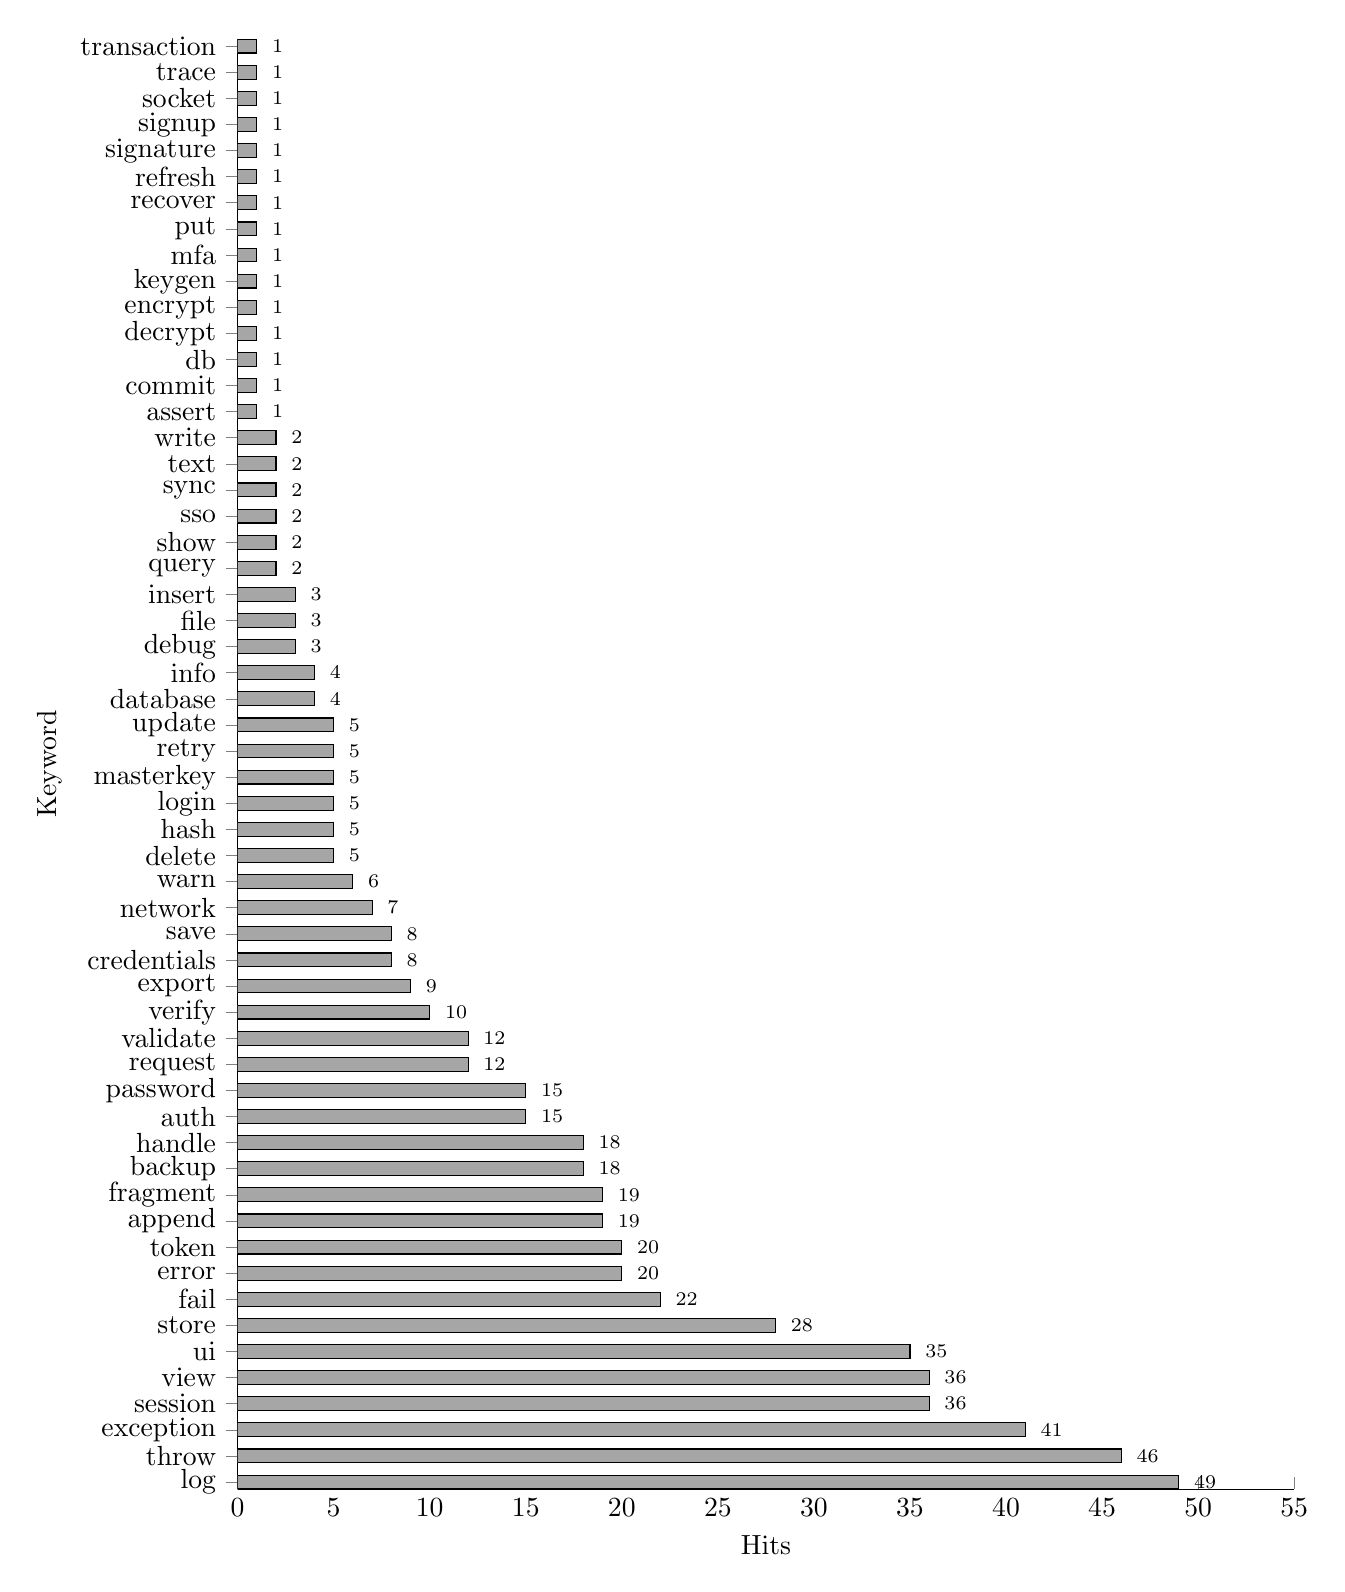
\begin{tikzpicture}
      \begin{axis}[
        width=15cm,
        height=20cm,
        xbar,
        bar width=5pt,
        symbolic y coords={
            log,throw,exception,session,view,ui,store,fail,error,token,
            append,fragment,backup,handle,auth,password,request,validate,
            verify,export,credentials,save,network,warn,delete,hash,login,
            masterkey,retry,update,database,info,debug,file,insert,query,
            show,sso,sync,text,write,assert,commit,db,decrypt,encrypt,
            keygen,mfa,put,recover,refresh,signature,signup,socket,trace,
            transaction},
        ytick=data,
        tick label style={font=\normalsize},
        enlarge y limits=0.005,
        xlabel={Hits},
        ylabel={Keyword},
        xmin=0, xmax=55,
        nodes near coords,
        every node near coord/.append style={font=\scriptsize,xshift=2pt},
        axis x line*=bottom,
        axis y line*=left
      ]
        \addplot[xbar,fill=gray!70] coordinates {
          (49,log) (46,throw) (41,exception) (36,session) (36,view)
          (35,ui) (28,store) (22,fail) (20,error) (20,token)
          (19,append) (19,fragment) (18,backup) (18,handle)
          (15,auth) (15,password) (12,request) (12,validate)
          (10,verify) (9,export) (8,credentials) (8,save)
          (7,network) (6,warn) (5,delete) (5,hash) (5,login)
          (5,masterkey) (5,retry) (5,update) (4,database)
          (4,info) (3,debug) (3,file) (3,insert) (2,query)
          (2,show) (2,sso) (2,sync) (2,text) (2,write)
          (1,assert) (1,commit) (1,db) (1,decrypt) (1,encrypt)
          (1,keygen) (1,mfa) (1,put) (1,recover) (1,refresh)
          (1,signature) (1,signup) (1,socket) (1,trace)
          (1,transaction)
        };
      \end{axis}
    \end{tikzpicture}
    \caption{All keyword hits generating categorizations in version diff A}
    \label{fig:commonly_used_words_A_full_sorted}
\end{figure}


\begin{figure}[H]
    \centering
    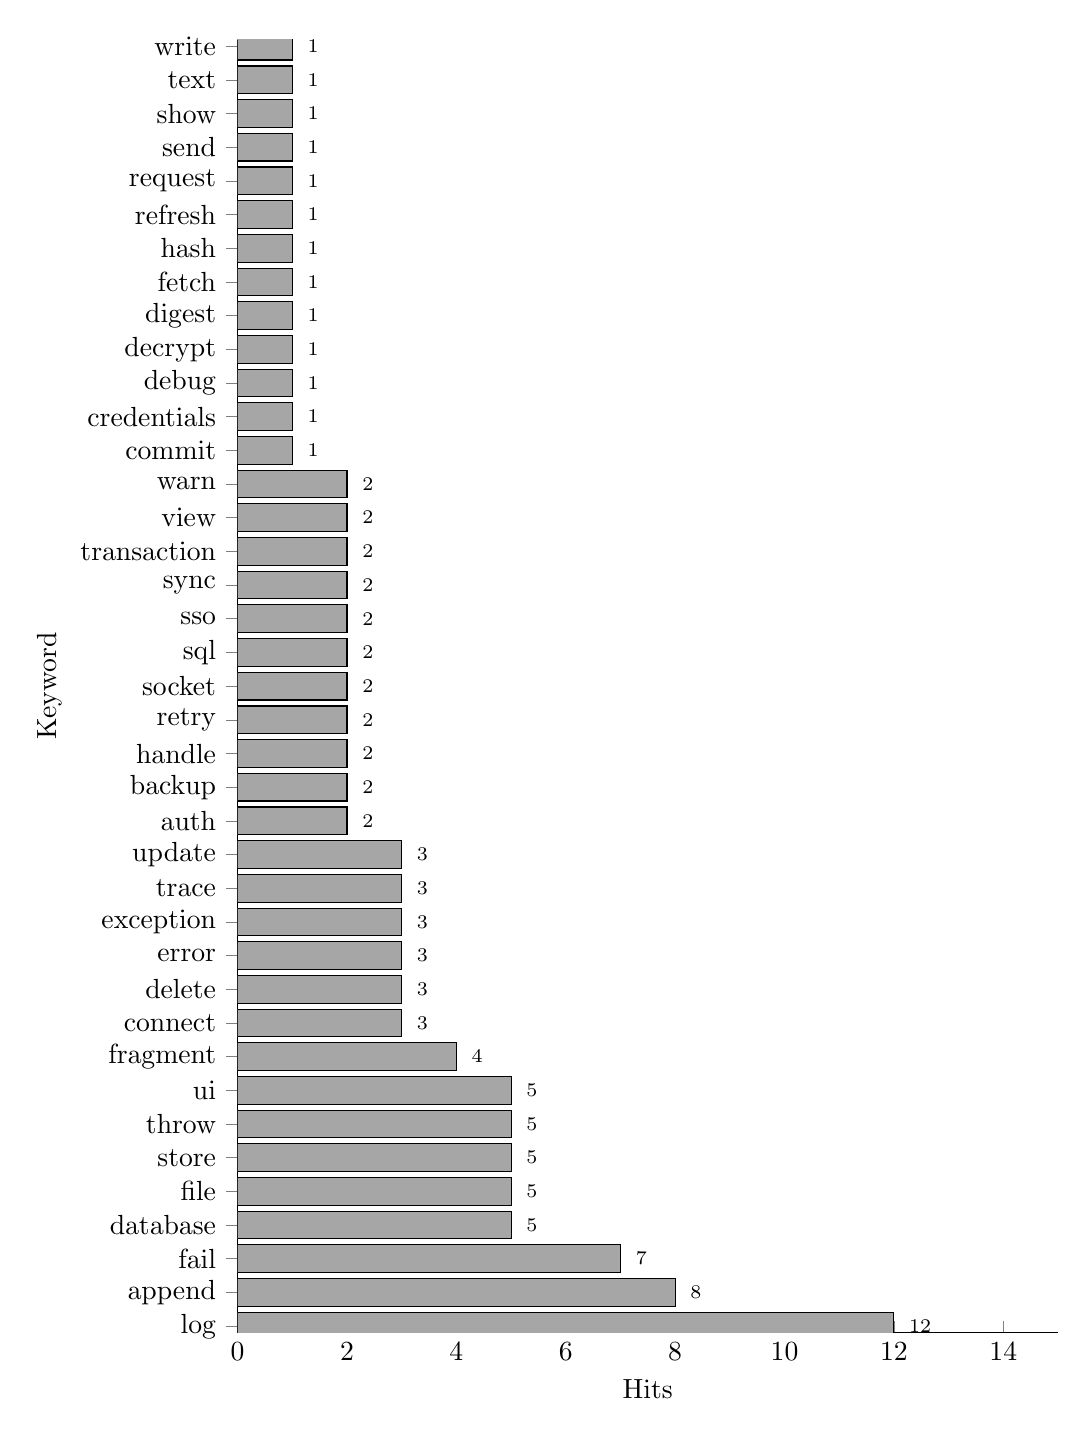
\begin{tikzpicture}
      \begin{axis}[
        width=12cm,
        height=18cm,
        xbar,
        bar width=10pt,
        symbolic y coords={
            log,append,fail,database,file,store,throw,ui,fragment,connect,
            delete,error,exception,trace,update,auth,backup,handle,retry,
            socket,sql,sso,sync,transaction,view,warn,commit,credentials,
            debug,decrypt,digest,fetch,hash,refresh,request,send,show,text,
            write},
        ytick=data,
        tick label style={font=\normalsize},
        enlarge y limits=0.005,
        xlabel={Hits},
        ylabel={Keyword},
        xmin=0, xmax=15,
        nodes near coords,
        every node near coord/.append style={font=\scriptsize,xshift=2pt},
        axis x line*=bottom,
        axis y line*=left
      ]
        \addplot[xbar,fill=gray!70] coordinates {
          (12,log) (8,append) (7,fail) (5,database) (5,file) (5,store)
          (5,throw) (5,ui) (4,fragment) (3,connect) (3,delete) (3,error)
          (3,exception) (3,trace) (3,update) (2,auth) (2,backup) (2,handle)
          (2,retry) (2,socket) (2,sql) (2,sso) (2,sync) (2,transaction)
          (2,view) (2,warn) (1,commit) (1,credentials) (1,debug) (1,decrypt)
          (1,digest) (1,fetch) (1,hash) (1,refresh) (1,request) (1,send)
          (1,show) (1,text) (1,write)
        };
      \end{axis}
    \end{tikzpicture}
    \caption{All keywords hits generating categorizations in version diff B}
    \label{fig:commonly_used_words_B_full_rotated}
\end{figure}

\begin{figure}[H]
    \centering
    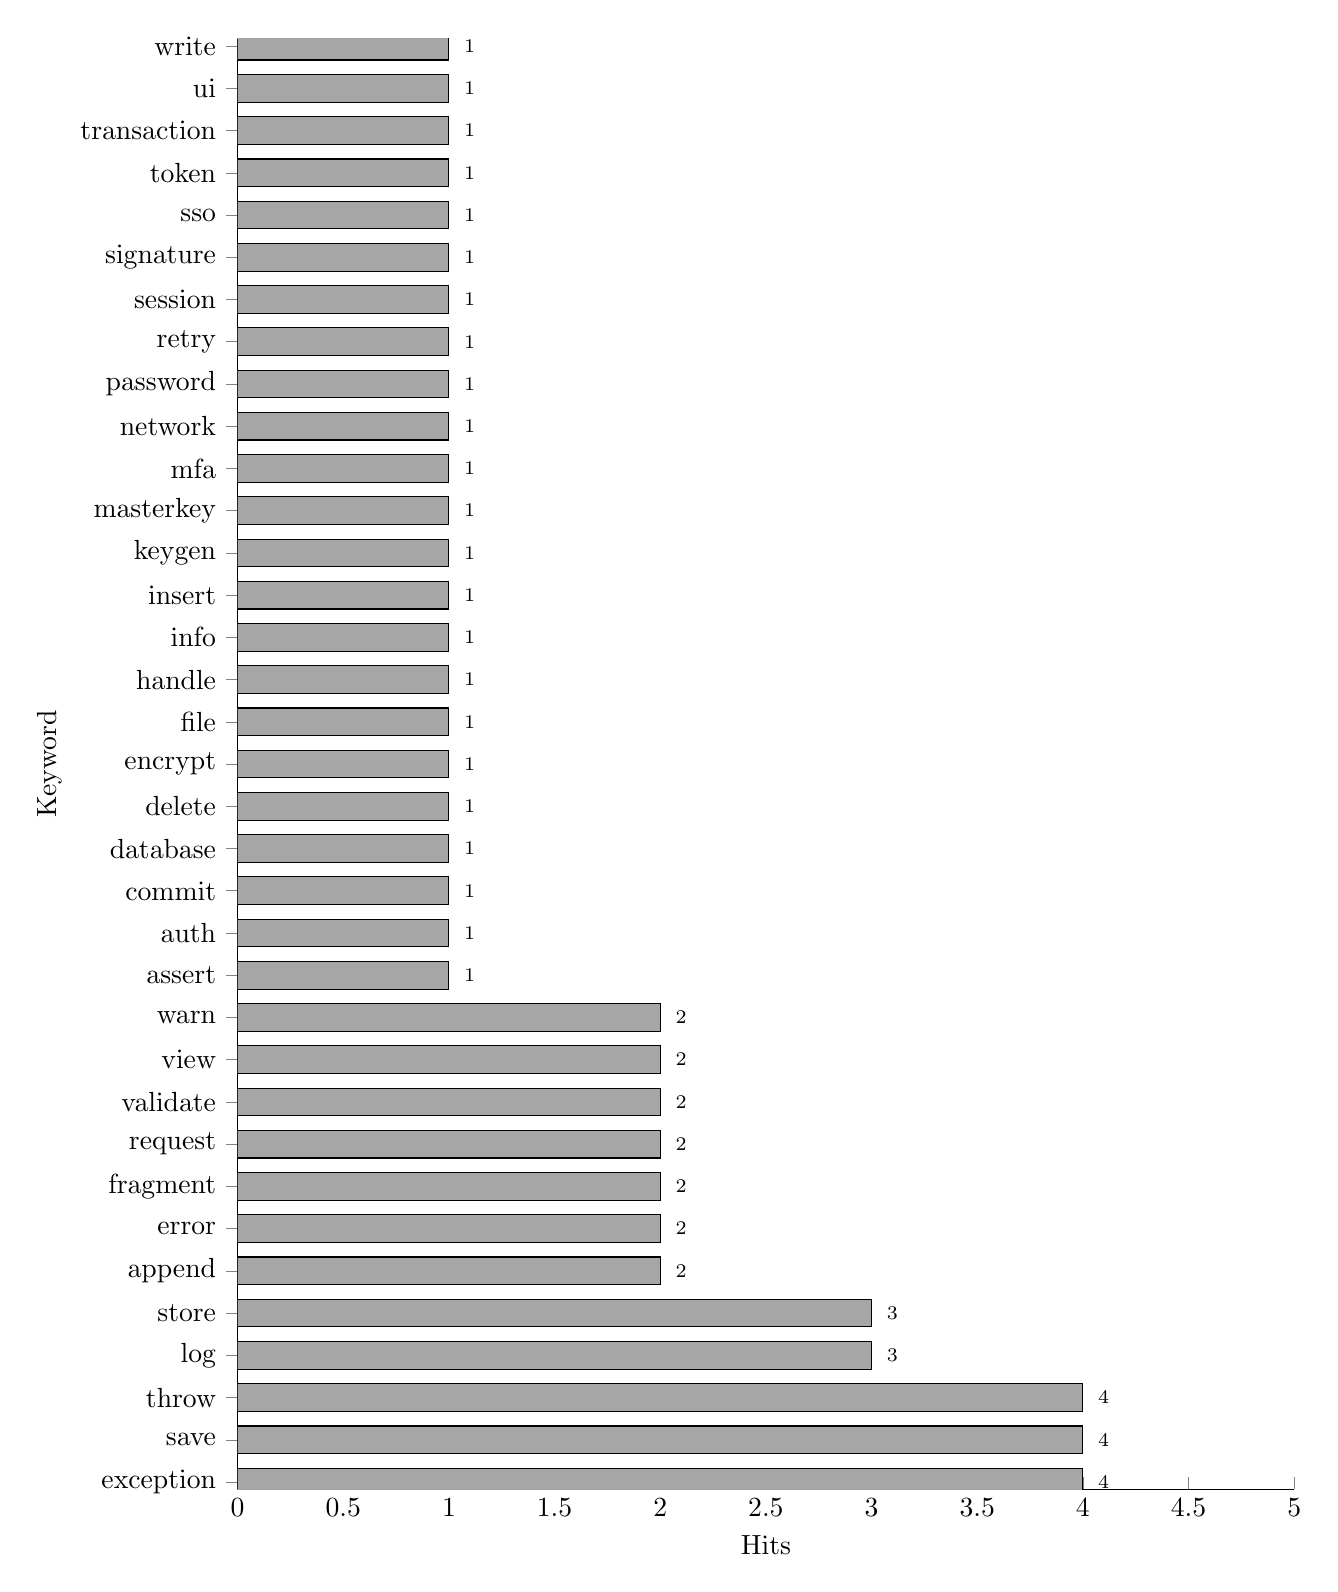
\begin{tikzpicture}
      \begin{axis}[
        width=15cm,
        height=20cm,
        xbar,
        bar width=10pt,
        symbolic y coords={
          exception,save,throw,log,store,append,error,fragment,request,validate,
          view,warn,assert,auth,commit,database,delete,encrypt,file,handle,info,
          insert,keygen,masterkey,mfa,network,password,retry,session,signature,
          sso,token,transaction,ui,write},
        ytick=data,
        tick label style={font=\normalsize},
        enlarge y limits=0.005,
        xlabel={Hits},
        ylabel={Keyword},
        xmin=0, xmax=5,
        nodes near coords,
        every node near coord/.append style={font=\scriptsize,xshift=2pt},
        axis x line*=bottom,
        axis y line*=left
      ]
        \addplot[xbar,fill=gray!70] coordinates {
          (4,exception) (4,save) (4,throw)
          (3,log) (3,store)
          (2,append) (2,error) (2,fragment) (2,request) (2,validate)
          (2,view) (2,warn)
          (1,assert) (1,auth) (1,commit) (1,database) (1,delete)
          (1,encrypt) (1,file) (1,handle) (1,info) (1,insert) (1,keygen)
          (1,masterkey) (1,mfa) (1,network) (1,password) (1,retry)
          (1,session) (1,signature) (1,sso) (1,token) (1,transaction)
          (1,ui) (1,write)
        };
      \end{axis}
    \end{tikzpicture}
    \caption{All keywords resulting in incorrect categorization for version diff A}
    \label{fig:keyword_incorrect_trigger_A_full_rotated}
\end{figure}
\end{comment}

\newpage
\begin{figure}
    \centering
    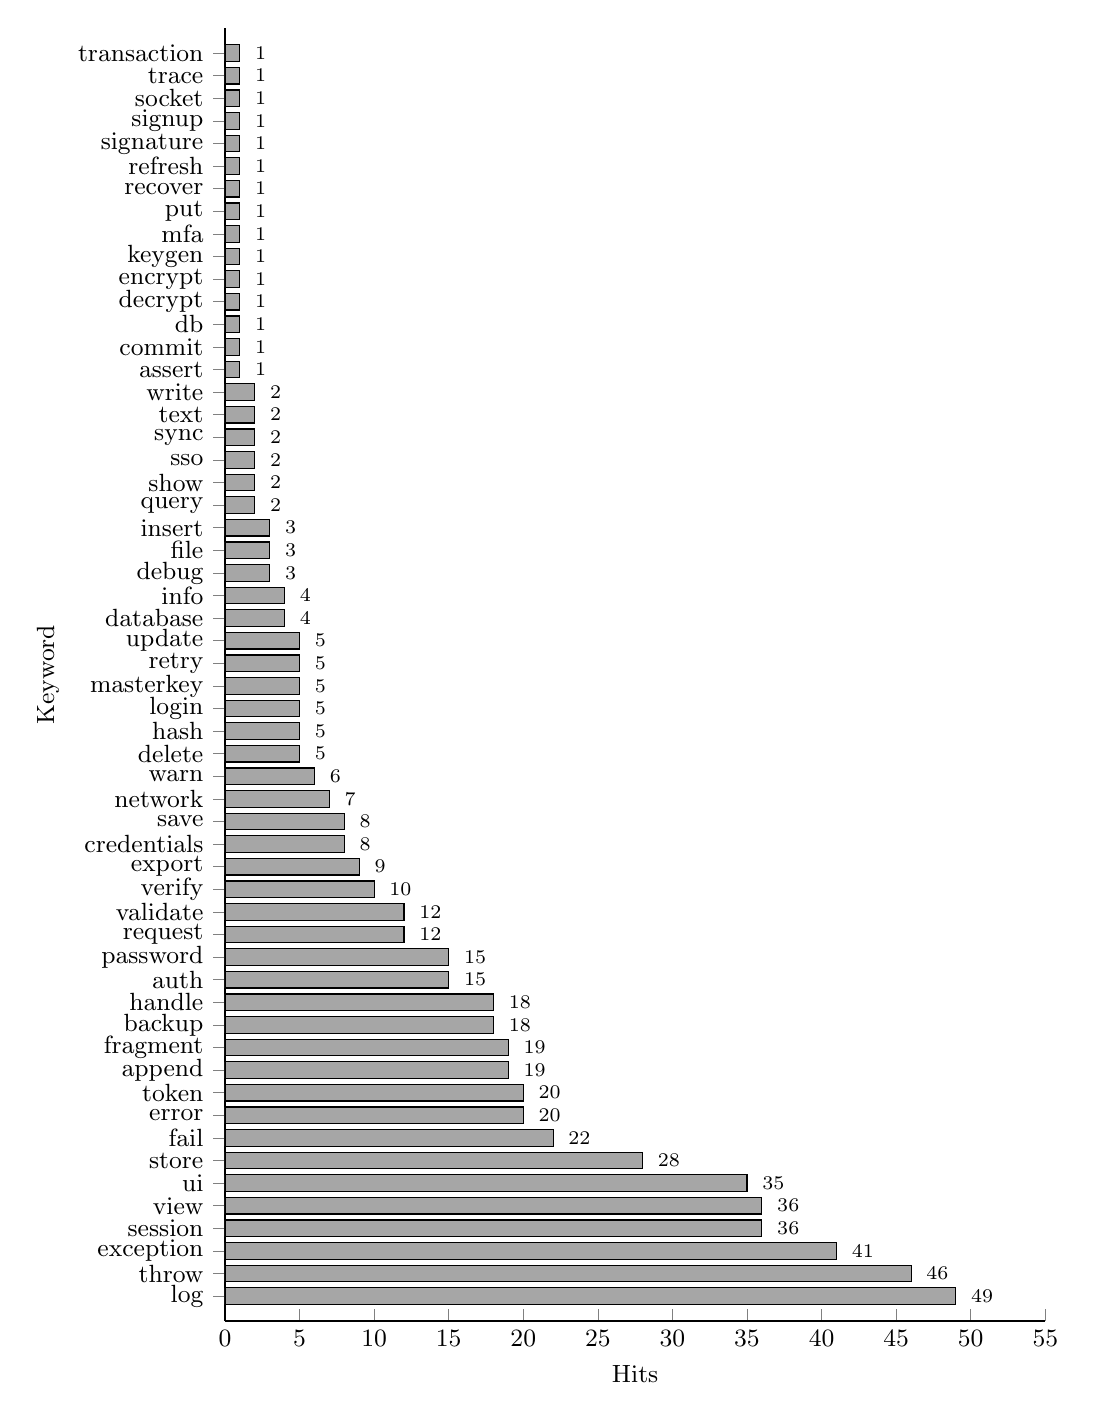
\begin{tikzpicture}
      \begin{axis}[
        width=12cm,
        height=18cm,
        xbar,
        bar width=6pt,
        font=\small,
        symbolic y coords={
            log,throw,exception,session,view,ui,store,fail,error,token,
            append,fragment,backup,handle,auth,password,request,validate,
            verify,export,credentials,save,network,warn,delete,hash,login,
            masterkey,retry,update,database,info,debug,file,insert,query,
            show,sso,sync,text,write,assert,commit,db,decrypt,encrypt,
            keygen,mfa,put,recover,refresh,signature,signup,socket,trace,
            transaction},
        ytick=data,
        tick label style={font=\small},
        enlarge y limits=0.02,
        xlabel={Hits},
        ylabel={Keyword},
        xmin=0, xmax=55,
        nodes near coords,
        every node near coord/.append style={font=\scriptsize,xshift=2pt},
        axis x line*=bottom,
        axis y line*=left
      ]
        \addplot[xbar,fill=gray!70] coordinates {
          (49,log) (46,throw) (41,exception) (36,session) (36,view)
          (35,ui) (28,store) (22,fail) (20,error) (20,token)
          (19,append) (19,fragment) (18,backup) (18,handle)
          (15,auth) (15,password) (12,request) (12,validate)
          (10,verify) (9,export) (8,credentials) (8,save)
          (7,network) (6,warn) (5,delete) (5,hash) (5,login)
          (5,masterkey) (5,retry) (5,update) (4,database)
          (4,info) (3,debug) (3,file) (3,insert) (2,query)
          (2,show) (2,sso) (2,sync) (2,text) (2,write)
          (1,assert) (1,commit) (1,db) (1,decrypt) (1,encrypt)
          (1,keygen) (1,mfa) (1,put) (1,recover) (1,refresh)
          (1,signature) (1,signup) (1,socket) (1,trace)
          (1,transaction)
        };
      \end{axis}
    \end{tikzpicture}
    \caption{All keyword hits generating categorizations in version diff A}
    \label{fig:commonly_used_words_A_full}
\end{figure}

\begin{figure}
    \centering
    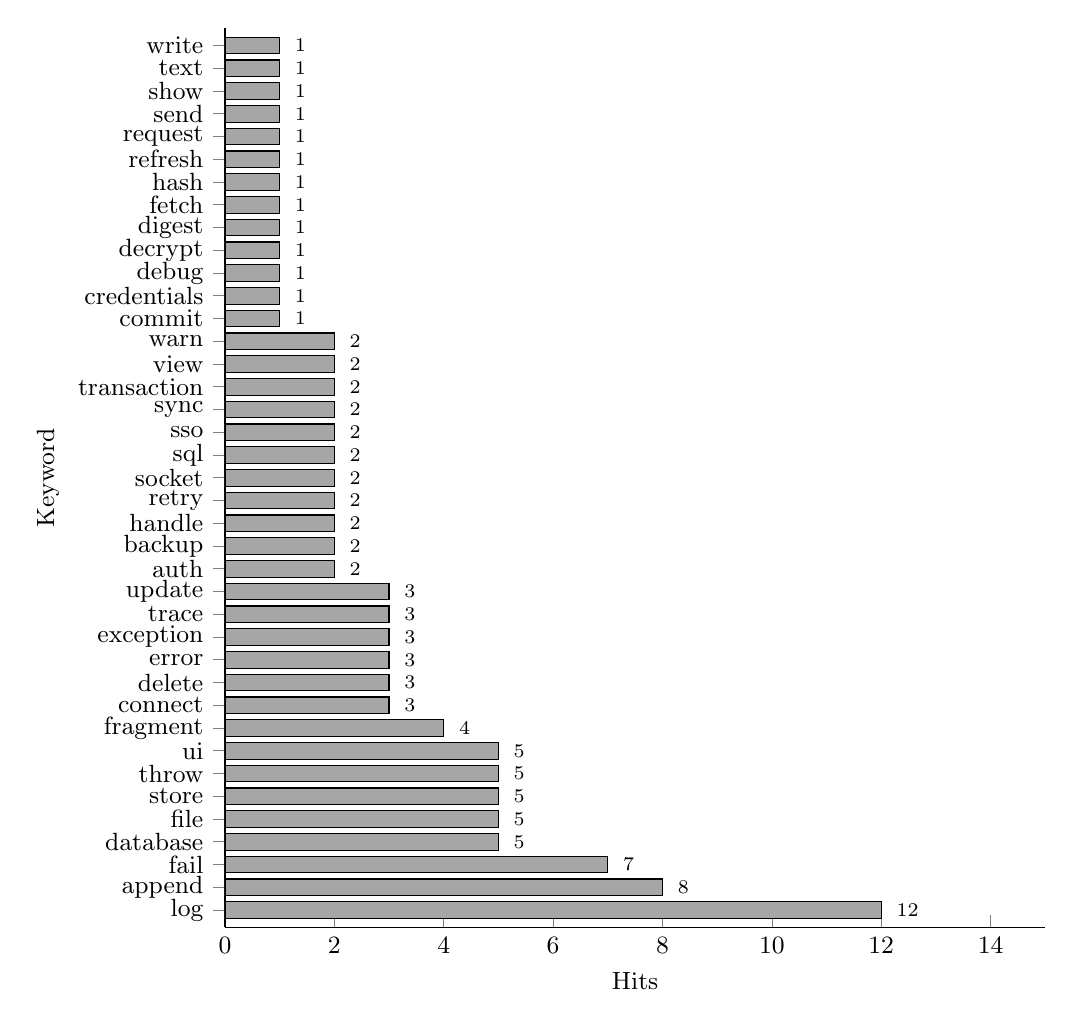
\begin{tikzpicture}
      \begin{axis}[
        width=12cm,
        height=13cm,
        xbar,
        bar width=6pt,
        font=\small,
        symbolic y coords={
            log,append,fail,database,file,store,throw,ui,fragment,connect,
            delete,error,exception,trace,update,auth,backup,handle,retry,
            socket,sql,sso,sync,transaction,view,warn,commit,credentials,
            debug,decrypt,digest,fetch,hash,refresh,request,send,show,text,
            write},
        ytick=data,
        tick label style={font=\small},
        enlarge y limits=0.02,
        xlabel={Hits},
        ylabel={Keyword},
        xmin=0, xmax=15,
        nodes near coords,
        every node near coord/.append style={font=\scriptsize,xshift=2pt},
        axis x line*=bottom,
        axis y line*=left
      ]
        \addplot[xbar,fill=gray!70] coordinates {
          (12,log) (8,append) (7,fail) (5,database) (5,file) (5,store)
          (5,throw) (5,ui) (4,fragment) (3,connect) (3,delete) (3,error)
          (3,exception) (3,trace) (3,update) (2,auth) (2,backup) (2,handle)
          (2,retry) (2,socket) (2,sql) (2,sso) (2,sync) (2,transaction)
          (2,view) (2,warn) (1,commit) (1,credentials) (1,debug) (1,decrypt)
          (1,digest) (1,fetch) (1,hash) (1,refresh) (1,request) (1,send)
          (1,show) (1,text) (1,write)
        };
      \end{axis}
    \end{tikzpicture}
    \caption{All keyword hits generating categorizations in version diff B}
    \label{fig:commonly_used_words_B_full}
\end{figure}

\begin{figure}
    \centering
    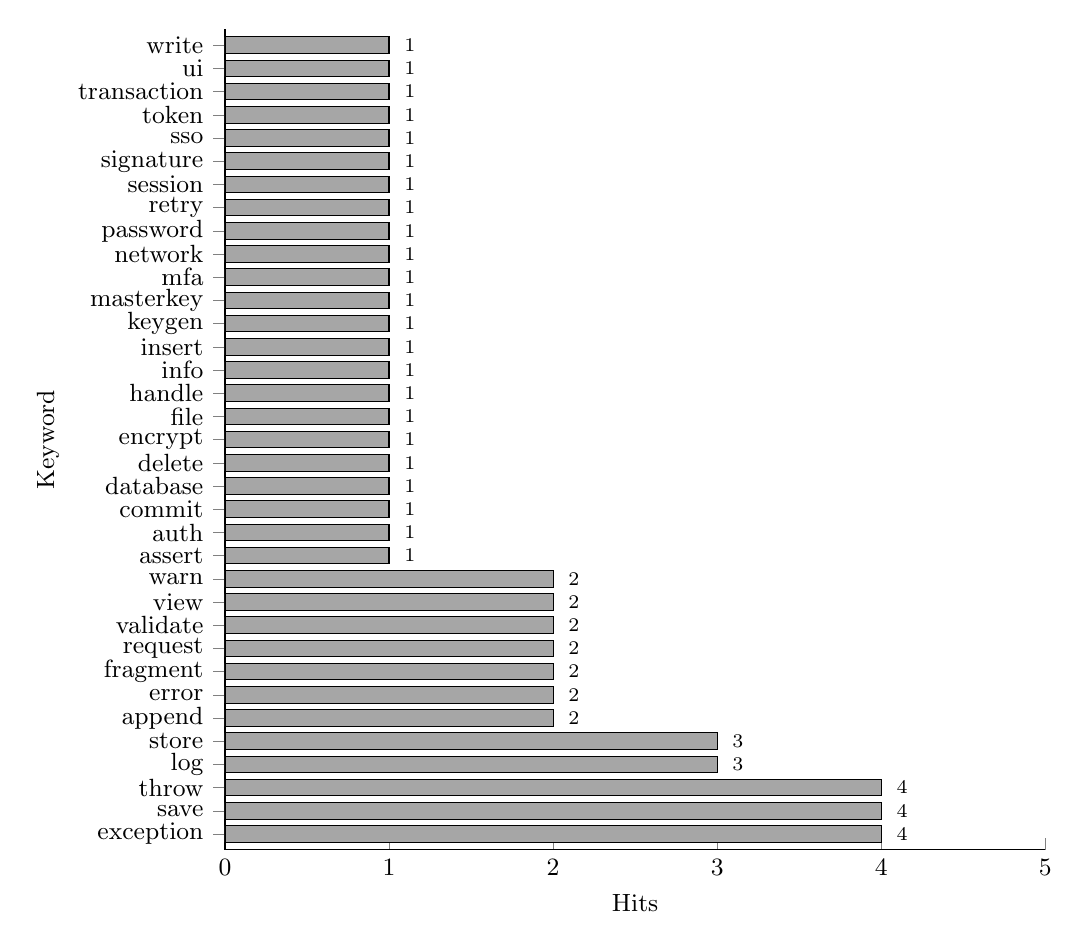
\begin{tikzpicture}
      \begin{axis}[
        width=12cm,
        height=12cm,
        xbar,
        bar width=6pt,
        font=\small,
        symbolic y coords={
          exception,save,throw,log,store,append,error,fragment,request,validate,
          view,warn,assert,auth,commit,database,delete,encrypt,file,handle,info,
          insert,keygen,masterkey,mfa,network,password,retry,session,signature,
          sso,token,transaction,ui,write},
        ytick=data,
        tick label style={font=\small},
        enlarge y limits=0.02,
        xlabel={Hits},
        ylabel={Keyword},
        xmin=0, xmax=5,
        xtick={0,1,2,3,4,5}, % <- force clean integer ticks
        nodes near coords,
        every node near coord/.append style={font=\scriptsize,xshift=2pt},
        axis x line*=bottom,
        axis y line*=left
      ]
        \addplot[xbar,fill=gray!70] coordinates {
          (4,exception) (4,save) (4,throw)
          (3,log) (3,store)
          (2,append) (2,error) (2,fragment) (2,request) (2,validate)
          (2,view) (2,warn)
          (1,assert) (1,auth) (1,commit) (1,database) (1,delete)
          (1,encrypt) (1,file) (1,handle) (1,info) (1,insert) (1,keygen)
          (1,masterkey) (1,mfa) (1,network) (1,password) (1,retry)
          (1,session) (1,signature) (1,sso) (1,token) (1,transaction)
          (1,ui) (1,write)
        };
      \end{axis}
    \end{tikzpicture}
    \caption{All keywords resulting in incorrect categorization for version diff A}
    \label{fig:keyword_incorrect_trigger_A_full}
\end{figure}



\end{appendices}


\end{document}
